\documentclass[10pt]{article}
\usepackage[
    letterpaper,
    top=19mm,
    bottom=25.4mm,
    left=17.3mm,
    right=17.3mm,
    includefoot,
    footskip=14mm
]{geometry}


\usepackage{amsmath}
\usepackage[utf8]{inputenx}
\usepackage[spanish]{babel}
\usepackage[pdftex]{graphicx} 	%  uso de graficos en general		%  poder poner dos graficos como parte de uno
\usepackage{fancyhdr} 		%  encabezado diferente para pag pares e impares
\usepackage{epstopdf} 		%  Convertir .eps a .pdf (si fuera necesario)
\usepackage{titling}
\usepackage{fancyvrb,fancybox,calc} 
\usepackage[svgnames]{xcolor} 
\usepackage{enumerate}
\usepackage{adjustbox}
\usepackage{tabu}
\usepackage{multicol}
\usepackage{float}
\usepackage{subcaption}
\usepackage{setspace}
\usepackage{tabularx}
\usepackage{booktabs}
\usepackage{amsmath}
\usepackage{hyperref}
\usepackage{url}
\usepackage{longtable}


\newcommand{\HRule}{\rule{\linewidth}{0.5mm}}

% Secciones preliminares (antes de "Introducción"): sin número, pero
% igualmente listadas en el índice.
\newcommand{\prefsection}[1]{%
  \phantomsection
  \section*{#1}%
  \addcontentsline{toc}{section}{#1}%
}
% \prefsectionnotitle agrega la entrada de nivel "section" solo al índice,
% sin imprimir ningún título en la página (usado para "Prefacio").
\newcommand{\prefsectionnotitle}[1]{%
  \phantomsection
  \addcontentsline{toc}{section}{#1}%
}
\newcommand{\prefsubsection}[1]{%
  \phantomsection
  \subsection*{#1}%
  \addcontentsline{toc}{subsection}{#1}%
}
%\usepackage[usenames,dvipsnames]{color}
\DeclareGraphicsExtensions{.pdf,.png,.jpg} % busca en este orden! 

% Texto de párrafo en 12pt (los títulos usan \Large/\huge/etc. y no cambian)
\renewcommand{\normalsize}{\fontsize{12}{14.5}\selectfont}
\normalsize

\setlength{\parskip}{6pt}
\parindent=2em          % sangría de primera línea
\setlength{\parskip}{6pt} % espacio después de cada párrafo
\onehalfspacing  % interlineado 1.5

\definecolor{light-gray}{gray}{0.94}
\definecolor{textgray}{gray}{0.5}
\newenvironment{verbcode}{\VerbatimEnvironment
    \begin{Sbox} \color{textgray}\scriptsize
    \begin{minipage}{\linewidth+2\fboxsep-2\fboxrule-12pt}    
    \begin{Verbatim}
}{\end{Verbatim}  
    \end{minipage}   
    \end{Sbox} \color{black}\normalsize
    \fcolorbox{black}{light-gray}{\TheSbox} 
} 


\begin{document}
\renewcommand{\tablename}{Tabla}
\begin{center}

% Title
{ \huge \bfseries  SYNAP \\[0.5cm] }
{ \Large \emph  { Desarrollo de un sistema de gestión de equipamiento médico basado \\[0.1cm]
en el Hospital Alemán} \\[0.2cm] }

\vspace{1cm}


\includegraphics[width=10cm]{fotos/logo_itba.png}

\vspace{1cm}

\emph {\Large Proyecto final de Carrera para la obtención del título de Bioingeniero}\\[0.2cm]
\vspace{0.5cm}

% Integrantes
\textsc{Autoras:}\  Inés María  Steverlynck (63667), \ Camila Barbagelata (63047)\\[0.2cm]

\vspace{0.5cm}

% Author and supervisor
\textsc{Tutora:}\  Siomara Figueredo\\[0.2cm]

\textsc{Co-tutor:}\  Carlos Lazzarino\\[0.5cm]

\large \textsc{Octubre 2026}\\[0.1cm]

\vspace{0.5cm}


\end{center}

\vspace{0.2cm}


\pagestyle{fancy}
\headheight=60pt 	%para cambiar el tamaño del encabezado
\fancyhead[L]	{	Proyecto final de carrera - 94.16 	}
\fancyhead[R] 	{	ITBA  }
\fancyfoot[C]	{	\thepage  }
\thispagestyle{empty}

\pagenumbering{roman}

%=======================================================================================================
\newpage
\prefsectionnotitle{Prefacio}

\prefsubsection{Agradecimientos}
A nuestra tutora, Siomara Figueredo, jefa del servicio de Bioingeniería del Hospital Alemán, por su guía constante, por el tiempo que nos dedicó y por la confianza que depositó en nosotras. Su conocimiento del servicio fue fundamental para que SYNAP respondiera a la forma real de trabajar de Bioingeniería.

Al Hospital Alemán, por abrirnos las puertas de su servicio de Bioingeniería y facilitarnos la información necesaria para desarrollar este proyecto.

A los coordinadores, bioingenieros y técnicos del servicio, que nos explicaron cómo trabajan, respondieron la encuesta y, al conocer el sistema, compartieron su opinión con generosidad. Sus aportes dieron forma a gran parte de lo que hoy hace SYNAP.

A nuestro co-tutor, Carlos Lazzarino, por su acompañamiento y sus aportes durante el desarrollo del trabajo.

A la cátedra de Proyecto Final de Carrera, por acompañarnos a lo largo de todo el proyecto.

Al Instituto Tecnológico de Buenos Aires, nuestra casa de estudios durante toda la carrera, por la formación que nos dio y que nos permite comenzar esta nueva etapa como profesionales.

A nuestras familias, por acompañarnos sin condiciones durante la carrera y este proyecto, y por recordarnos siempre lo orgullosos que están de nosotras.

A nuestros amigos, que caminaron a nuestro lado en este recorrido y celebran con nosotras este logro.

%=======================================================================================================
\newpage
\prefsubsection{Resumen}

El equipamiento médico condiciona de manera directa las prestaciones que un hospital puede ofrecer, y su disponibilidad depende de cómo se gestiona su mantenimiento. En el Hospital Alemán, el servicio de Bioingeniería utiliza IBM Maximo, un sistema de propósito general que no está pensado para un servicio hospitalario. Por eso, tareas como la planificación de preventivos, el aviso de fallas y el seguimiento del stock se resuelven por fuera, en planillas, llamados y papel. 

Este trabajo expone el diseño y desarrollo de SYNAP, un prototipo de sistema web que centraliza la información de cada equipo. Al escanear el código QR de su etiqueta se accede a su ficha, se reportan fallas y se siguen sus órdenes de trabajo, y la plataforma suma además la gestión de stock y un panel de indicadores. Los requerimientos surgieron de una encuesta al servicio, del análisis de las exportaciones de Maximo y del marco normativo y teórico. 

El sistema se desarrolló de forma iterativa con FastAPI, PostgreSQL y React, con un diseño responsive para computadoras y celulares. Como resultado, se obtuvo un sistema con cuatro perfiles de usuario que calcula el riesgo de cada equipo, sugiere la prioridad de las órdenes y mide el cumplimiento de preventivos, la inactividad y los tiempos medios entre fallas y de reparación. Para validarlo en un caso de uso real, se migraron los 6.178 activos del inventario del hospital, de modo que la plataforma opera con los datos reales del servicio y no solo con datos de prueba. SYNAP muestra así que es posible una gestión del equipamiento médico más trazable, ágil y basada en datos.


\vspace{\baselineskip}
\noindent\textbf{Palabras clave}: gestión de equipamiento médico, bioingeniería, ingeniería clínica, mantenimiento preventivo, trazabilidad, gestión de tecnologías sanitarias, sistema de gestión de mantenimiento (CMMS).


%=======================================================================================================
\newpage
{\centering\normalfont\scshape\LARGE Tabla de contenidos\par}
\addcontentsline{toc}{section}{Tabla de contenidos}

\renewcommand{\contentsname}{}
\vspace{-\baselineskip}
\tableofcontents

%=======================================================================================================
\newpage
\prefsubsection{Lista de Figuras}
\renewcommand{\listfigurename}{}
\vspace{-\baselineskip}
\listoffigures

%=======================================================================================================
\newpage
\prefsubsection{Lista de Tablas}
\renewcommand{\listtablename}{}
\vspace{-\baselineskip}
\listoftables

%=======================================================================================================
\newpage
\prefsubsection{Índice de abreviaturas}
\begingroup
\renewcommand{\arraystretch}{1.05}
\begin{tabular}{@{}p{0.17\linewidth}@{\hspace{0.02\linewidth}}p{0.79\linewidth}@{}}
\textbf{ANMAT} & Administración Nacional de Medicamentos, Alimentos y Tecnología Médica \\
\textbf{API} & \textit{Application Programming Interface} (interfaz de programación de aplicaciones) \\
\textbf{CMMS} & \textit{Computerized Maintenance Management System} (Sistema Computarizado para la Gestión del Mantenimiento) \\
\textbf{CSV} & \textit{Comma-Separated Values} (valores separados por comas), formato de archivo para tablas \\
\textbf{CU} & Caso de uso \\
\textbf{DNI} & Documento Nacional de Identidad \\
\textbf{FMS} & \textit{Facilities Management Services}, área hospitalaria de infraestructura y servicios técnicos \\
\textbf{HTTP} & \textit{Hypertext Transfer Protocol} (Protocolo de Transferencia de Hipertexto) \\
\textbf{HTTPS} & \textit{Hypertext Transfer Protocol Secure} (versión segura del protocolo HTTP) \\
\textbf{IEC} & \textit{International Electrotechnical Commission} (Comisión Electrotécnica Internacional) \\
\textbf{IRAM} & Instituto Argentino de Normalización y Certificación \\
\textbf{JSON} & \textit{JavaScript Object Notation}, formato de texto para intercambiar datos \\
\textbf{JWT} & \textit{JSON Web Token} (token web JSON) \\
\textbf{MP} & Mantenimiento preventivo \\
\textbf{MTBF} & \textit{Mean Time Between Failures} (tiempo medio entre fallas) \\
\textbf{MTTR} & \textit{Mean Time To Repair} (tiempo medio de reparación) \\
\textbf{OMS} & Organización Mundial de la Salud \\
\textbf{OT} & Orden de trabajo \\
\textbf{PDF} & \textit{Portable Document Format} (formato de documento portátil) \\
\textbf{PMA} & Producto médico activo \\
\textbf{PNGCAM} & Programa Nacional de Garantía de Calidad de la Atención Médica \\
\textbf{PRIUX} & Tablas de riesgo propias del Hospital Alemán \\
\textbf{QR} & \textit{Quick Response} (respuesta rápida), código bidimensional \\
\textbf{RF} & Requerimiento funcional \\
\textbf{RNF} & Requerimiento no funcional \\
\textbf{SMTP} & \textit{Simple Mail Transfer Protocol} (protocolo simple de transferencia de correo) \\
\textbf{SQL} & \textit{Structured Query Language} (lenguaje de consulta estructurado) \\
\end{tabular}
\endgroup


%=======================================================================================================
\newpage
\pagenumbering{arabic}
\setcounter{page}{1}
\fancyfoot[C]	{	Página \thepage\ de \pageref{LastPage}  }

\section{Introducción}
\subsection{Contexto y planteamiento del problema}
\label{sec:contexto-problema}

El equipamiento médico de un centro de salud forma parte de la infraestructura sobre la que se apoya la atención clínica. Un respirador, un monitor multiparamétrico o un ecógrafo no son solo bienes administrativos dentro del patrimonio de una institución, sino recursos cuya disponibilidad condiciona de manera directa qué prestaciones puede ofrecer un hospital y en qué tiempos. Cuando un equipo queda fuera de servicio o no se encuentra en las condiciones adecuadas, el efecto se traslada al paciente en forma de estudios postergados, prácticas inseguras, diagnósticos erróneos o procedimientos reprogramados, obstaculizando el flujo de atención del centro y comprometiendo el sistema de salud. Esa disponibilidad y estado del equipo se define a lo largo de toda su vida útil, y depende en gran parte de cómo se administra su mantenimiento y de cómo y dónde se registra la información sobre el mismo \cite{ministerio2002}.

Por esa razón, las instituciones de salud cuentan con servicios de Bioingeniería o Ingeniería Clínica, que son responsables de sostener el parque tecnológico mediante una gestión efectiva: planificación de los mantenimientos preventivos, respuesta ante fallas, control del inventario y trazabilidad de cada activo \cite{cardoso_waqued}. Una gran parte de esta tarea es trabajo sobre información que debería estar disponible; un servicio necesita saber qué equipos tiene, a qué área pertenecen, en qué estado se encuentran, cuándo se intervino cada uno, a cargo de quien estuvo y qué ocurrió en esa intervención. Cuando esos datos se encuentran incompletos, dispersos entre planillas o resultan difíciles de recuperar, la gestión termina apoyándose en la memoria y la experiencia de quienes integran el área, limitando la eficiencia de la misma.

Como se menciona en la tesis doctoral de Bertelli \cite{bertelli2023} sobre la gestión del equipamiento médico del Ministerio de Salud de la Ciudad Autónoma de Buenos Aires, este equipamiento requiere que se lo gestione y se invierta tiempo, recursos humanos y materiales para su incorporación, buen uso, mantenimiento y hasta su desafectación. 

Para ordenar este trabajo en las instituciones existen los sistemas de gestión de mantenimiento, conocidos como CMMS por sus siglas en inglés (Computerized Maintenance Management System). Estos sistemas centralizan el inventario de equipos, la programación de las intervenciones y el registro de lo realizado sobre cada uno. Lo que suele ocurrir en el ámbito hospitalario es que se adopta un sistema que nunca fue concebido para un hospital, ya que lo incorpora el área de mantenimiento edilicio para administrar ascensores, calderas e instalaciones, y una vez implementado se lo extiende al equipamiento médico. De esta forma, aparecen desajustes por el simple hecho de ser un sistema que no tiene en cuenta que los equipos médicos se trasladan entre sectores, que las fallas deben ser reportadas por personal asistencial en medio de un turno, o que cualquier intervención tiene que organizarse de acuerdo a la disponibilidad clínica. Una de las coordinadoras del servicio de Bioingeniería del Hospital Alemán lo expresó en la encuesta realizada para este trabajo, al señalar que el sistema que utilizan tiene muchos campos que no les sirven por tratarse de un programa genérico pensado para la industria (sección~\ref{sec:encuesta}).

\subsection{Propuesta y justificación}
\label{sec:propuesta-justificacion}
Frente a ese escenario, el presente documento detalla el diseño y desarrollo de SYNAP, un sistema web de gestión de equipamiento médico pensado específicamente para un servicio hospitalario de Bioingeniería, que reúne en una única plataforma la información de cada activo, las órdenes de trabajo preventivas y correctivas, el stock de insumos y repuestos y los indicadores de desempeño del área, entre otras funciones. El nombre remite a la sinapsis neuronal, ya que lo que el sistema busca aportar son justamente las conexiones que hoy faltan o funcionan de manera débil entre el equipo registrado, la falla que se le reporta, la orden de trabajo que esa falla genera y el repuesto que se consume para resolverla.

El proyecto aquí presentado está basado en el Hospital Alemán, institución privada de la Ciudad Autónoma de Buenos Aires, que actualmente gestiona su equipamiento médico con IBM Maximo \cite{ibm_maximo}. Tanto el desarrollo como la validación de SYNAP se llevan adelante junto al equipo de Bioingeniería de la institución, que es fuente de los requerimientos que definen la estructura del sistema y, además, su destinatario. Esto permitió incorporar observaciones y necesidades reales a lo largo del proceso y no una vez que el sistema ya estaba cerrado, con el propósito de que el equipo pueda adoptarlo de forma natural en su trabajo cotidiano.

Se trata de un prototipo, desarrollado con una base de prueba y validado luego con la información real del hospital (sección~\ref{sec:integracion-datos}). Su puesta en funcionamiento como reemplazo del sistema actual implicaría, además, un despliegue en la infraestructura del hospital, la capacitación del personal y una revisión de los recaudos de seguridad sobre la información confidencial de la institución, tareas que exceden el alcance de este trabajo.

Los objetivos que guiaron el desarrollo se presentan a continuación, separados entre aquellos que el sistema debe cumplir necesariamente y aquellos que amplían su alcance en caso de que el avance del trabajo lo permita.

\subsection{Objetivos}
\label{sec:objetivos}
\subsubsection{Objetivo general}
Desarrollar un prototipo funcional de sistema web para la gestión de equipos médicos en el Hospital
Alemán, que centralice su información y funcione como herramienta de soporte para el servicio de
Bioingeniería.

\subsubsection{Objetivos de mínima}
\label{sec:objetivos-minima}
\begin{itemize}
    \item Desarrollar una interfaz web responsive para la gestión del equipamiento médico, que
permita consultar la información de cada activo y registrar y clasificar las fallas
reportadas.
    \item Proveer un entorno para la apertura, seguimiento y cierre de órdenes de trabajo del área de
Bioingeniería, y la consulta de los mantenimientos preventivos programados.
    \item Incorporar al sistema un módulo de gestión de stock de insumos y repuestos
vinculado a las órdenes de trabajo del servicio de Bioingeniería.
    \item Implementar un panel de gestión (\emph {dashboard}) para perfiles de jefatura que permita la
visualización de indicadores clave de desempeño (\emph {KPIs}).
    \item Migrar e integrar la información existente en las bases de datos del Hospital Alemán
al sistema, validando su funcionamiento en un caso de uso real.
\end{itemize}

\subsubsection{Objetivos de máxima}
\begin{itemize}
    \item Permitir el contacto directo del bioingeniero responsable del equipo, facilitando la
comunicación entre usuarios y el servicio de Bioingeniería.
    \item Integrar un sistema de notificaciones que centralice las órdenes de trabajo correctivas
en bandejas de entrada específicas.
    \item Analizar el historial de órdenes de trabajo para identificar patrones de fallas y tiempos
de resolución, generando información de soporte para la toma de decisiones sobre el
parque tecnológico.
\end{itemize}

\subsection{Estructura del documento}
El informe continúa con el estado del arte y el marco teórico, que reúnen los antecedentes en sistemas de gestión de equipamiento médico y los conceptos que fundamentan las decisiones de diseño. El capítulo~\ref{sec:diseno-desarrollo} describe el diseño y desarrollo del sistema, desde el relevamiento realizado en el servicio de Bioingeniería y los requerimientos que surgieron de él hasta el modelo de datos, la arquitectura y las tecnologías, el desarrollo de cada módulo y la integración de los datos del hospital. Los resultados se presentan en el capítulo~\ref{sec:resultados}, que incluye la validación con el servicio, y el capítulo~\ref{sec:discusion} los discute frente a los antecedentes y analiza sus limitaciones. El capítulo~\ref{sec:futuro} plantea las perspectivas futuras y el capítulo~\ref{sec:conclusiones} reúne las conclusiones del trabajo. Los anexos reúnen la encuesta, los casos de uso detallados, los requerimientos del sistema y los manuales de uso.

%=======================================================================================================
\newpage
\section{Estado del arte}
\label{sec:estado-arte}
Diversos trabajos académicos abordaron la gestión del equipamiento médico mediante el desarrollo de sistemas informáticos propios, desde plataformas de soporte a los procesos de gestión basadas en los lineamientos de la OMS \cite{miranda_takayama2017} hasta sistemas para organizar el mantenimiento preventivo y correctivo \cite{khider_hamza2023} o modelos para priorizar las solicitudes de mantenimiento \cite{hamdi2012}. Sin embargo, se trata de desarrollos pensados para contextos institucionales y normativos ajenos al argentino, por lo que este apartado se centra en las soluciones que efectivamente se utilizan en el país. El Hospital Alemán trabaja actualmente con IBM Maximo \cite{ibm_maximo}, una plataforma de gestión de activos concebida para la industria en general que los hospitales adaptan a la gestión de su equipamiento médico; lo que limita su ajuste a las necesidades del servicio (véase la sección~\ref{sec:encuesta}).

A diferencia de Maximo, existen herramientas concebidas desde su origen para la ingeniería clínica, y cada una de ellas pone el énfasis en un aspecto distinto de la gestión. Neovero, un sistema de origen brasileño, se orienta a la gestión integral del parque, acompañando a cada equipo a lo largo de todo su ciclo de vida, desde la planificación de la compra hasta la obsolescencia \cite{neovero}. Su aporte más relevante es la clasificación de los equipos según su criticidad, que define la prioridad con la que se atiende cada falla y los tiempos de respuesta esperados, de modo que un respirador detenido no espera lo mismo que un equipo de menor riesgo. Según la propia empresa, el sistema ha sido implementado en instituciones argentinas como Fleni, la Fundación Favaloro y el Hospital de Alta Complejidad El Cruce \cite{neovero}.

Por otro lado, se tiene Kibbo de la empresa Leex, que ataca otro punto crítico: el momento en que se detecta la falla. En lugar de depender de un llamado o de un pedido informal, el personal de salud escanea el código QR del equipo desde su celular y el reporte llega directamente al área de bioingeniería, identificando sin ambigüedad de qué equipo se trata. El mismo código le da acceso, además, a los manuales del equipo \cite{leex_medical}. Equipasis es otro sistema que fue presentado en las Jornadas Argentinas de Informática, y que principalmente pone el foco en la toma de decisiones. Está diseñado para registrar los datos de cada equipo de manera parametrizada para poder filtrarlos y construir indicadores, lo que permitió a sus usuarios medir la eficiencia de cada servicio y de cada proveedor, y admite la gestión de varios centros desde una misma plataforma \cite{equipasis}.

Estos antecedentes muestran que las funciones centrales de un sistema de gestión de equipamiento médico ya están resueltas por distintas herramientas. En el Hospital Alemán, lo que falla no son tanto las funciones como la manera en que se conectan entre ellas, y ahí se ubica SYNAP. No busca reemplazar a Maximo ni sumar otro producto a la lista, sino reforzar esas conexiones a partir de los datos y criterios que el servicio ya maneja.

%=======================================================================================================
\newpage
\section{Marco teórico}
\subsection{CMMS}
Un Sistema Computarizado para la Gestión del Mantenimiento (CMMS, por sus siglas en inglés) es una herramienta informática pensada para registrar, ordenar y analizar la información vinculada al inventario de equipos médicos y a su mantenimiento durante todo su ciclo de vida. Su principal aporte es reunir en una sola plataforma datos que de otro modo quedarían dispersos, y es justamente esa idea la que guía el diseño de SYNAP, cuya base de datos se organiza en torno al código de activo como identificador único de cada equipo.

A través de un CMMS es posible planificar y distribuir las tareas de mantenimiento y, al mismo tiempo, dejar constancia de cada intervención o evento que involucra a un equipo, de manera que su historia quede siempre disponible y sea trazable. Estos sistemas también permiten asignar prioridades según la urgencia de cada caso, algo que en SYNAP se resuelve mediante la clasificación de fallas por severidad, y canalizan los pedidos de insumos o reparaciones por una vía formal que reduce olvidos y malentendidos, razón por la cual el stock se vincula directamente con las órdenes de trabajo.

Quizás la ventaja más valiosa de estos sistemas sea la posibilidad de generar y analizar indicadores de desempeño, entre ellos la frecuencia de fallas, el tiempo medio entre fallas (MTBF) y el tiempo medio de reparación (MTTR). Con esa información se vuelve posible reconocer qué equipos son críticos, anticipar tendencias de falla y distribuir mejor los recursos técnicos y económicos, y por eso estos indicadores, junto con el cumplimiento del mantenimiento preventivo y el tiempo de inactividad, son los que conforman el dashboard de SYNAP orientado a jefatura.

\subsection{Marco normativo}
\label{sec:marco-normativo}
En Argentina, la gestión del equipamiento médico en uso se encuadra en la Ley 26.906, sancionada y publicada en el año 2013, que establece el régimen de trazabilidad y verificación de aptitud técnica de los productos médicos activos de salud en uso \cite{ley_26906}. Su sanción responde a una necesidad concreta, que es garantizar que un equipo destinado a la atención de pacientes conserve a lo largo de toda su vida útil las condiciones de seguridad y funcionamiento para las que fue fabricado, y no únicamente en el momento de su adquisición. La ley alcanza a la totalidad de los productos médicos activos de los establecimientos de salud públicos y privados del territorio nacional, y designa como autoridad de aplicación al Ministerio de Salud de la Nación.

El objeto de esa regulación se delimita con precisión en el artículo 3, que define como producto médico activo (PMA) a cualquier producto médico cuyo funcionamiento dependa de energía eléctrica o de una fuente de potencia distinta de la generada por el cuerpo humano o la gravedad, y que opere por conversión de esa energía. La misma definición excluye de manera expresa a aquellos productos destinados únicamente a transmitir energía, sustancias u otros elementos desde un PMA hacia el paciente sin provocar alteración significativa alguna. El criterio, que la ley toma del corpus normativo de la Administración Nacional de Medicamentos, Alimentos y Tecnología Médica (ANMAT) \cite{anmat_4306_1999}, traza una línea con consecuencias prácticas inmediatas sobre el alcance de cualquier inventario, ya que un respirador, un monitor multiparamétrico o una bomba de infusión quedan comprendidos, mientras que el circuito respiratorio o el latiguillo que los conecta al paciente no constituyen en sí mismos PMA aunque resulten imprescindibles para su funcionamiento.

Profundizando sobre la ley, el artículo 1 define tres objetos que conviene explicar por separado, dado que cada uno se traduce en requerimientos distintos para un sistema de gestión. El primero es la trazabilidad de los PMA, entendida en el artículo 3 como el conjunto de acciones y procedimientos técnicos que permiten identificar y registrar cada equipo en uso. El segundo es la trazabilidad metrológica, definida como la propiedad por la cual el resultado de una medición puede vincularse con referencias determinadas mediante una cadena ininterrumpida y documentada de calibraciones. El tercero es la creación o el fortalecimiento de los Servicios de Tecnología Biomédica, a los que la misma norma caracteriza como los encargados de gestionar en forma integral el parque tecnológico \cite{ley_26906}; en el contexto de SYNAP, el servicio de Bioingeniería del Hospital Alemán.

En este contexto, SYNAP se centra en la trazabilidad de los PMA. En la práctica, esto implica que cada equipo tenga un identificador único y que todas las intervenciones que recibe, desde las órdenes de trabajo y los mantenimientos preventivos hasta las fallas reportadas y los repuestos consumidos, queden vinculadas a él, de modo que su historia completa pueda recuperarse a partir de un único registro. Al mismo tiempo, SYNAP le da al servicio de Bioingeniería del Hospital Alemán una herramienta para cumplir una de las funciones que la ley le asigna, la de mantener documentada la verificación técnica y el mantenimiento de todos los equipos (art. 15, inc. g), y en ese sentido contribuye también al tercer componente de la ley, el fortalecimiento de los Servicios de Tecnología Biomédica.

La Ley 26.906 permaneció sin reglamentar durante casi una década, de modo que sus obligaciones estaban vigentes pero sin procedimientos concretos para cumplirlas, hasta que el Decreto 517/2023 aprobó su reglamentación \cite{decreto_517_2023}. 

Este decreto resulta relevante para el presente proyecto por dos razones. La primera es que establece una aplicación gradual de la ley, en la que el Ministerio de Salud irá definiendo qué tipos de equipos se incorporan primero al régimen y cómo se habilitan progresivamente los Servicios de Ingeniería Clínica, el área a la que está destinado este trabajo. La segunda es que precisa la obligación, ya prevista en la ley, de que cada establecimiento lleve un registro de los PMA en uso que permita su identificación y trazabilidad, se cargue en el Registro Federal de Establecimientos de Salud (REFES) y se actualice anualmente, lo que constituye el fundamento normativo directo del inventario centralizado que desarrolla este trabajo. Posteriormente, el Decreto 70/2023 derogó los artículos de la ley referidos a la habilitación de los PMA \cite{decreto_70_2023} y el Decreto 226/2024 adecuó la reglamentación a ese cambio \cite{decreto_226_2024}, aunque ambos mantuvieron vigentes las disposiciones sobre las que se apoya este trabajo.

En la misma semana en la que se publicó el decreto 517/2023, el Ministerio de Salud aprobó mediante la Resolución 2725/2023 las “Directrices de organización y funcionamiento de los Servicios de Ingeniería Clínica”, junto con un documento de procesos del plan de mantenimiento (véase la sección~\ref{sec:plan-mantenimiento}) y una grilla para la habilitación de estos servicios en los establecimientos de salud, todos incorporados al Programa Nacional de Garantía de Calidad de la Atención Médica (PNGCAM) \cite{res_2725_2023}. Si la ley define qué hay que cumplir, estas directrices empiezan a definir cómo debería organizarse un servicio para hacerlo.

\subsection{El inventario del equipamiento médico}
\label{sec:inventario}

El inventario es la base sobre la que se apoyan todas las demás tareas de un servicio de Bioingeniería, ya que no es posible planificar un mantenimiento, reponer un repuesto o evaluar el desempeño de un equipo del que no se sabe con certeza que existe, dónde está o en qué estado se encuentra. Sin embargo, mantenerlo actualizado es una de las tareas más difíciles de sostener en un hospital, porque depende de que quienes intervienen sobre los equipos registren lo que hacen, y cada paso adicional en ese registro juega en contra de que efectivamente se haga. La facilidad con la que se accede a la información de un equipo y se deja constancia de lo actuado sobre él es una condición para que el inventario siga siendo confiable.

Cada equipo se describe mediante un conjunto de datos que permiten identificarlo, ubicarlo y conocer su situación, entre los que se cuentan su identificador, el tipo de equipo, la marca, el modelo y el número de serie, la ubicación, la fecha de instalación, el estado y los datos de su adquisición \cite{oms_inventarios_2012}. Igual de importante es la forma en que se carga esta información; si cada equipo se identifica con un código armado siempre con la misma lógica, en el que ya figuran, por ejemplo, el tipo de equipo y el área a la que pertenece, encontrar todos los desfibriladores del hospital o todos los equipos de un área es tan simple como filtrar por esa parte del código. En cambio, cuando esos mismos datos se cargan como texto libre, aparecen las variantes de escritura, las abreviaturas distintas y los errores de tipeo que dificultan una búsqueda sencilla.

Los datos de un equipo, además, no son fijos. A lo largo de su vida útil un equipo cambia de ubicación, pasa por reparaciones, se da de baja, y la información con la que se lo cargó puede contener errores que hay que corregir. Un inventario que no permite registrar esos cambios se desactualiza, y uno que los registra pisando lo anterior pierde la información que permite entender qué pasó. Por eso, el inventario necesita ofrecer una forma de modificar la ficha de cada equipo que evite tanto el error como la pérdida de datos, por ejemplo pidiendo una confirmación antes de aplicar cada cambio y conservando un registro de lo modificado.

Por otro lado, dar de baja un equipo es una decisión que la ley asigna al propio servicio de tecnología biomédica, al incluir entre sus funciones el dictaminar sobre el alta y la baja de los PMA en uso \cite{ley_26906}. Como cualquier decisión técnica, esa baja tiene que poder justificarse más adelante, y para eso el equipo necesita conservar su historia completa aun cuando ya no esté en uso. Si se lo eliminara del inventario junto con sus registros, se perdería justamente la información que explica por qué se lo retiró. Por esa razón, en SYNAP la baja se registra como un cambio en el estado del equipo y no como la eliminación de su registro (sección~\ref{sec:activos-qr}).

De todas formas, un inventario limitado a los equipos deja afuera buena parte de lo que un servicio necesita administrar. Como se vio al definir los PMA, un respirador necesita su circuito y un monitor sus latiguillos, y ninguno funciona sin ellos aunque no sean productos médicos activos. A eso se suman los repuestos que se consumen en las reparaciones y los insumos que se reemplazan en cada mantenimiento, de modo que un equipo puede quedar fuera de servicio sin haber fallado, simplemente por la falta de un accesorio o de un repuesto que nadie registró que se estaba agotando \cite{oms_inventarios_2012}. Por eso el inventario de un servicio necesita extenderse a esos elementos y vincularlos con las intervenciones en las que se consumen, de forma que su falta pueda anticiparse antes de que el equipo quede detenido o fuera de uso.

\subsection{Plan de mantenimiento}
\label{sec:plan-mantenimiento}

No todos los equipos de un hospital requieren el mismo nivel de atención, ya que un respirador del que depende la vida de un paciente y una centrífuga de laboratorio no pueden mantenerse con el mismo criterio. Para establecer esas diferencias, uno de los modelos más difundidos en ingeniería clínica es el propuesto por Fennigkoh y Smith, que asigna a cada tipo de equipo un puntaje a partir de la función que cumple, el riesgo que implica su falla para el paciente y sus requerimientos de mantenimiento, y que puede ajustarse con el historial de fallas cuando se cuenta con esa información \cite{fennigkoh_smith}. 

El Hospital Alemán aplica este enfoque a través de unas tablas de riesgo propias, denominadas PRIUX, que combinan la criticidad del equipo, resultante de sumar la función que cumple y el riesgo de su aplicación clínica, el tipo de mantenimiento que requiere y su antigüedad. SYNAP incorpora este cálculo para que el nivel de riesgo de cada equipo pueda consultarse y utilizarse al priorizar las intervenciones (sección~\ref{sec:criticidad-riesgo}).

Esas diferencias se ordenan dentro del plan de mantenimiento, que el documento de procesos de la Resolución 2725/2023 define como uno de los pilares de la gestión del equipamiento en uso \cite{res_2725_2023}. Según ese documento, el plan establece los cronogramas de mantenimiento preventivo y de las verificaciones periódicas de seguridad y eficacia de cada equipo, con el objetivo de garantizar que se use en condiciones adecuadas, de extender su vida útil y de asegurar su disponibilidad para la atención sanitaria de la población. Siguiendo el esquema propuesto por la OMS, el plan se organiza en tres fases, planificación, gestión y ejecución, que se retroalimentan en un ciclo de mejora continua \cite{oms_manten_2012}. El documento distingue además entre quienes gestionan el cumplimiento del plan, que son los coordinadores del área, y quienes lo ejecutan, que es el personal técnico. Que el ciclo sea de mejora continua implica que los planes no son definitivos, sino que se ajustan a partir de lo que la ejecución va mostrando, por lo que un sistema de gestión necesita permitir que los checklists de cada tipo de equipo puedan revisarse y modificarse una vez creados.

Dentro del plan de mantenimiento se tienen dos tipos de intervención con lógicas distintas: mantenimiento preventivo y mantenimiento correctivo. El primero se programa de antemano y se realiza de forma periódica, con el objetivo de conservar el equipo en condiciones y de detectar problemas antes de que se conviertan en fallas. El correctivo, en cambio, se realiza a demanda, cuando la falla ya se produjo, y su objetivo es corregir el funcionamiento del equipo bajo condiciones de seguridad y eficacia \cite{res_2725_2023}. En la práctica ambos están conectados, porque un correctivo no siempre surge porque un equipo dejó de funcionar durante su uso, sino que también puede originarse en un problema detectado durante la realización del preventivo. De este modo, es de suma importancia que el preventivo incluya verificaciones concretas y no solamente tareas de limpieza o reemplazo de consumibles.

Ese plan se inscribe en un recorrido más amplio, el de la vida completa del equipo, que las directrices de la Resolución 2725/2023 representan como un ciclo de siete etapas (Figura~\ref{fig:ciclo-vida-pma}) \cite{res_2725_2023}. El equipo ingresa con su recepción y su alta en el inventario, se instala y entra en funcionamiento, etapa durante la cual el plan de mantenimiento lo hace pasar por mantenimientos preventivos, correctivos y ensayos de seguridad y eficacia. Cuando ya no puede seguir en uso se lo retira de servicio, recibe una disposición final y se lo inactiva de manera definitiva en el registro de inventario.

La etapa central es el funcionamiento, y es allí donde actúa el plan a través de tres tipos de intervención. El mantenimiento preventivo y el ensayo de seguridad y eficacia se realizan según un cronograma, y el correctivo ante una falla. La Figura~\ref{fig:ciclo-vida-pma} muestra cómo se encadenan según el resultado de cada uno, pero hay un punto que conviene destacar. Cualquiera sea el camino que recorra el equipo, solo puede volver a funcionamiento después de aprobar el ensayo de seguridad y eficacia, que el documento señala como la única vía de reingreso. Esto garantiza que ningún equipo se use con pacientes tras una intervención sin haber comprobado antes que es seguro y eficaz, en línea con lo desarrollado en la sección~\ref{sec:marco-normativo}. El gráfico también contempla la salida directa de servicio por obsolescencia, donación o venta, sin pasar por ninguna intervención.

\begin{figure}[H]
    \centering
    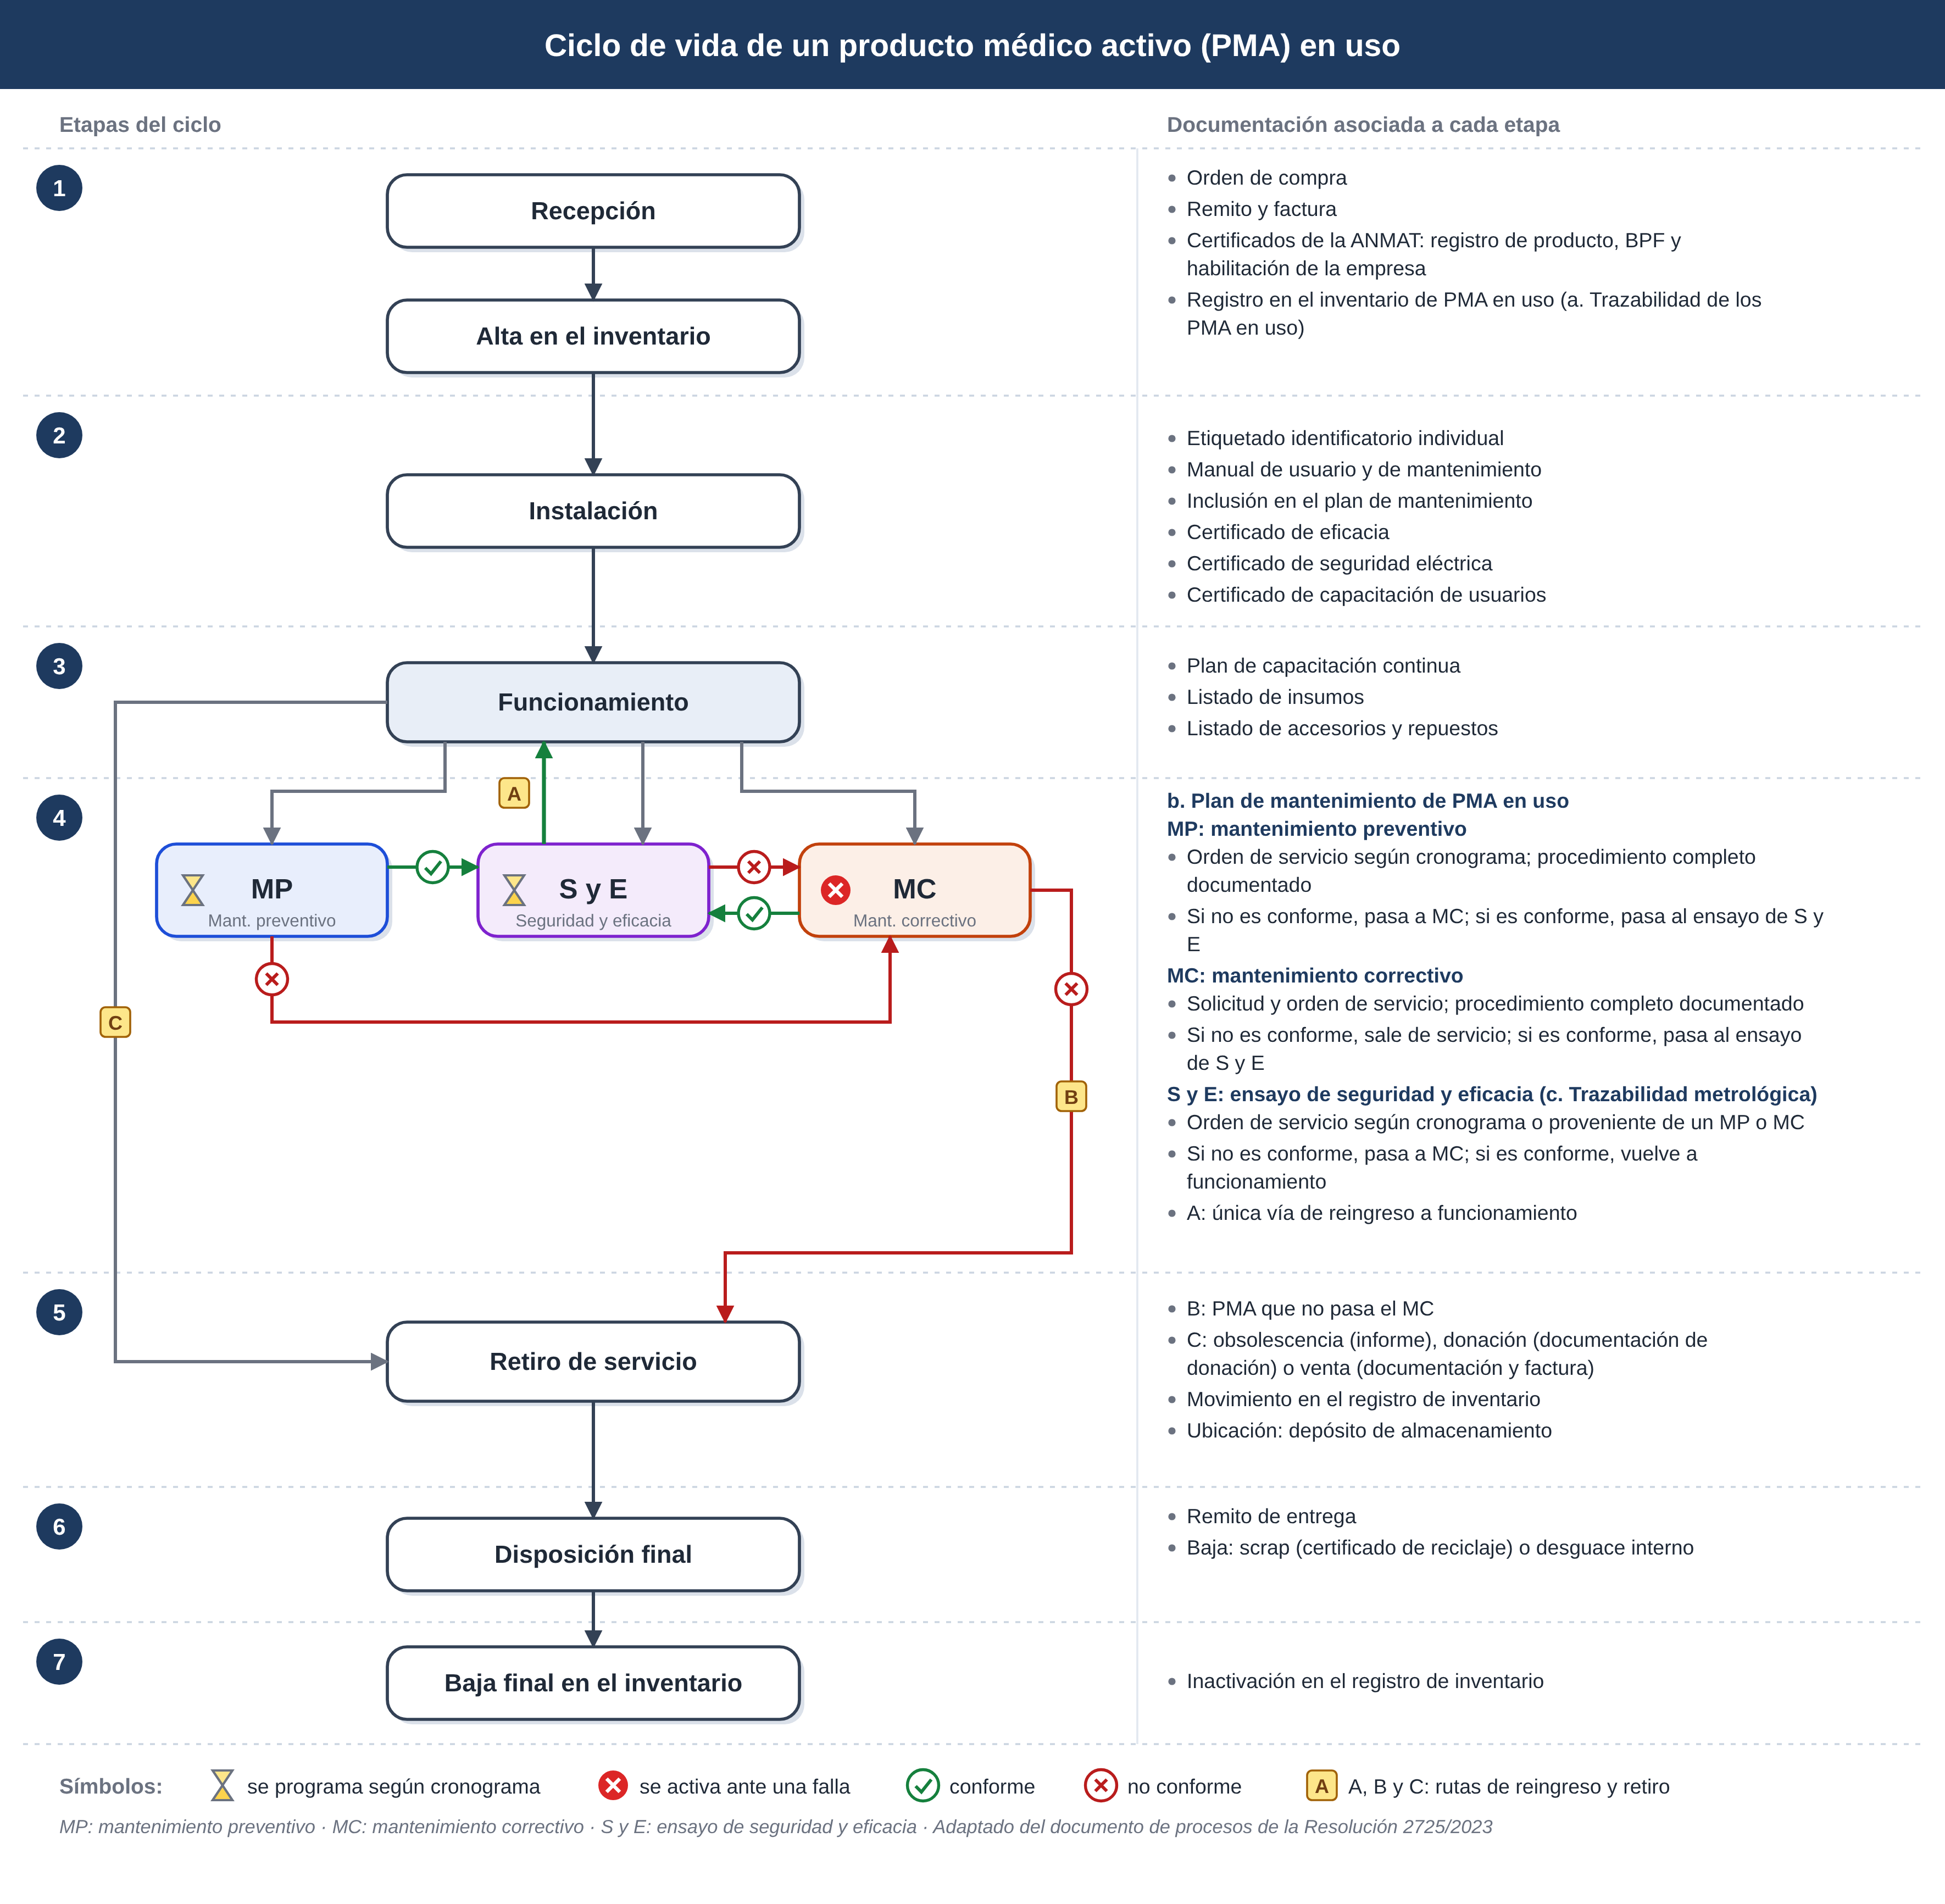
\includegraphics[width=0.85\linewidth]{fotos/figura_ciclo_de_vida_PMA.png}
    \caption[Ciclo de vida de un producto médico activo (PMA).]{Ciclo de vida de un producto médico activo (PMA). Adaptado de \cite{res_2725_2023}.}
    \label{fig:ciclo-vida-pma}
\end{figure}

La norma IRAM 62353:2019, adopción nacional de la IEC 62353, establece los ensayos que deben realizarse sobre un equipo electromédico en uso para evaluar su seguridad \cite{iram_62353}. Comprende una inspección visual, mediciones de seguridad eléctrica como la resistencia de puesta a tierra, la resistencia de aislación y las corrientes de fuga, y un ensayo funcional de las prestaciones del equipo vinculadas a la seguridad. La norma indica además en qué momentos deben realizarse estos ensayos, que son antes de la puesta en servicio, durante el mantenimiento y la inspección, después de una reparación y de forma recurrente, aunque deja en manos de cada institución la definición de los intervalos.

\subsection{Indicadores de gestión del servicio}
\label{sec:indicadores-gestion}
Un plan de mantenimiento que no se mide no permite saber si está funcionando, y por eso el documento de procesos de la Resolución 2725/2023 plantea como uno de sus objetivos que la ejecución del plan se traduzca en informes con indicadores de gestión, de modo que cada planificación aprenda de la anterior \cite{res_2725_2023}. Los indicadores sirven para transformar los registros acumulados en información que permite evaluar el desempeño del servicio y tomar decisiones sobre el parque.

El indicador más directo del plan es el cumplimiento del mantenimiento preventivo, es decir, la proporción de preventivos programados que efectivamente se realizaron en un período. Aunque parece fácil de calcular, depende de cómo se defina qué cuenta como cumplido, porque no es lo mismo considerar cualquier preventivo realizado a que exigir que se haya hecho dentro de la fecha prevista. En este trabajo se adopta el segundo criterio: un preventivo se considera cumplido cuando se realiza dentro del mes para el que fue programado (sección~\ref{sec:estados}).

Sin embargo, desde el punto de vista clínico, lo que más importa no es cuántos preventivos se hicieron sino cuánto tiempo estuvieron los equipos sin poder usarse. El tiempo de inactividad mide justamente eso, y puede obtenerse de dos maneras. La primera es estimarlo como la diferencia entre el momento en que se notifica una falla y el momento en que el equipo vuelve a estar disponible, lo que resulta sencillo pero incluye períodos en los que el equipo puede seguir en funcionamiento, como la demora en tramitar la orden o en cerrarla una vez que el equipo ya volvió a usarse. La segunda es medirlo de manera directa, registrando el inicio y el fin de cada período en que el equipo permanece efectivamente detenido, que es la alternativa adoptada en este trabajo (sección~\ref{sec:estados}). Es el indicador que conecta de manera más directa la gestión del servicio con la atención de los pacientes que se planteaba al comienzo de este trabajo.

A estos se suman dos indicadores clásicos de la ingeniería de mantenimiento. El primero es el tiempo medio entre fallas (MTBF), que mide cuánto tiempo transcurre en promedio entre dos fallas consecutivas de un mismo equipo y es una medida de su confiabilidad. El segundo es el tiempo medio de reparación (MTTR), que mide cuánto se tarda en promedio en resolver una falla, reflejando la capacidad de respuesta del servicio. Analizados junto con la frecuencia y el tipo de fallas de cada equipo, estos indicadores permiten detectar patrones que de otro modo pasarían desapercibidos, como por ejemplo un modelo que falla más que otros de su misma familia, y aportan información concreta para decisiones como el reemplazo de un equipo o la revisión de su plan de mantenimiento. Conviene tener presente que el MTBF solo resulta representativo cuando se cuenta con un historial de fallas suficiente, ya que calculado sobre dos o tres eventos puede dar una imagen engañosa de la confiabilidad real del equipo. Por eso, en SYNAP se calcula como el promedio de días entre fallas consecutivas de un mismo equipo y se presenta siempre junto con la cantidad de fallas en las que se basa (sección~\ref{sec:panel-indicadores}).

Por último, todos estos indicadores comparten una condición, que es que solo son tan confiables como los registros de los que se calculan. Un tiempo de inactividad no puede medirse si no queda registrado cuándo el equipo dejó de estar disponible y cuándo volvió a estarlo, y un MTBF pierde sentido si las fallas de un equipo no están vinculadas a su identificación o aparecen cargadas con descripciones distintas. De esta manera, la calidad de la información que el servicio es capaz de producir depende de las mismas condiciones de trazabilidad y registro desarrolladas a lo largo de este capítulo.


%=======================================================================================================
\newpage
\section{Diseño y desarrollo del sistema}
\label{sec:diseno-desarrollo}

\subsection{Enfoque de trabajo}
\label{sec:enfoque-trabajo}
SYNAP es un prototipo funcional de aplicación web para la gestión de equipamiento médico, desarrollado a partir del servicio de Bioingeniería del Hospital Alemán. El trabajo se planteó como una mejora sobre la gestión actual del parque tecnológico, con una herramienta pensada específicamente para un servicio de Bioingeniería.

El punto de partida fue un relevamiento del servicio, que se desarrolla en la sección~\ref{sec:relevamiento}, orientado a identificar las limitaciones del sistema vigente y a recolectar información de la experiencia de quienes lo usan todos los días. Ese relevamiento incluyó el análisis de las bases con las que el hospital administra su información, donde aparecieron nuevas oportunidades más claras para el sistema, principalmente para evitar errores y omisión de datos. 

Con el problema ya definido, se armó una base de datos propia tomando como punto de partida las del Hospital Alemán y sumando los campos que el servicio debería empezar a registrar para que la aplicación pueda aprovecharlos. El desarrollo del backend se organizó de manera iterativa e incremental, avanzando módulo por módulo, de modo que cada uno quedara funcionando y verificado antes de comenzar con el siguiente. Durante toda esa etapa se trabajó con una base de prueba (sección~\ref{sec:datos-prueba}). A lo largo del proceso se consultó tanto al servicio de Bioingeniería como a docentes con experiencia en el área, para verificar que las decisiones tomadas fueran las adecuadas y para resolver las dudas que fueron apareciendo. 

Para organizar el trabajo entre ambas integrantes se utilizó un repositorio en GitHub, que permitió mantener una única versión del código y llevar registro de cada cambio. Las tareas se repartieron por módulos, dejando siempre para trabajar en conjunto las conexiones entre distintas partes del sistema, y los avances y pendientes se registraron en una planilla compartida para que nada quedara librado a la memoria. A eso se sumó un diagrama de Gantt tentativo, que sirvió para distribuir los tiempos disponibles y seguir el cumplimiento de los objetivos planteados.

\subsection{Relevamiento y requerimientos}
\label{sec:relevamiento}
Antes de definir qué debía hacer el sistema, fue necesario entender cómo trabaja hoy el servicio de Bioingeniería, con qué herramientas y en qué puntos aparecen las principales dificultades. Para eso se combinaron tres fuentes de información. La primera fue la experiencia directa dentro del servicio, ya que una de las integrantes del proyecto se desempeña como pasante en el área y participa de sus tareas cotidianas, desde los mantenimientos preventivos y correctivos hasta la gestión de órdenes de trabajo (OT) en Maximo. La segunda fue una encuesta al personal que utiliza el sistema actual. La tercera fue el análisis de los datos que el servicio registra en Maximo: el histórico de órdenes de trabajo y la base de activos.  A partir de ellas se definieron los perfiles de usuario, los casos de uso y los requerimientos funcionales y no funcionales que guiaron el desarrollo. 

\subsubsection{El servicio de Bioingeniería del Hospital Alemán}
\label{sec:serv-bioing}

El servicio de Bioingeniería del Hospital Alemán fue creado en 2005 para gestionar el ciclo de vida del equipamiento médico de la institución, desde su ingreso hasta su baja definitiva. Depende jerárquicamente de la Dirección Médica y forma parte del área de Facilities Management Services (FMS), que reúne a los sectores responsables de la infraestructura y de los servicios técnicos del hospital. El servicio está a cargo de la jefa de Bioingeniería, Siomara Figueredo. Por debajo de la jefatura se encuentran dos coordinadores, responsables de supervisar el trabajo de los grupos, y el personal técnico, integrado por bioingenieros y técnicos en electromedicina. A este equipo se suman una pasante y un administrativo.

La Figura~\ref{fig:organigrama} muestra la organización del servicio: el primer coordinador supervisa los grupos 1 y 2, y el segundo los grupos 3, 4 y 5. 

\begin{figure}[H]
    \centering
    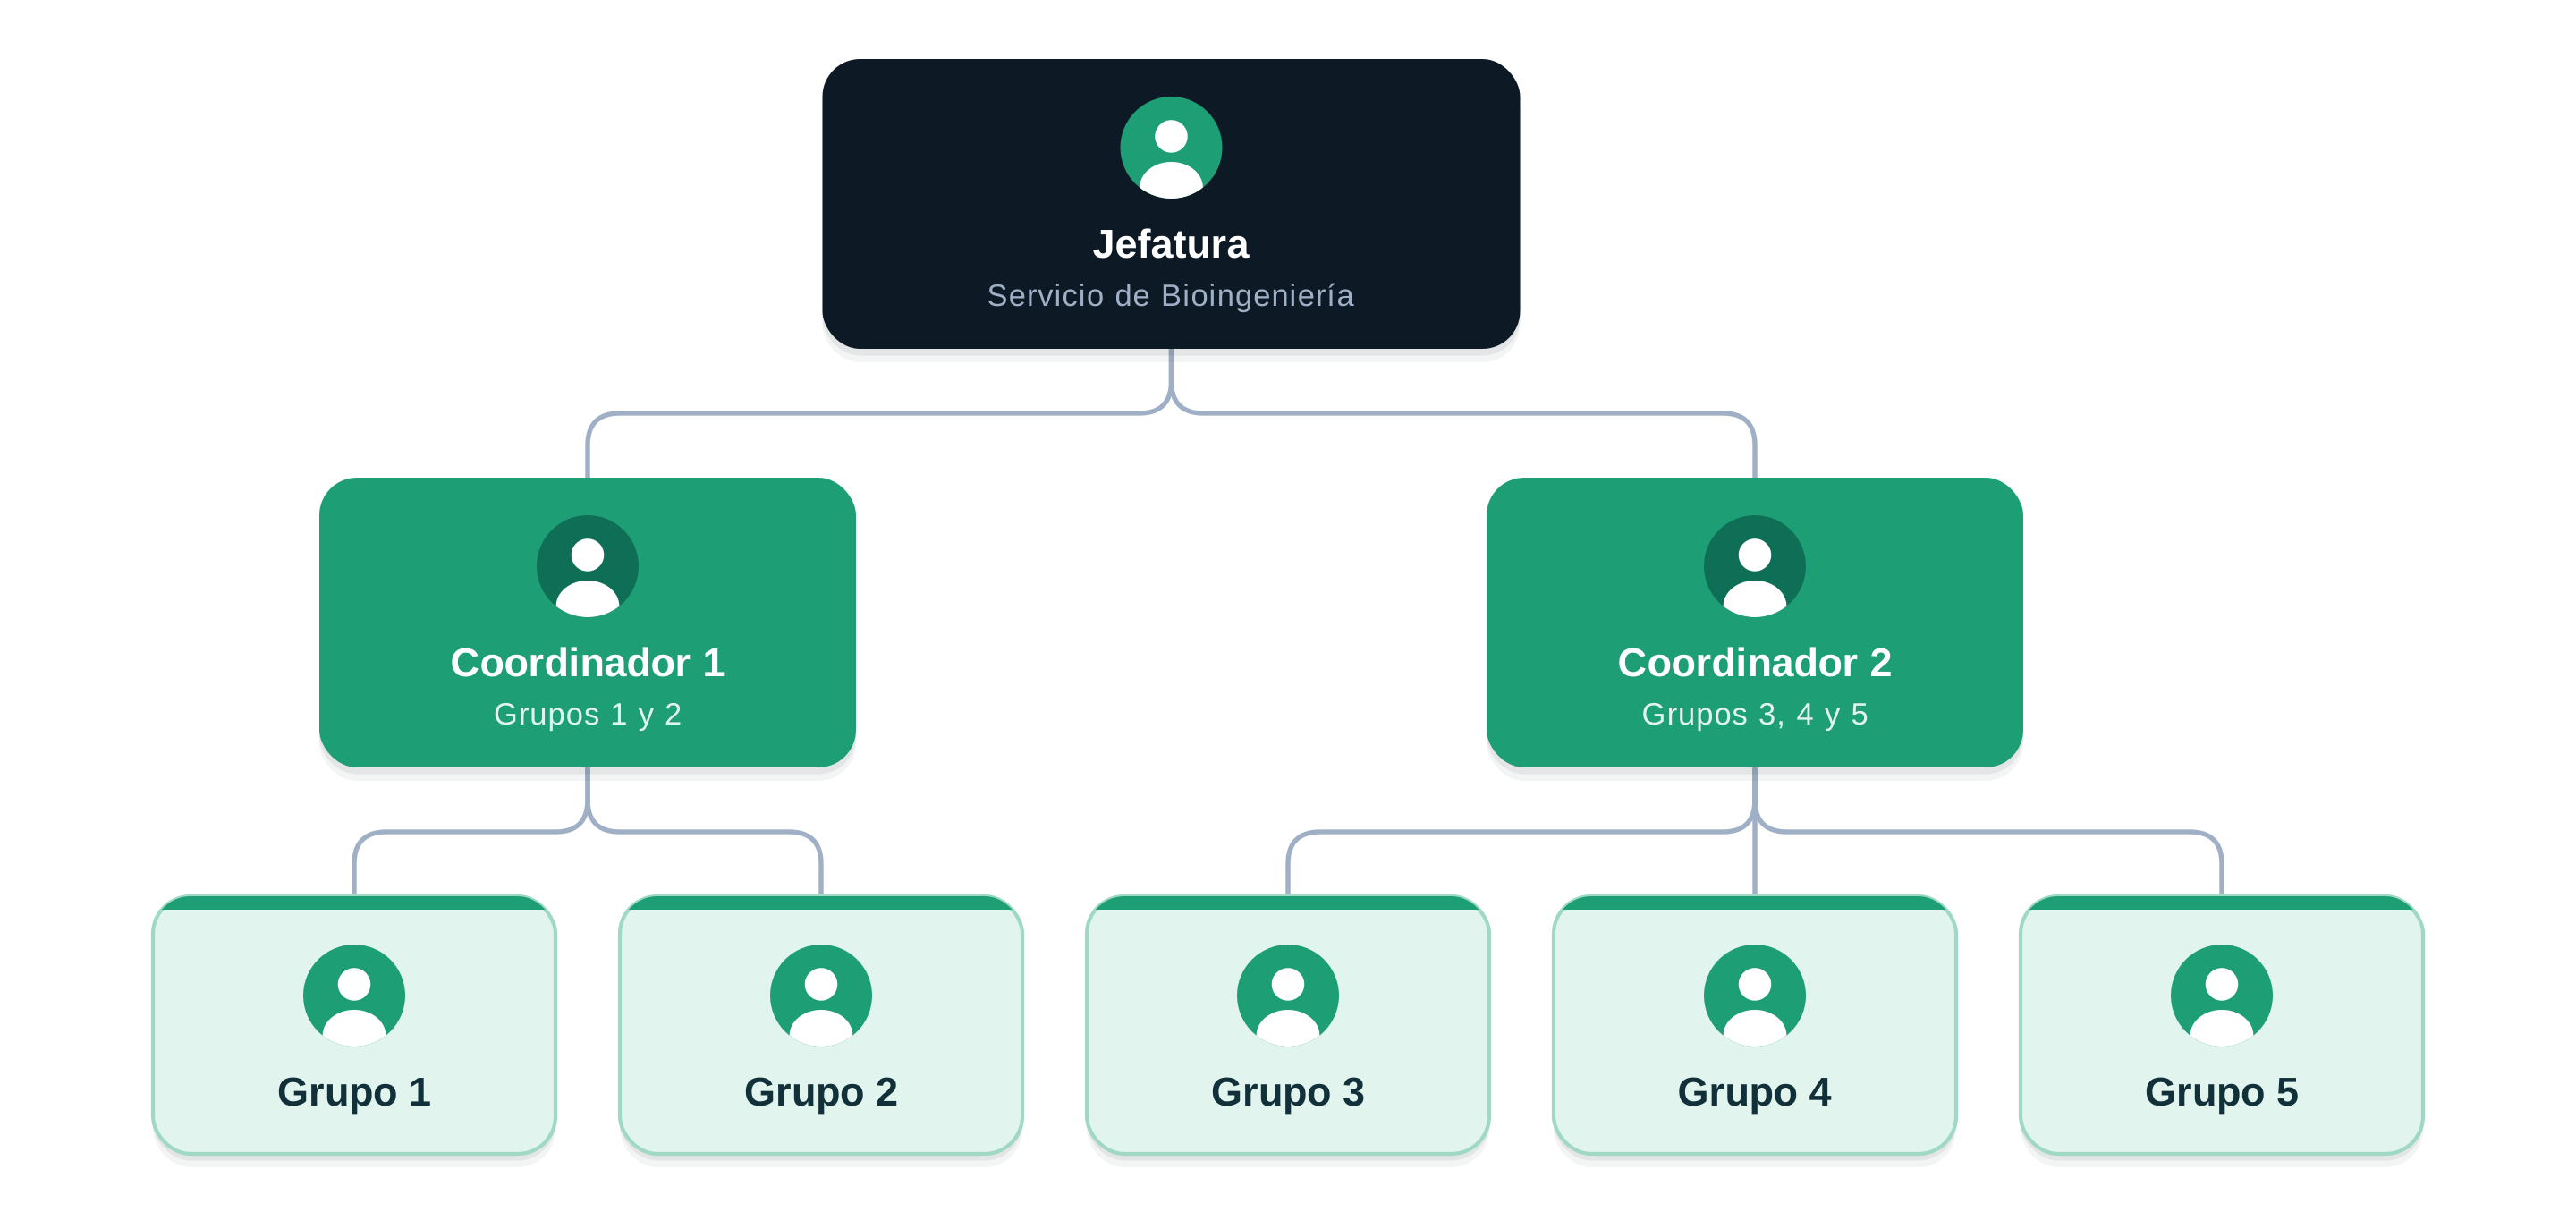
\includegraphics[width=0.9\linewidth]{fotos/Figura_4_1_organigrama.png}
    \caption[Organigrama del servicio de Bioingeniería del Hospital Alemán.]{Organigrama del servicio de Bioingeniería del Hospital Alemán. Elaboración propia.}
    \label{fig:organigrama}
\end{figure}

El trabajo se organiza en siete grupos, cada uno responsable de un conjunto de áreas del hospital o de un tipo de equipamiento:
\begin{itemize}
    \item Grupo 1 (tres integrantes): quirófanos centrales y ambulatorios, endoscopía, litotricia y salas de partos.
    \item Grupo 2 (dos integrantes): terapias intensivas e intermedias, unidad coronaria, pediatría, neonatología, emergencias y esterilización.
    \item Grupo 3 (dos integrantes): diagnóstico por imágenes y radioterapia.
    \item Grupo 4 (dos integrantes): laboratorio e investigación.
    \item Grupo 5 (dos integrantes): policlínica, hospital de día y consultorios externos.
    \item Grupo 6: bombas de infusión.
    \item Grupo 7: instrumental quirúrgico.
\end{itemize}
Los grupos 6 y 7 existen como grupos propios dentro de la organización del servicio y del sistema de gestión, pero no tienen personal exclusivo. El Grupo 6 está a cargo de una bioingeniera del Grupo 4 y el Grupo 7 de una bioingeniera del Grupo 1. Por eso, la carga de trabajo real de cada persona no depende solo del grupo al que pertenece, sino también de estas responsabilidades adicionales. Si bien los grupos tienen áreas definidas, existe además una colaboración continua entre ellos, dado que muchos equipos son transversales y requieren procedimientos comunes de control y verificación.

Toda la actividad del servicio se registra en IBM Maximo, que concentra el inventario de activos, las solicitudes de servicio, las órdenes de trabajo y los planes de mantenimiento preventivo. En el caso de los preventivos, el sistema genera automáticamente el primer día de cada mes las órdenes de trabajo de los equipos que tienen un mantenimiento programado, según el plan asignado a cada activo. Sin embargo, como Maximo no permite visualizar con claridad los preventivos de los meses siguientes, cada grupo lleva además una planilla propia donde anticipa los equipos que van a vencer y aquellos que requieren emitir una orden de compra con anticipación. Los mantenimientos pueden realizarse de forma interna o estar tercerizados. En este último caso se agrega un circuito administrativo de presupuestos, firmas, requisiciones y órdenes de compra que se sigue por fuera del sistema. Una vez realizado el mantenimiento, la orden se completa en Maximo, se imprime junto con la planilla interna o el informe del proveedor y se entrega al coordinador del grupo. El coordinador revisa lo realizado, sella el documento y lo archiva en la carpeta física del equipo. Finalmente, se coloca en el equipo una etiqueta amarilla con la fecha de realización, el vencimiento y el responsable.

Los correctivos, en cambio, se originan en una falla detectada por el personal de los servicios clínicos. La vía formal es la carga de una solicitud de servicio en Maximo, que aparece en la bandeja de entrada de Bioingeniería. En la práctica, los servicios suelen avisar además por teléfono para acelerar la respuesta. En situaciones urgentes se acude directamente al servicio y se pide que la solicitud se cargue después de resuelto el problema, de manera que el registro queda supeditado a que alguien lo complete a posteriori. En estos casos, la fecha que queda registrada no necesariamente refleja el momento en que realmente se detectó la falla. Las solicitudes son asignadas por los coordinadores o la jefatura, ya que el personal técnico no puede autoasignarse órdenes de trabajo. Cuando durante un preventivo se detecta una falla, Maximo permite generar una orden correctiva asociada que queda vinculada a la intervención original. Al cierre, la orden correctiva se imprime, la firma el servicio y el coordinador la valida antes de archivarla.

Este recorrido muestra que una parte importante del proceso ocurre por fuera del sistema de gestión: las planillas de cada grupo, los avisos telefónicos, las firmas en papel y los circuitos de compras. La consecuencia es que la información de un mismo equipo queda repartida entre varios soportes. Como se planteó en la sección~\ref{sec:indicadores-gestion}, esa dispersión afecta directamente la posibilidad de calcular indicadores confiables.

Cada equipo del parque lleva hoy dos etiquetas (Figura~\ref{fig:etiquetas-qr}). La de identificación muestra el código de activo acompañado de un código de barras y un código QR, aunque este último no se utiliza, ya que ninguno de los sistemas del servicio lo lee. La de mantenimiento preventivo indica el mes en que se hizo el último control, el del próximo y quién lo realizó, y funciona como recordatorio a la vista de cualquiera que use el equipo. Ese QR, ya colocado en todo el parque, es el que SYNAP aprovecha para acceder a la información de cada equipo desde el celular (apartado~\ref{sec:activos-qr}).

\begin{figure}[H]
    \centering
    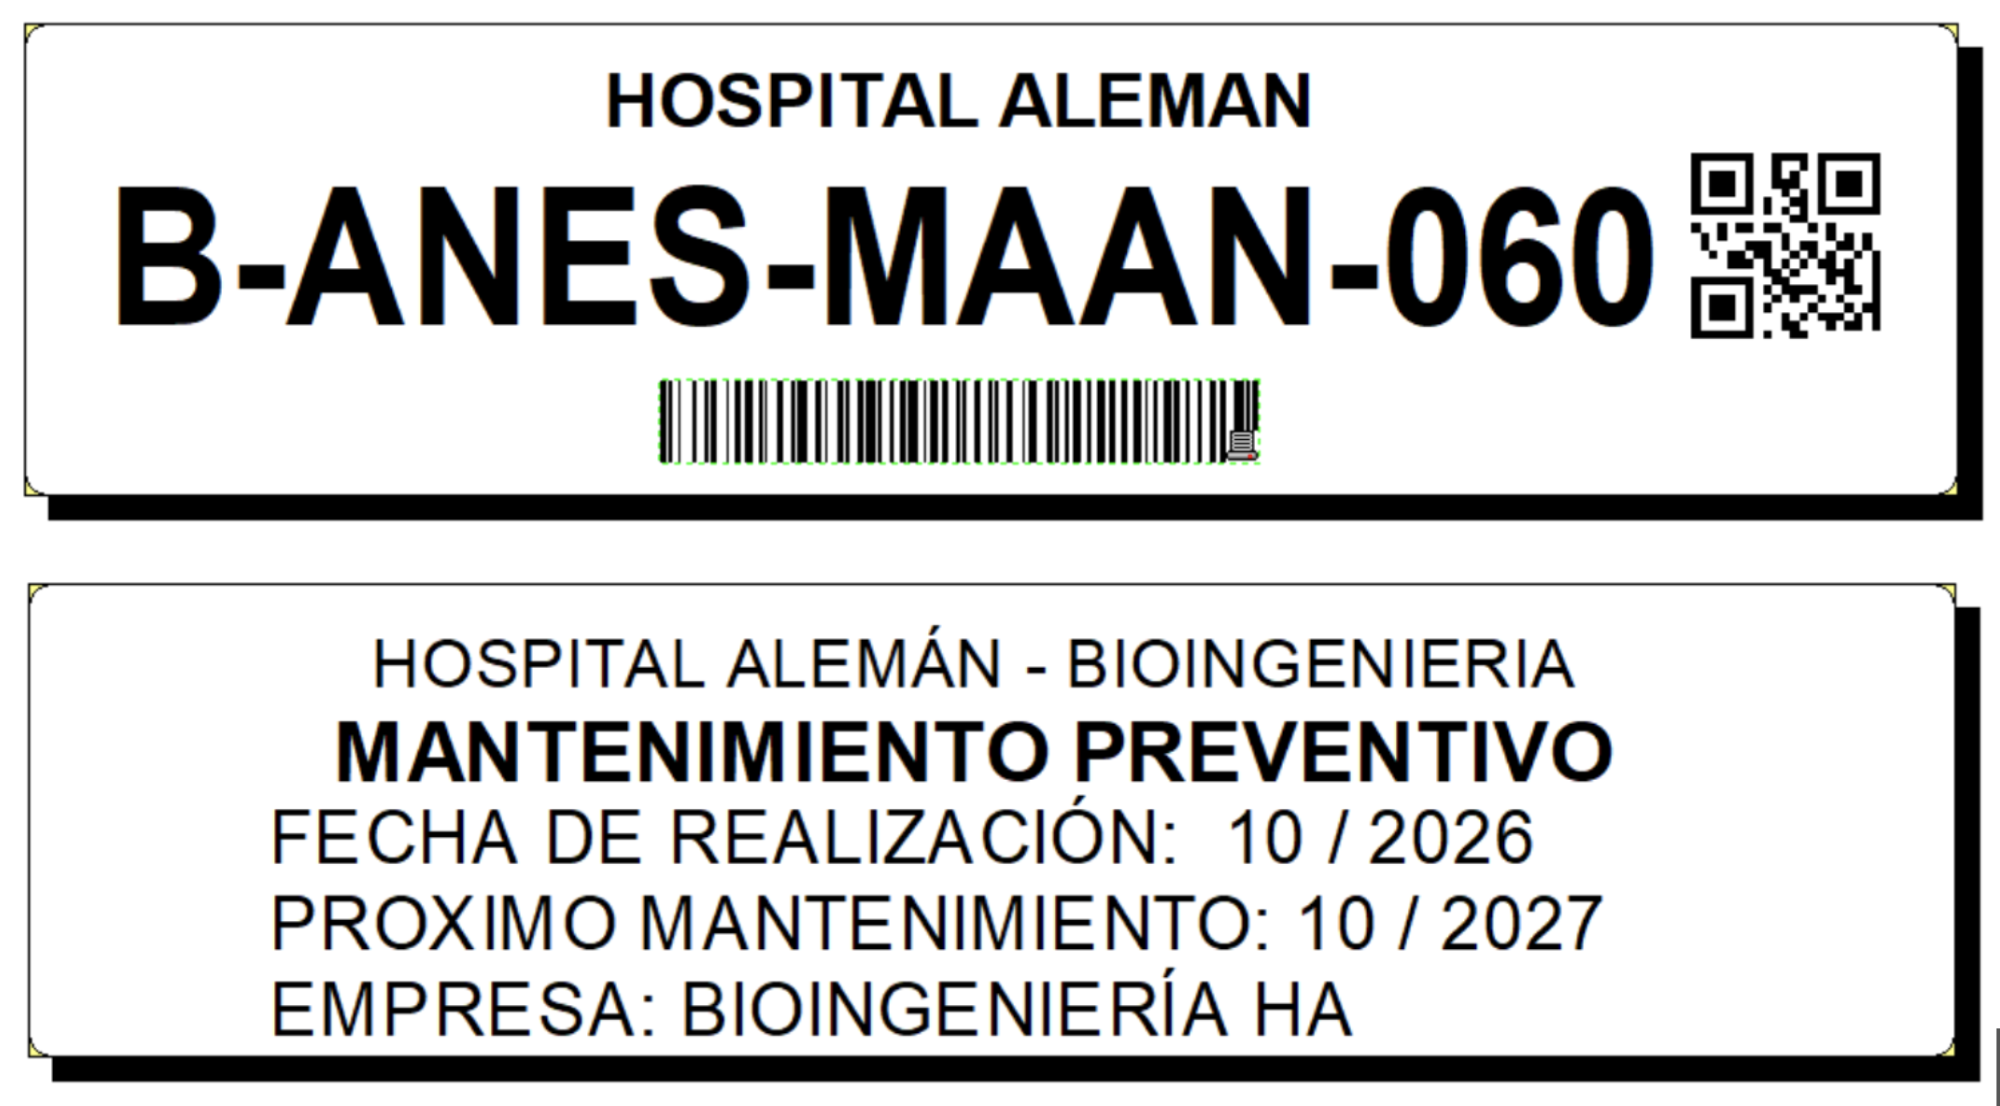
\includegraphics[width=0.6\linewidth]{fotos/etiquetas}
    \caption[Etiquetas de identificación y de mantenimiento preventivo de los equipos.]{Etiquetas de identificación (arriba) y de mantenimiento preventivo (abajo) colocadas en los equipos del Hospital Alemán. Fotografía propia.}
    \label{fig:etiquetas-qr}
\end{figure}

\subsubsection{Encuesta}
\label{sec:encuesta}

Para conocer la experiencia de quienes usan el sistema todos los días, se realizó una encuesta mediante un formulario en línea, respondida entre el 5 y el 18 de mayo de 2026. Participaron ocho integrantes del servicio: dos coordinadores, tres bioingenieros y tres técnicos, de un total de 16 personas que conforman el área. El formulario combinó preguntas cerradas, algunas de ellas con escala de 1 a 5, y preguntas abiertas. Se organizó en cinco bloques: el uso actual del sistema y su valoración, las dificultades y problemas concretos, las funcionalidades deseadas (acceso móvil, códigos QR, reporte de fallas y notificaciones), los indicadores de gestión y, por último, un espacio para comentarios libres. Las respuestas abiertas se analizaron agrupándolas por temas recurrentes. El cuestionario y los resultados de las preguntas cerradas se incluyen en el \ref{anexo:encuesta}.

La totalidad de los encuestados utiliza Maximo varias veces por día, lo que confirma que el sistema de gestión es una herramienta central en la rutina del servicio y no un registro accesorio. Aun así, la valoración que recibe es baja. Sobre una escala de 1 a 5, la facilidad de uso obtuvo un promedio de 3,0, la completitud de la información un 2,6 y la eficiencia para el trabajo diario un 2,5. La mitad de los encuestados calificó la eficiencia con 1 o 2 y los más señalados fueron los siguientes (Tabla~\ref{tab:problemas-eficiencia}):

\begin{table}[H]
    \caption{Problemas de eficiencia más señalados por el personal encuestado.}
    \label{tab:problemas-eficiencia}
    \centering
    \begin{tabular}{lc}
        \toprule
        \textbf{Problema señalado} & \textbf{Respuestas} \\
        \midrule
        Falta de automatización & 6 de 8 \\
        Dificultad para registrar fallas & 6 de 8 \\
        Datos no normalizados & 5 de 8 \\
        Falta de actualización de los datos & 5 de 8 \\
        Información redundante o repetida & 4 de 8 \\
        Dificultad para encontrar información del equipo & 2 de 8 \\
        \bottomrule
    \end{tabular}
\end{table}

Las respuestas abiertas permitieron darle contenido concreto a esas categorías. El tema más repetido fue la generación de informes y reportes, mencionada en seis de las ocho respuestas, ya sea por la dificultad para obtenerlos o por la demora para imprimirlos. Cuatro encuestados señalaron además la lentitud del sistema y la cantidad de pasos y ventanas que requiere completar una tarea sencilla. Una de las coordinadoras describió que, cuando necesita información específica, filtra en Maximo hasta donde el sistema lo permite, exporta el resultado y continúa trabajando en una planilla aparte. Según su respuesta, todo lo que el sistema no resuelve termina haciéndose por fuera, con información duplicada y el doble de trabajo. La misma respuesta señala que Maximo tiene muchos campos que al servicio no le sirven por tratarse de un programa genérico pensado para la industria. Esto confirma, desde la experiencia de los propios usuarios, el desajuste planteado en la sección~\ref{sec:contexto-problema}.

Además, la encuesta relevó necesidades puntuales que se tradujeron en requerimientos: registrar los repuestos utilizados y los accesorios entregados, y vincularlos con el circuito de compras (cuatro respuestas); filtrar mejor la información (tres); adjuntar archivos a las órdenes de trabajo (dos); y contar con un semáforo de vencimientos y un aviso para los activos sin protocolo de mantenimiento, con protocolos definidos según el tipo de equipo y su riesgo (una bioingeniera). Una coordinadora pidió también que el sistema no permita repetir ni armar mal el identificador de un equipo.

Las funcionalidades propuestas tuvieron buena recepción. El acceso desde el celular sin instalar una aplicación obtuvo un promedio de 4,5 y la identificación por código QR, 4,4. Al escanear un equipo, lo más esperado era reportar fallas (6 respuestas), acceder a los manuales (5) y consultar el historial de mantenimiento (4). Una coordinadora observó que esto depende de quién escanea: al usuario del servicio clínico le interesa reportar una falla, mientras que a Bioingeniería le interesa ver el historial y el stock de accesorios, lo que fue determinante para el diseño. Siete de los ocho encuestados consideraron importante reportar fallas desde el sistema y seis, contar con un panel de indicadores, donde los más mencionados fueron el cumplimiento de los preventivos, las fallas por equipo y los tiempos de reparación y fuera de servicio. Las notificaciones por correo dividieron las opiniones (cuatro a favor y cuatro en contra), por lo que se las consideró complementarias.

En conjunto, la encuesta mostró que las dificultades del servicio no se deben a la falta de un sistema, sino a que el sistema disponible no acompaña la forma en que el servicio trabaja. Cada hallazgo se tradujo en uno o más requerimientos (secciones~\ref{sec:requerimientos-funcionales} y~\ref{sec:requerimientos-no-funcionales}). Pedidos como la tecnovigilancia o la integración con compras exceden el alcance y se retoman en las perspectivas futuras.

\subsubsection{Análisis exploratorio de los datos de IBM Maximo}
\label{sec:analisis-maximo}
Para complementar la encuesta con evidencia de los propios registros, se analizaron dos exportaciones de Maximo provistas por el servicio: el inventario de activos y el histórico de órdenes de trabajo. Como se trata de información real de la institución, el análisis se hizo sobre valores agregados, sin utilizar datos que identifiquen a personas.

\noindent\textbf {Base de activos}

El inventario reúne 6.302 registros, de los cuales cerca de 4.000 corresponden a equipos en uso. Se identificaron los siguientes problemas:
\begin{itemize}
    \item Códigos mal construidos: Maximo impide repetir un código, pero no controla su formato, y se encontraron 26 códigos con errores de tipeo, como espacios, puntos o guiones de más.
    \item Registros que no son equipos: 120 activos son entradas genéricas, como los “pedidos a Bioingeniería” de cada servicio, creadas para canalizar pedidos que no se refieren a un equipo identificado.
    \item Ubicación: el área del código no indica dónde está el equipo, y uno de cada cinco equipos activos no tiene ubicación cargada.
    \item Descripciones sin normalizar: los oxímetros de pulso, por ejemplo, figuran con 21 descripciones distintas, y en un cuarto de los registros la descripción incluye el estado del equipo.
    \item Datos faltantes: el 9\% de los activos no tiene un número de serie utilizable y casi un tercio de los equipos activos tiene al menos un campo vacío.
\end{itemize}
\textbf {Histórico de órdenes de trabajo}

Reúne 57.065 órdenes registradas entre agosto de 2015 y septiembre de 2026, unas 5.000 por año. Los problemas identificados fueron:

\begin{itemize}
    \item No se distingue el tipo de orden: la exportación no incluye un campo que indique si es preventiva o correctiva, por lo que se lo dedujo a partir de la descripción y del origen. Con esa clasificación, más de la mitad de las órdenes son preventivas y alrededor de un tercio, correctivas.
    \item Estados superpuestos: el campo admite nueve valores, y tres de ellos son formas de dar una orden por finalizada.
    \item Fechas poco confiables: más de la mitad de las órdenes finalizadas se cerraron en lotes, de modo que la fecha de cierre no refleja cuándo se hizo el trabajo, y la fecha de cumplimiento está vacía en la mayoría de las correctivas.
    \item Sin tiempo fuera de servicio: ningún campo indica cuándo un equipo dejó de estar disponible ni cuándo volvió a estarlo.
    \item Fallas sin equipo: el 34\% de las correctivas se cargó sobre los registros genéricos, por lo que esas fallas no forman parte del historial de ningún equipo.
    \item Descripciones que no informan la falla: casi la mitad de las correctivas se describe con una o dos palabras, como “bomba” o “monitor”, y la descripción se usa también para anotar novedades, a falta de un lugar donde registrar el avance de la intervención.
    \item Prioridad sin uso: el campo está vacío en prácticamente todas las órdenes.
\end{itemize}
\textbf {Consecuencias para la gestión}

Con estos registros no es posible calcular de manera confiable la mayoría de los indicadores de la sección~\ref{sec:indicadores-gestion}. El tiempo de inactividad y el tiempo medio de reparación no pueden obtenerse, y el cumplimiento del mantenimiento preventivo y el tiempo medio entre fallas solo pueden estimarse. El problema, entonces, no es la falta de registros, ya que en once años se acumularon más de 57.000 órdenes, sino que esos registros no capturan los datos necesarios para evaluar la gestión, y los que sí capturan no están normalizados.

\subsubsection{Perfiles de usuario}
\label{sec:perfiles-usuario}
A partir del relevamiento se definieron cuatro perfiles de usuario. Cada persona que accede a SYNAP tiene asignado uno, y ese perfil determina qué pantallas ve y qué acciones puede realizar. El control se aplica en el backend, como se detalla en la sección~\ref{sec:backend-bd}. La definición de los perfiles retoma la distinción que establece el documento de procesos de la Resolución 2725/2023 entre quienes gestionan el cumplimiento del plan de mantenimiento y quienes lo ejecutan \cite{res_2725_2023}, y suma el personal asistencial, que detecta y reporta las fallas, y la jefatura del servicio, que necesita una visión global del área. Los perfiles se presentan en el orden en que intervienen a lo largo del recorrido de una falla, desde su detección hasta la evaluación del desempeño del servicio.

\textbf {Enfermería.} Representa al personal asistencial de los servicios clínicos, enfermeros y médicos, que utiliza el equipamiento en la atención de los pacientes y suele ser el primero en detectar una falla. Reporta en medio de un turno o de un procedimiento y tiene poco conocimiento técnico de los equipos, por lo que su recorrido se redujo a lo indispensable: escanear el código QR del equipo o ingresar su identificador, indicar la falla y la ubicación, y seguir el estado de la solicitud enviada. Si el problema no corresponde a un equipo médico, puede describirlo sin asociarlo a un activo. No tiene acceso al inventario, a las órdenes de trabajo ni al stock, ya que no los necesita para su tarea.

\textbf {Técnico.} Corresponde a los bioingenieros y técnicos en electromedicina que integran los grupos del servicio y ejecutan los mantenimientos. Cada técnico pertenece a un grupo y trabaja sobre las órdenes de ese grupo: toma las que están sin asignar, las reasigna a un compañero, registra el avance en la bitácora, completa el checklist de los preventivos, registra los insumos consumidos y cierra las órdenes. Además puede consultar la ficha y el historial de cualquier equipo, dar de alta equipos nuevos y consultar el stock.

\textbf {Coordinación.} Gestiona uno o más grupos y es responsable de que el trabajo se distribuya y se cumpla. Recibe las solicitudes de sus grupos y decide si aceptarlas, rechazarlas indicando el motivo o corregirlas antes de convertirlas en una orden de trabajo, que puede asignar a un técnico o dejar disponible para el grupo. Define los planes de mantenimiento preventivo y sus checklists, administra los catálogos de tipos de equipo, da de alta insumos y gestiona las compras. También revisa las órdenes preventivas completadas, y autoriza su cierre o las devuelve para que se corrijan.

\textbf {Jefatura.} Corresponde a la jefatura del servicio, que necesita una visión global del área sin restricción por grupo. Su herramienta principal es el panel de indicadores, que le permite evaluar el desempeño del servicio y fundamentar decisiones sobre el parque, como el recambio de un equipo o la revisión de un plan de mantenimiento. Puede consultar toda la información del sistema, incluidas las órdenes de trabajo de todos los grupos, que ve en modo de solo lectura, ya que supervisa el trabajo pero no lo ejecuta.

\subsubsection{Casos de uso}
\label{sec:casos-uso}

Los casos de uso describen las interacciones concretas que cada perfil realiza con el sistema para cumplir un objetivo. Se definieron a partir de los procesos relevados en la sección~\ref{sec:serv-bioing} y de las necesidades expresadas en la encuesta. Algunos pueden ser realizados por más de un perfil, y en ellos el alcance de cada uno no es el mismo. El caso más claro son las órdenes de trabajo: el técnico solo opera sobre las de su grupo y la coordinación sobre las de los grupos que coordina, mientras que la jefatura puede consultarlas todas, pero no modificarlas. 

Para facilitar su lectura, los casos de uso se representan en tres diagramas, uno por cada módulo del sistema. El primero reúne las solicitudes de servicio y las órdenes de trabajo (Figura~\ref{fig:caso-1}), el segundo los activos y el mantenimiento preventivo (Figura~\ref{fig:caso-2}) y el tercero el stock y los indicadores (Figura~\ref{fig:caso-3}). En el primer diagrama, los casos se agrupan además según la etapa del circuito a la que pertenecen, desde el reporte de la falla hasta la ejecución del mantenimiento, de modo que el diagrama puede leerse de arriba hacia abajo siguiendo el recorrido de una orden. 

Los casos comunes a todos los perfiles, como el inicio de sesión y el escaneo de un equipo, se asocian a un actor general denominado Usuario, del que heredan los cuatro perfiles. La relación «extend» señala un caso que se agrega de forma opcional a otro, como la generación de una correctiva durante el checklist de un preventivo. El segundo diagrama incluye además un actor que no corresponde a un perfil sino al propio sistema: una tarea programada que genera cada mes las órdenes de mantenimiento preventivo sin intervención del personal.

\begin{figure}[H]
    \centering
    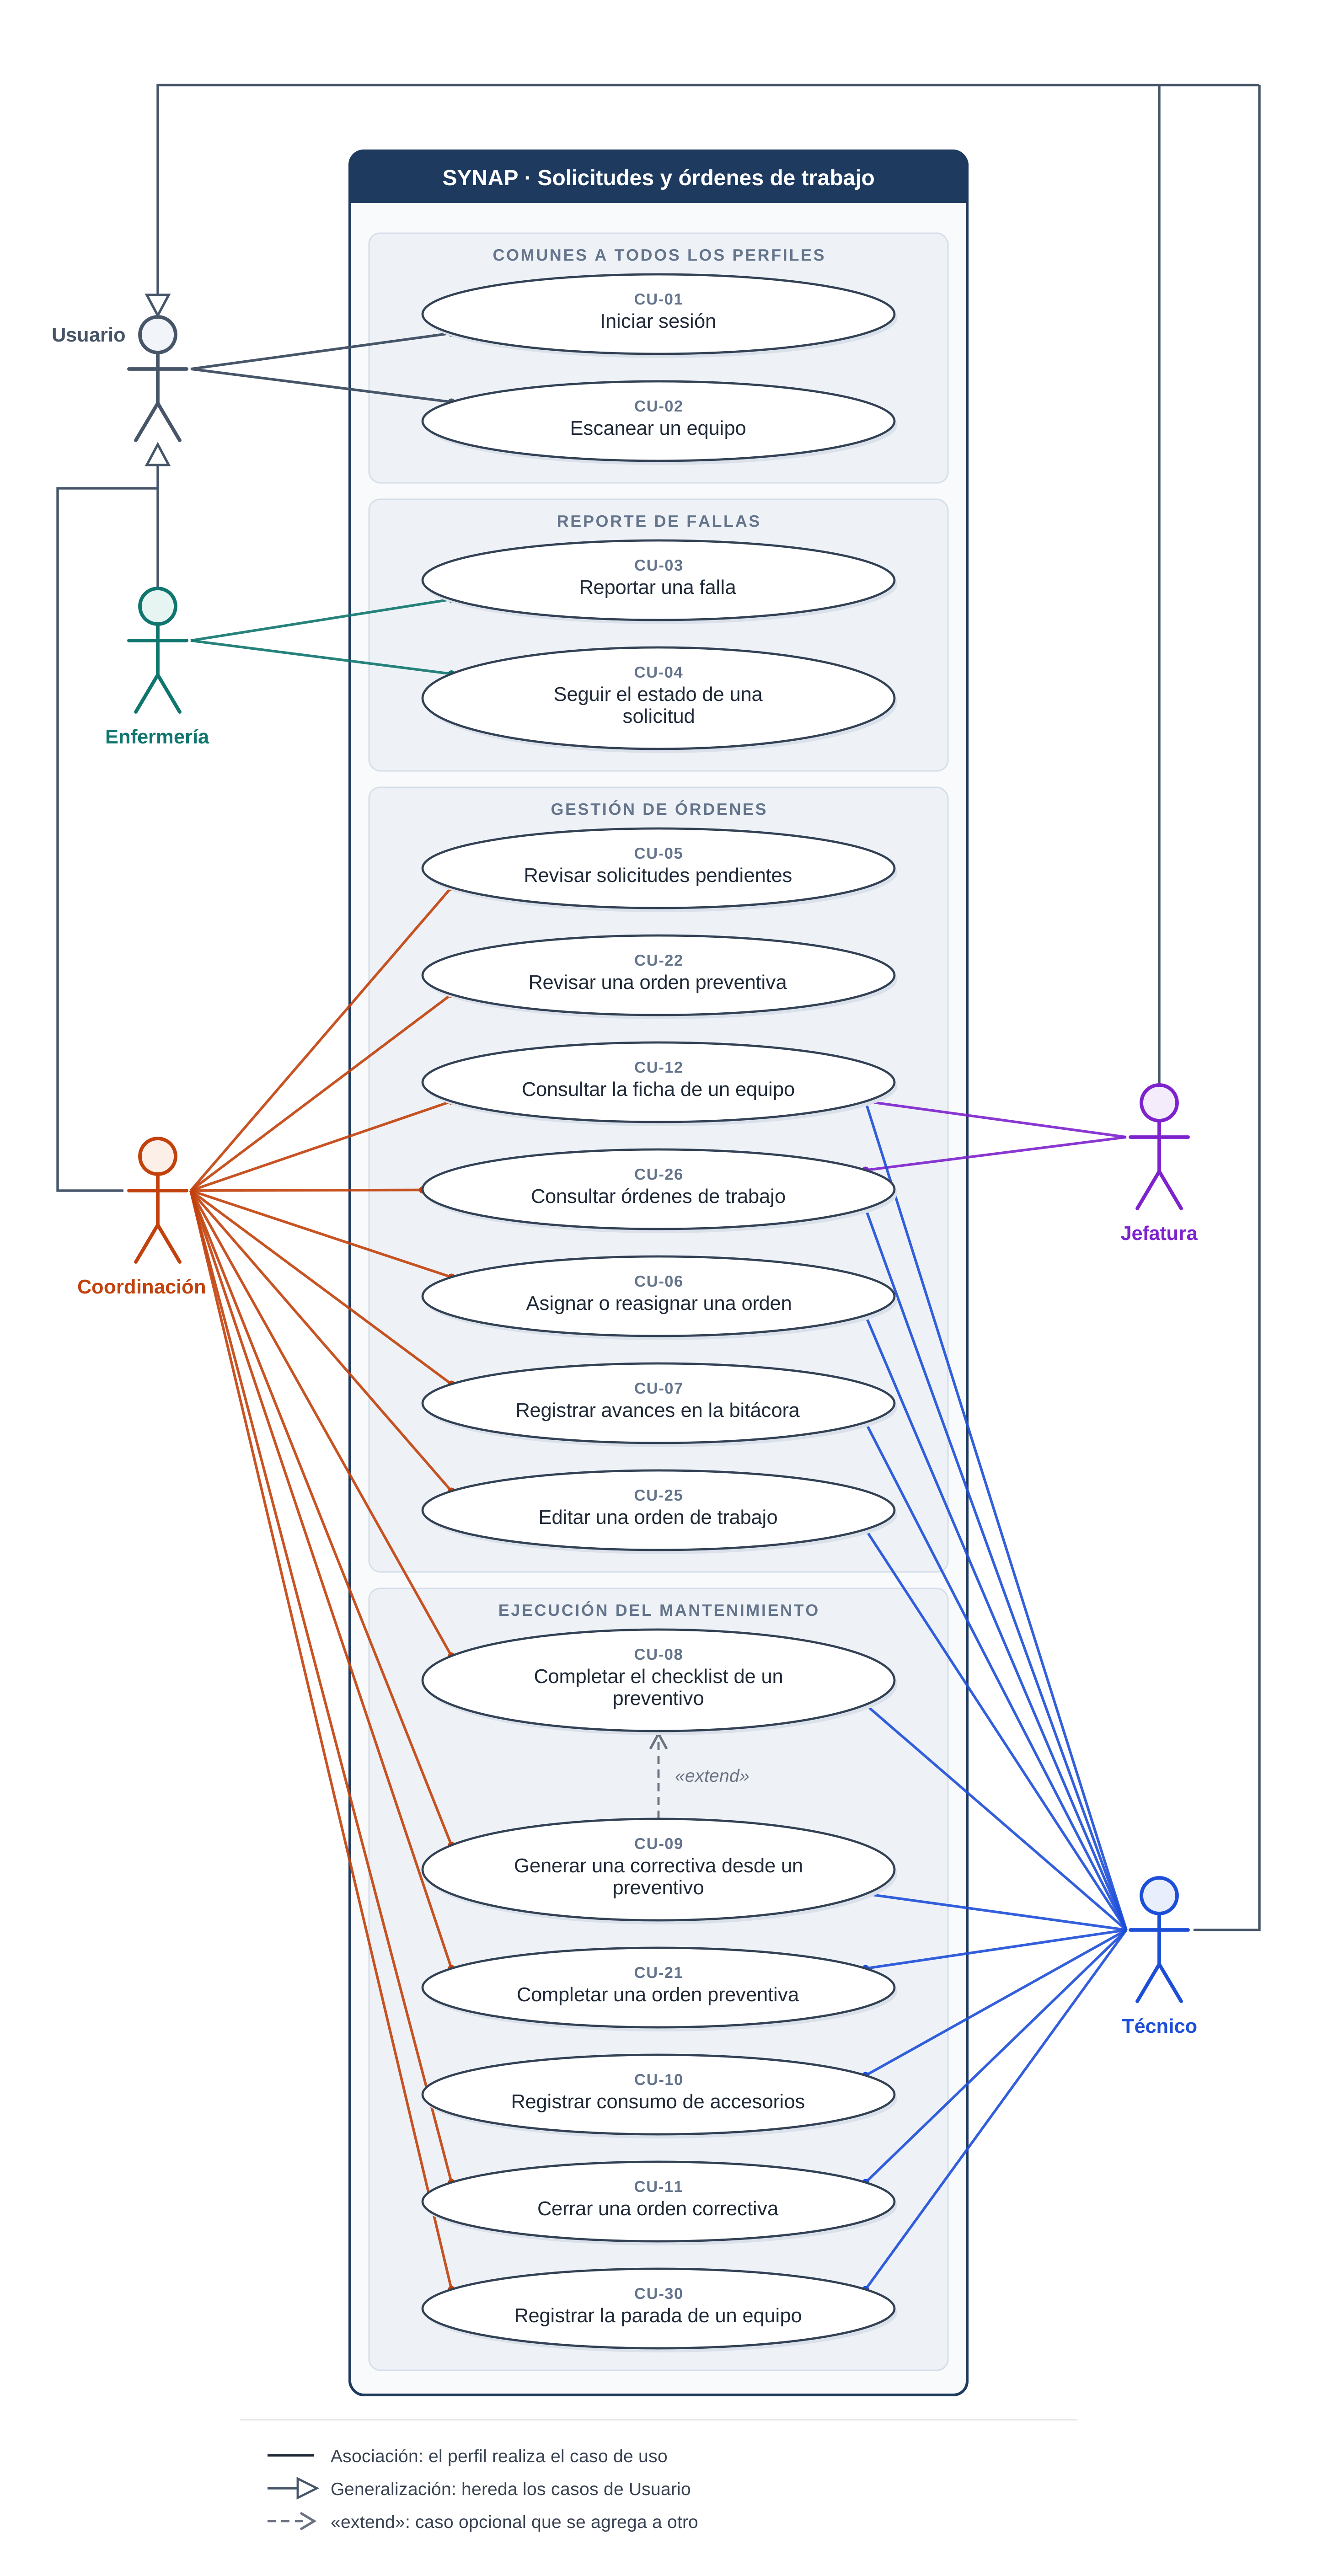
\includegraphics[width=0.6\linewidth]{fotos/Figura_4_2_casos_de_uso_solicitudes_y_ordenes.png}
    \caption{Diagrama de casos de uso del módulo de solicitudes y órdenes de trabajo.}
    \label{fig:caso-1}
\end{figure}

\begin{figure}[H]
    \centering
    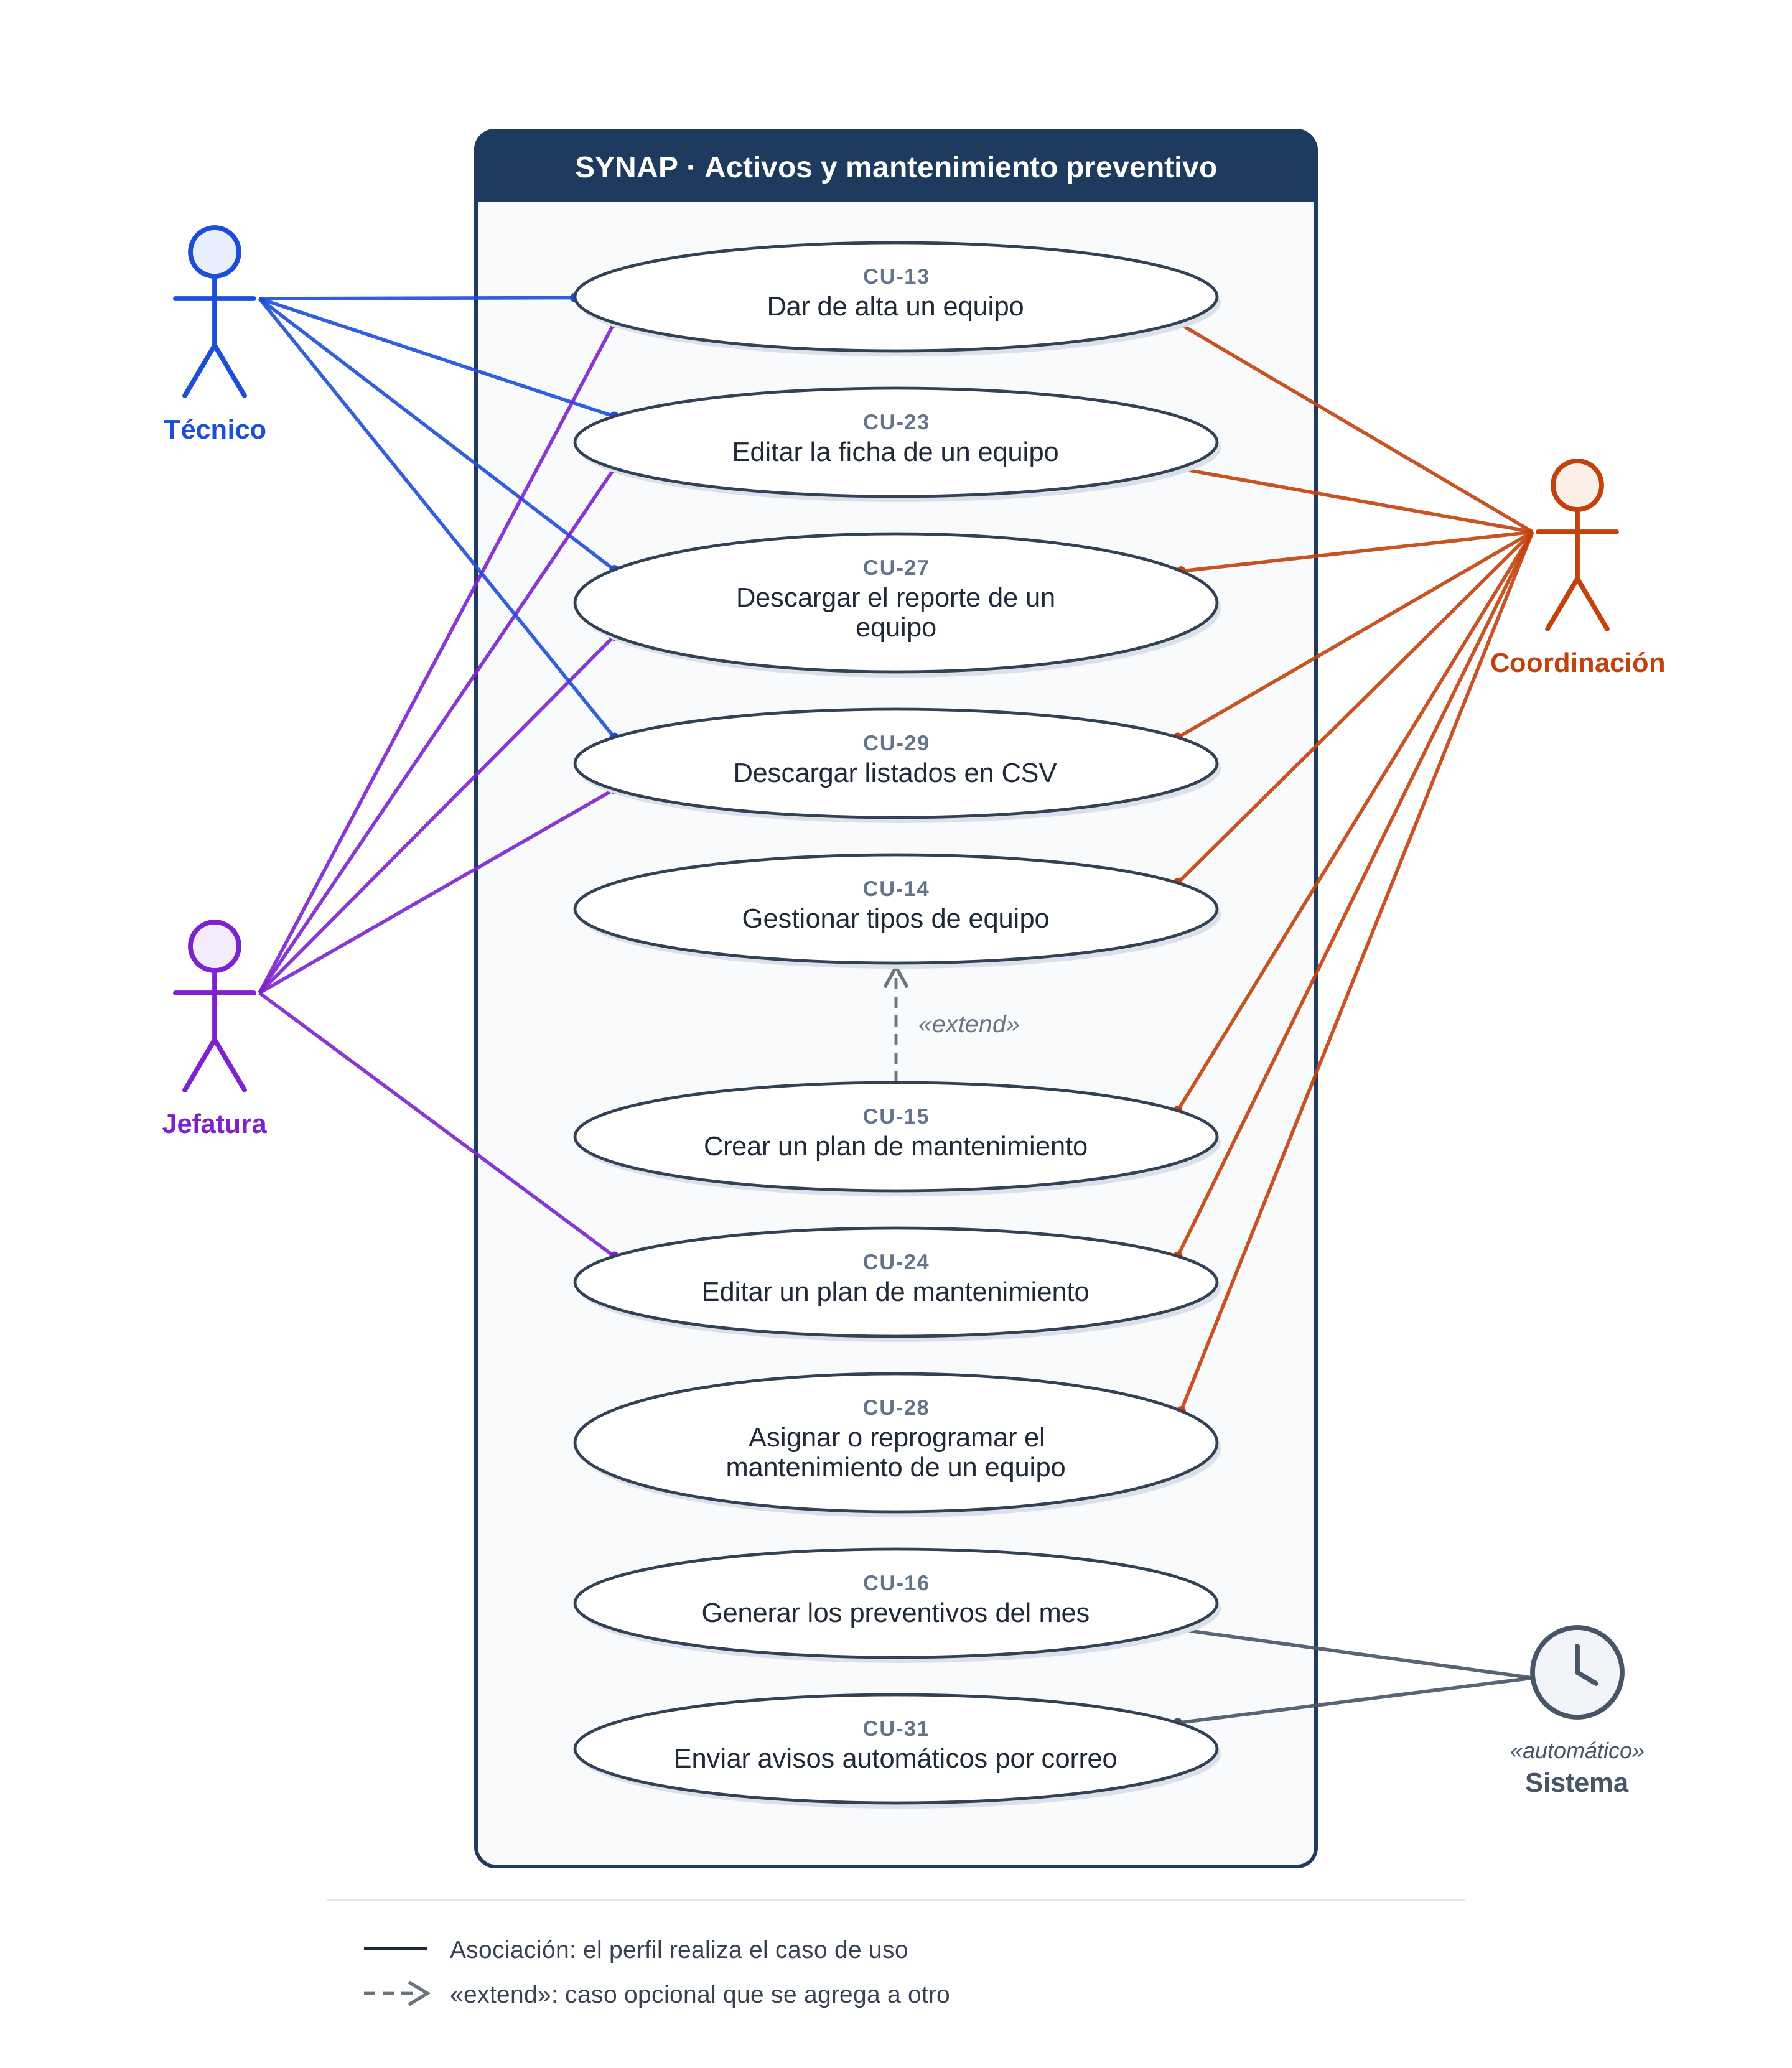
\includegraphics[width=0.9\linewidth]{fotos/Figura_4_3_casos_de_uso_activos_y_mantenimiento.png}
    \caption{Diagrama de casos de uso del módulo de activos y mantenimiento preventivo.}
    \label{fig:caso-2}
\end{figure}

\begin{figure}[H]
    \centering
    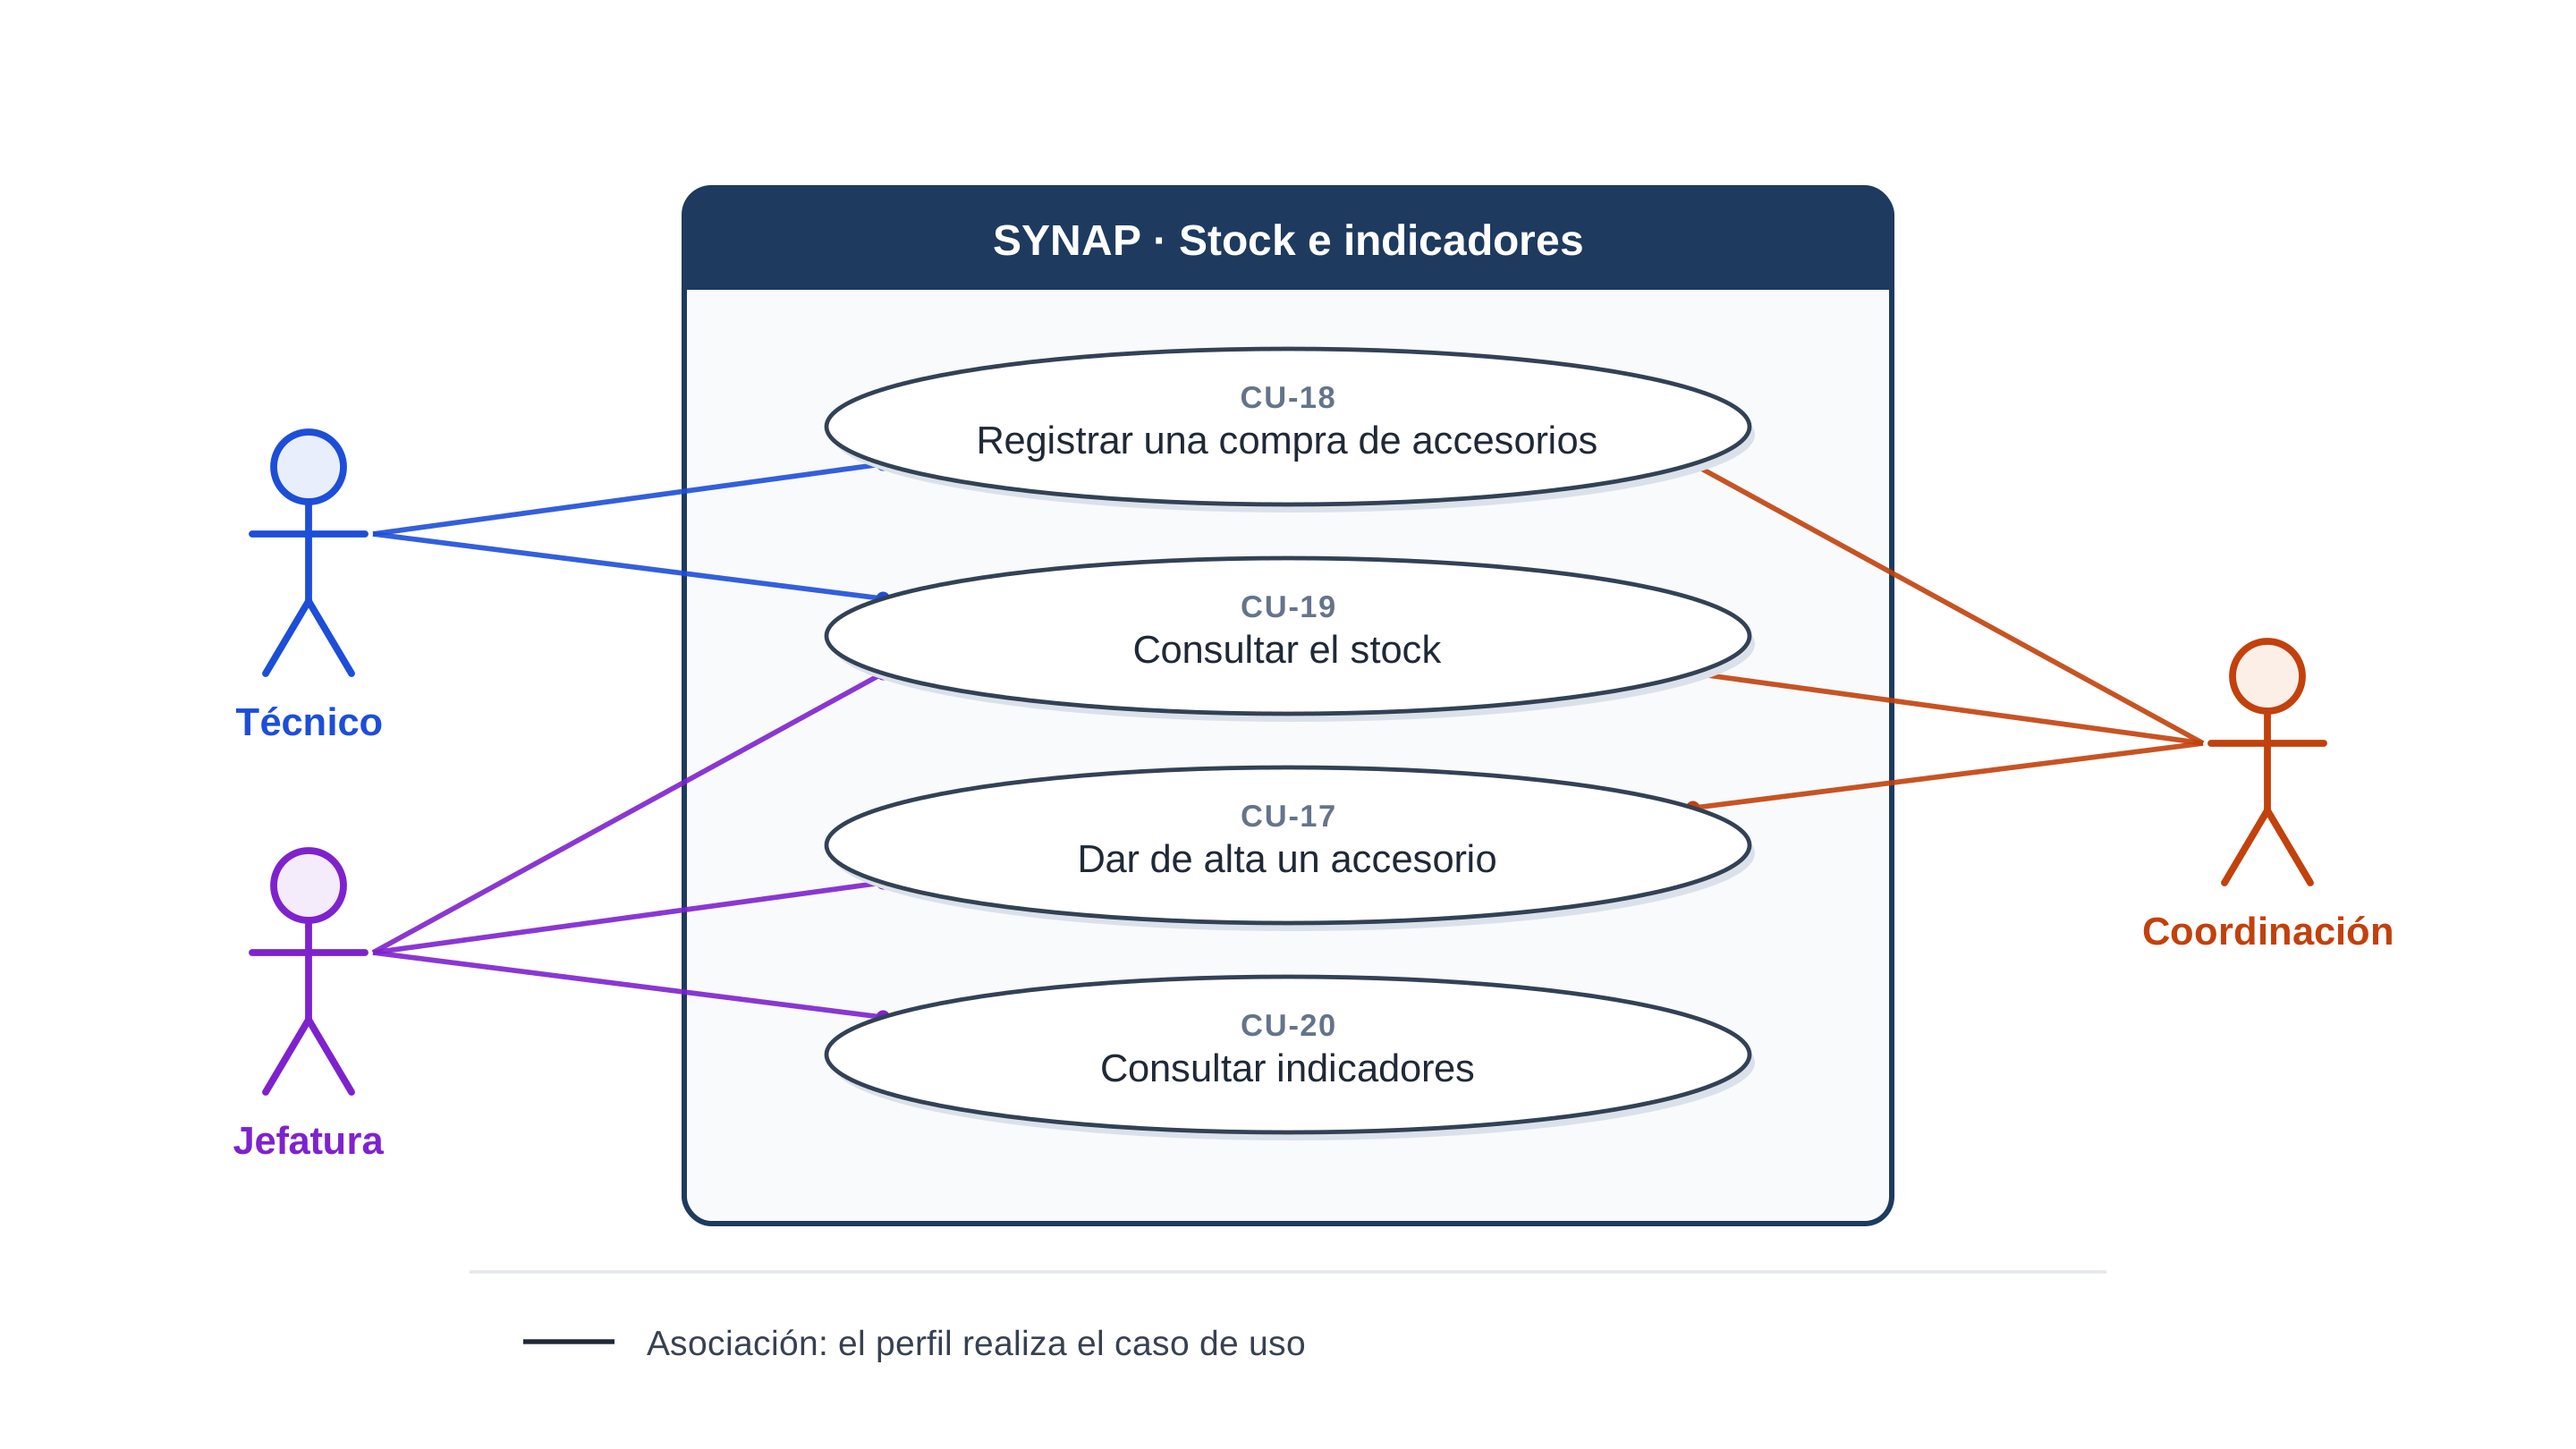
\includegraphics[width=0.9\linewidth]{fotos/Figura_4_4_casos_de_uso_stock_e_indicadores.png}
    \caption{Diagrama de casos de uso del módulo de stock e indicadores.}
    \label{fig:caso-3}
\end{figure}

Los casos de uso con una descripción detallada se presentan en el \ref{anexo:casos-uso}, en la Tabla~\ref{tab:casos-uso}.

\subsubsection{Requerimientos funcionales}
\label{sec:requerimientos-funcionales}

Los requerimientos funcionales describen lo que el sistema debe hacer. Surgieron del relevamiento de los procesos del servicio (sección~\ref{sec:serv-bioing}), de la encuesta (sección~\ref{sec:encuesta}), del análisis de los datos de Maximo (sección~\ref{sec:analisis-maximo}) y del marco normativo y teórico, y suman 31. Abarcan el inventario y las fichas de los equipos, el reporte de fallas, las órdenes de trabajo, el mantenimiento preventivo, el stock de accesorios y los indicadores, además del control de acceso, las notificaciones y la descarga de datos. Cada uno se detalla en el \ref{anexo:requerimientos}, en la Tabla~\ref{tab:rf}, con su origen y los casos de uso que lo cubren, lo que permite seguir el camino desde la necesidad detectada hasta la funcionalidad construida.

\subsubsection{Requerimientos no funcionales}
\label{sec:requerimientos-no-funcionales}

Los requerimientos no funcionales establecen cómo debe comportarse el sistema, más allá de lo que hace. Se definieron once, que abarcan la accesibilidad, la adaptabilidad, la usabilidad, la legibilidad visual, el rendimiento, la seguridad, la integridad de los datos, la trazabilidad, la consistencia temporal, la mantenibilidad y el costo. Seis surgieron de lo planteado en la encuesta, sobre todo de las dificultades con el sistema actual, como la lentitud, la cantidad de pasos y la falta de indicaciones visuales, uno proviene de la normativa y cuatro de criterios técnicos de diseño. Se detallan en el \ref{anexo:requerimientos}, en la Tabla~\ref{tab:rnf}.

\subsection{Datos de partida y modelo de datos}
El modelo de datos es la base sobre la que se apoya todo el sistema, y cualquier error en esta etapa se arrastra a cada módulo que se construye encima. Por eso, como se mencionó en la sección~\ref{sec:enfoque-trabajo}, no se diseñó desde cero. Se partió de la estructura con la que el Hospital Alemán registra hoy su información, se corrigieron los problemas detectados en el histórico de órdenes y en la base de activos (sección~\ref{sec:analisis-maximo}) y se incorporaron los datos que el servicio necesita empezar a registrar para que los requerimientos definidos puedan cumplirse. 

\subsubsection{Bases existentes}
\label{sec:bases-existentes}
La información del servicio se encuentra hoy repartida en varios soportes. El principal es Maximo, donde se registran el inventario de activos, las solicitudes de servicio, las órdenes de trabajo y los planes de mantenimiento. A esto se suman las planillas internas de cada grupo, en las que se anticipan los preventivos de los meses siguientes, los registros en papel archivados en las carpetas físicas de cada equipo, el relevamiento del parque tecnológico realizado en 2024 y el relevamiento de las 3.081 ubicaciones del hospital, en el que cada una tiene un código jerárquico según edificio, piso y sector. 

Como punto de partida para el modelo se tomó la estructura del inventario de activos de Maximo, analizada en la sección~\ref{sec:analisis-maximo}. De esa estructura se conservaron los datos que el servicio ya utiliza y conoce. El principal es el código de activo, con su formato de cuatro segmentos, que además está impreso en las etiquetas de identificación de los equipos. También se conservaron la ubicación, codificada según edificio, piso y sector, el servicio, la marca, el modelo, el número de serie, el grupo de trabajo, la fecha de instalación y el estado. Mantener esa estructura tiene una ventaja práctica: el personal no necesita aprender una nueva forma de identificar los equipos, y la migración de los datos reales, que se aborda en la sección~\ref{sec:integracion-datos}, se simplifica.

Lo que cambió fue la forma de cargar esos datos. Los campos que en Maximo son texto libre pasaron a elegirse de catálogos cerrados siempre que fue posible. El código pasó a construirse de manera automática. El estado quedó como un campo con valores definidos, sin repetirse dentro de la descripción. Además, dejaron de ser necesarios los registros genéricos que hoy funcionan como falsos activos para canalizar pedidos, ya que el sistema permite registrar una solicitud que no corresponde a un equipo médico sin asociarla a un activo.

A esa base se sumaron los datos que hoy no se registran en ningún lado y que resultan indispensables para calcular los indicadores descritos en la sección~\ref{sec:indicadores-gestion}. Entre ellos están la fecha y hora en que se notifica cada falla, los insumos y repuestos consumidos en cada intervención, la frecuencia de mantenimiento de cada equipo y la justificación de los preventivos realizados fuera de término.


\subsubsection{Modelo de datos de SYNAP}
\label{sec:modelo-datos}
El modelo tiene 28 tablas relacionadas y se organiza alrededor del activo: su código identifica a cada equipo en todo el sistema, y cada solicitud, orden de trabajo, mantenimiento o consumo de accesorios queda asociado a él. Esto responde a la trazabilidad que exige la Ley 26.906 \cite{ley_26906}: cada equipo tiene un identificador único y su historia completa puede recuperarse desde un único registro.

\textbf{Activos y catálogos.} El código mantiene el formato del hospital, pero lo construye el sistema: quien da de alta un equipo indica el área y elige su tipo de un catálogo cerrado, y el sistema asigna el siguiente número correlativo de ese tipo y arma el código completo, de modo que no pueden repetirse ni construirse mal los identificadores. Los tipos de equipo y los servicios también son catálogos, y la descripción de cada equipo se completa con el nombre de su tipo. La ubicación se elige de un catálogo cargado a partir del relevamiento de las 3.081 ubicaciones, del que solo se ofrecen las operativas, y un glosario de 778 siglas asocia cada segmento de los códigos de ubicación con su significado. Ese glosario no se cargó a mano: se derivó comparando la descripción de cada ubicación con la de la que la contiene, por ejemplo “E01-1SS-IMAG” con “E01-1SS”. Para el cálculo del nivel de riesgo (sección~\ref{sec:criticidad-riesgo}) se agregaron dos tablas, con los valores del PRIUX de cada tipo de equipo y los datos de soporte de cada modelo.

\textbf{Grupos y usuarios.} El grupo responsable de cada equipo se deduce de su tipo, a través de una tabla que relaciona los grupos con los tipos de equipo, de modo que reasignar un tipo a otro grupo requiere un único cambio. Cada usuario tiene un perfil y, si es técnico, un grupo, y cada grupo registra a su coordinador, por lo que una misma persona puede coordinar varios.

\textbf{Solicitudes y órdenes de trabajo.} Son entidades separadas: la solicitud es un pedido que todavía puede rechazarse o corregirse, y solo al ser aceptada por coordinación da origen a una orden. Ambas tienen un número correlativo legible, además de su identificador interno. La orden registra su tipo (preventiva o correctiva), su estado, el técnico asignado (que puede quedar vacío hasta que alguien la toma), el tiempo que el equipo estuvo fuera de servicio y una referencia a otra orden, que se completa cuando una correctiva se abre a partir de un preventivo. Cada orden tiene además una bitácora con entradas fechadas y firmadas por su autor.

\textbf{Mantenimiento preventivo.} Los planes definen un checklist por tipo de equipo, o uno genérico para los tipos que no tienen el propio, y todo checklist termina con dos ítems fijos: “Necesidad de correctivo” y “Equipo operativo”. De cada mantenimiento se guarda el resultado de cada ítem (pasa o no pasa) con una observación. Cada activo guarda la frecuencia de su mantenimiento y la fecha del próximo, con las que una tarea programada genera las órdenes de cada mes y reprograma el ciclo siguiente. Cada mantenimiento realizado conserva su fecha de realización y, si corresponde, la justificación del retraso, datos necesarios para calcular el cumplimiento del plan.

\textbf{Stock.} Los accesorios y repuestos se registran con su cantidad y dos umbrales, el stock mínimo y el punto de reposición, que definen los niveles de alerta. Las compras tienen dos etapas, pedido y recepción, y solo la recepción modifica el stock. Los consumos en una intervención se vinculan a su orden de trabajo, lo que permite saber qué se usó en cada una y sobre qué equipo, información que hoy el servicio no registra.

\textbf{Conservación del historial.} Como criterio general, la información no se elimina sino que cambia de estado, de modo que el historial se conserva completo (RNF-08). El modelo incluye además tablas para registrar los movimientos de los equipos entre servicios y los cambios hechos sobre los datos, que todavía no están incorporadas a la aplicación y se plantean como trabajo futuro (capítulo~\ref{sec:futuro}).

\subsubsection{Estados de las solicitudes, órdenes de trabajo y mantenimientos}
\label{sec:estados}

Cada solicitud, orden de trabajo y mantenimiento preventivo tiene un estado que indica en qué etapa se encuentra (Figura~\ref{fig:estados-ots}). Los estados son pocos y no se superponen, a diferencia del histórico de Maximo, donde tres de los nueve valores del campo son formas de dar una orden por finalizada (sección~\ref{sec:analisis-maximo}). Además, cada cambio de estado corresponde a una acción concreta del sistema, sin depender de que alguien lo actualice a mano.

\textbf{Solicitudes.} Toda solicitud nace pendiente. Coordinación la revisa: si la acepta, pasa a aceptada y en ese momento se genera la orden correctiva; si la rechaza, pasa a rechazada y el motivo queda visible para quien la envió. Al aceptarla, coordinación clasifica además la falla como técnica o de usuario, por ejemplo por mal uso del equipo. Solo las técnicas cuentan en los indicadores de falla (inactividad, MTBF y MTTR), mientras que las de usuario quedan registradas y siguen sumando a la carga de trabajo del servicio. Quien envió la solicitud puede ver si su pedido ya fue asignado a un técnico.

\textbf{Órdenes de trabajo.} Toda orden nace abierta, ya sea que surja de una solicitud aceptada, de una correctiva detectada durante un preventivo o de la generación mensual de preventivos, y pasa a en progreso cuando se comienza a trabajar en ella, con registro de quién la inició. Una correctiva la cierra directamente el técnico asignado o el coordinador del grupo. Una preventiva, en cambio, pasa antes por pendiente de cierre: el técnico completa el checklist y coordinación la revisa, y puede autorizar el cierre o devolverla con un motivo, que se agrega a la bitácora y deja la orden otra vez en progreso. Al pasar a cerrada se registran la fecha y quién cerró la orden, y ya no admite nuevas entradas en la bitácora.

\textbf{Mantenimientos preventivos.} Cuando se genera una orden preventiva para un equipo con plan de mantenimiento, se crea un registro que la vincula con su checklist y con el mes programado. Ese registro nace pendiente y pasa a realizado cuando el técnico completa la orden, y no cuando coordinación autoriza el cierre, porque para el plan importa la fecha de ejecución y no la de revisión. En ese momento el sistema compara el mes de realización con el programado: si coinciden, el mantenimiento se considera cumplido en término; si no, se exige una justificación del retraso antes de permitir completar la orden. Si coordinación devuelve la orden, al completarla de nuevo se repite esa comparación con la nueva fecha. Un mantenimiento que sigue pendiente cuando termina el mes se considera vencido: el sistema lo calcula y no lo guarda como un estado aparte. Así queda registrado cuáles se hicieron a tiempo, que es la base del indicador de cumplimiento del plan. 

\begin{figure}[H]
    \centering
    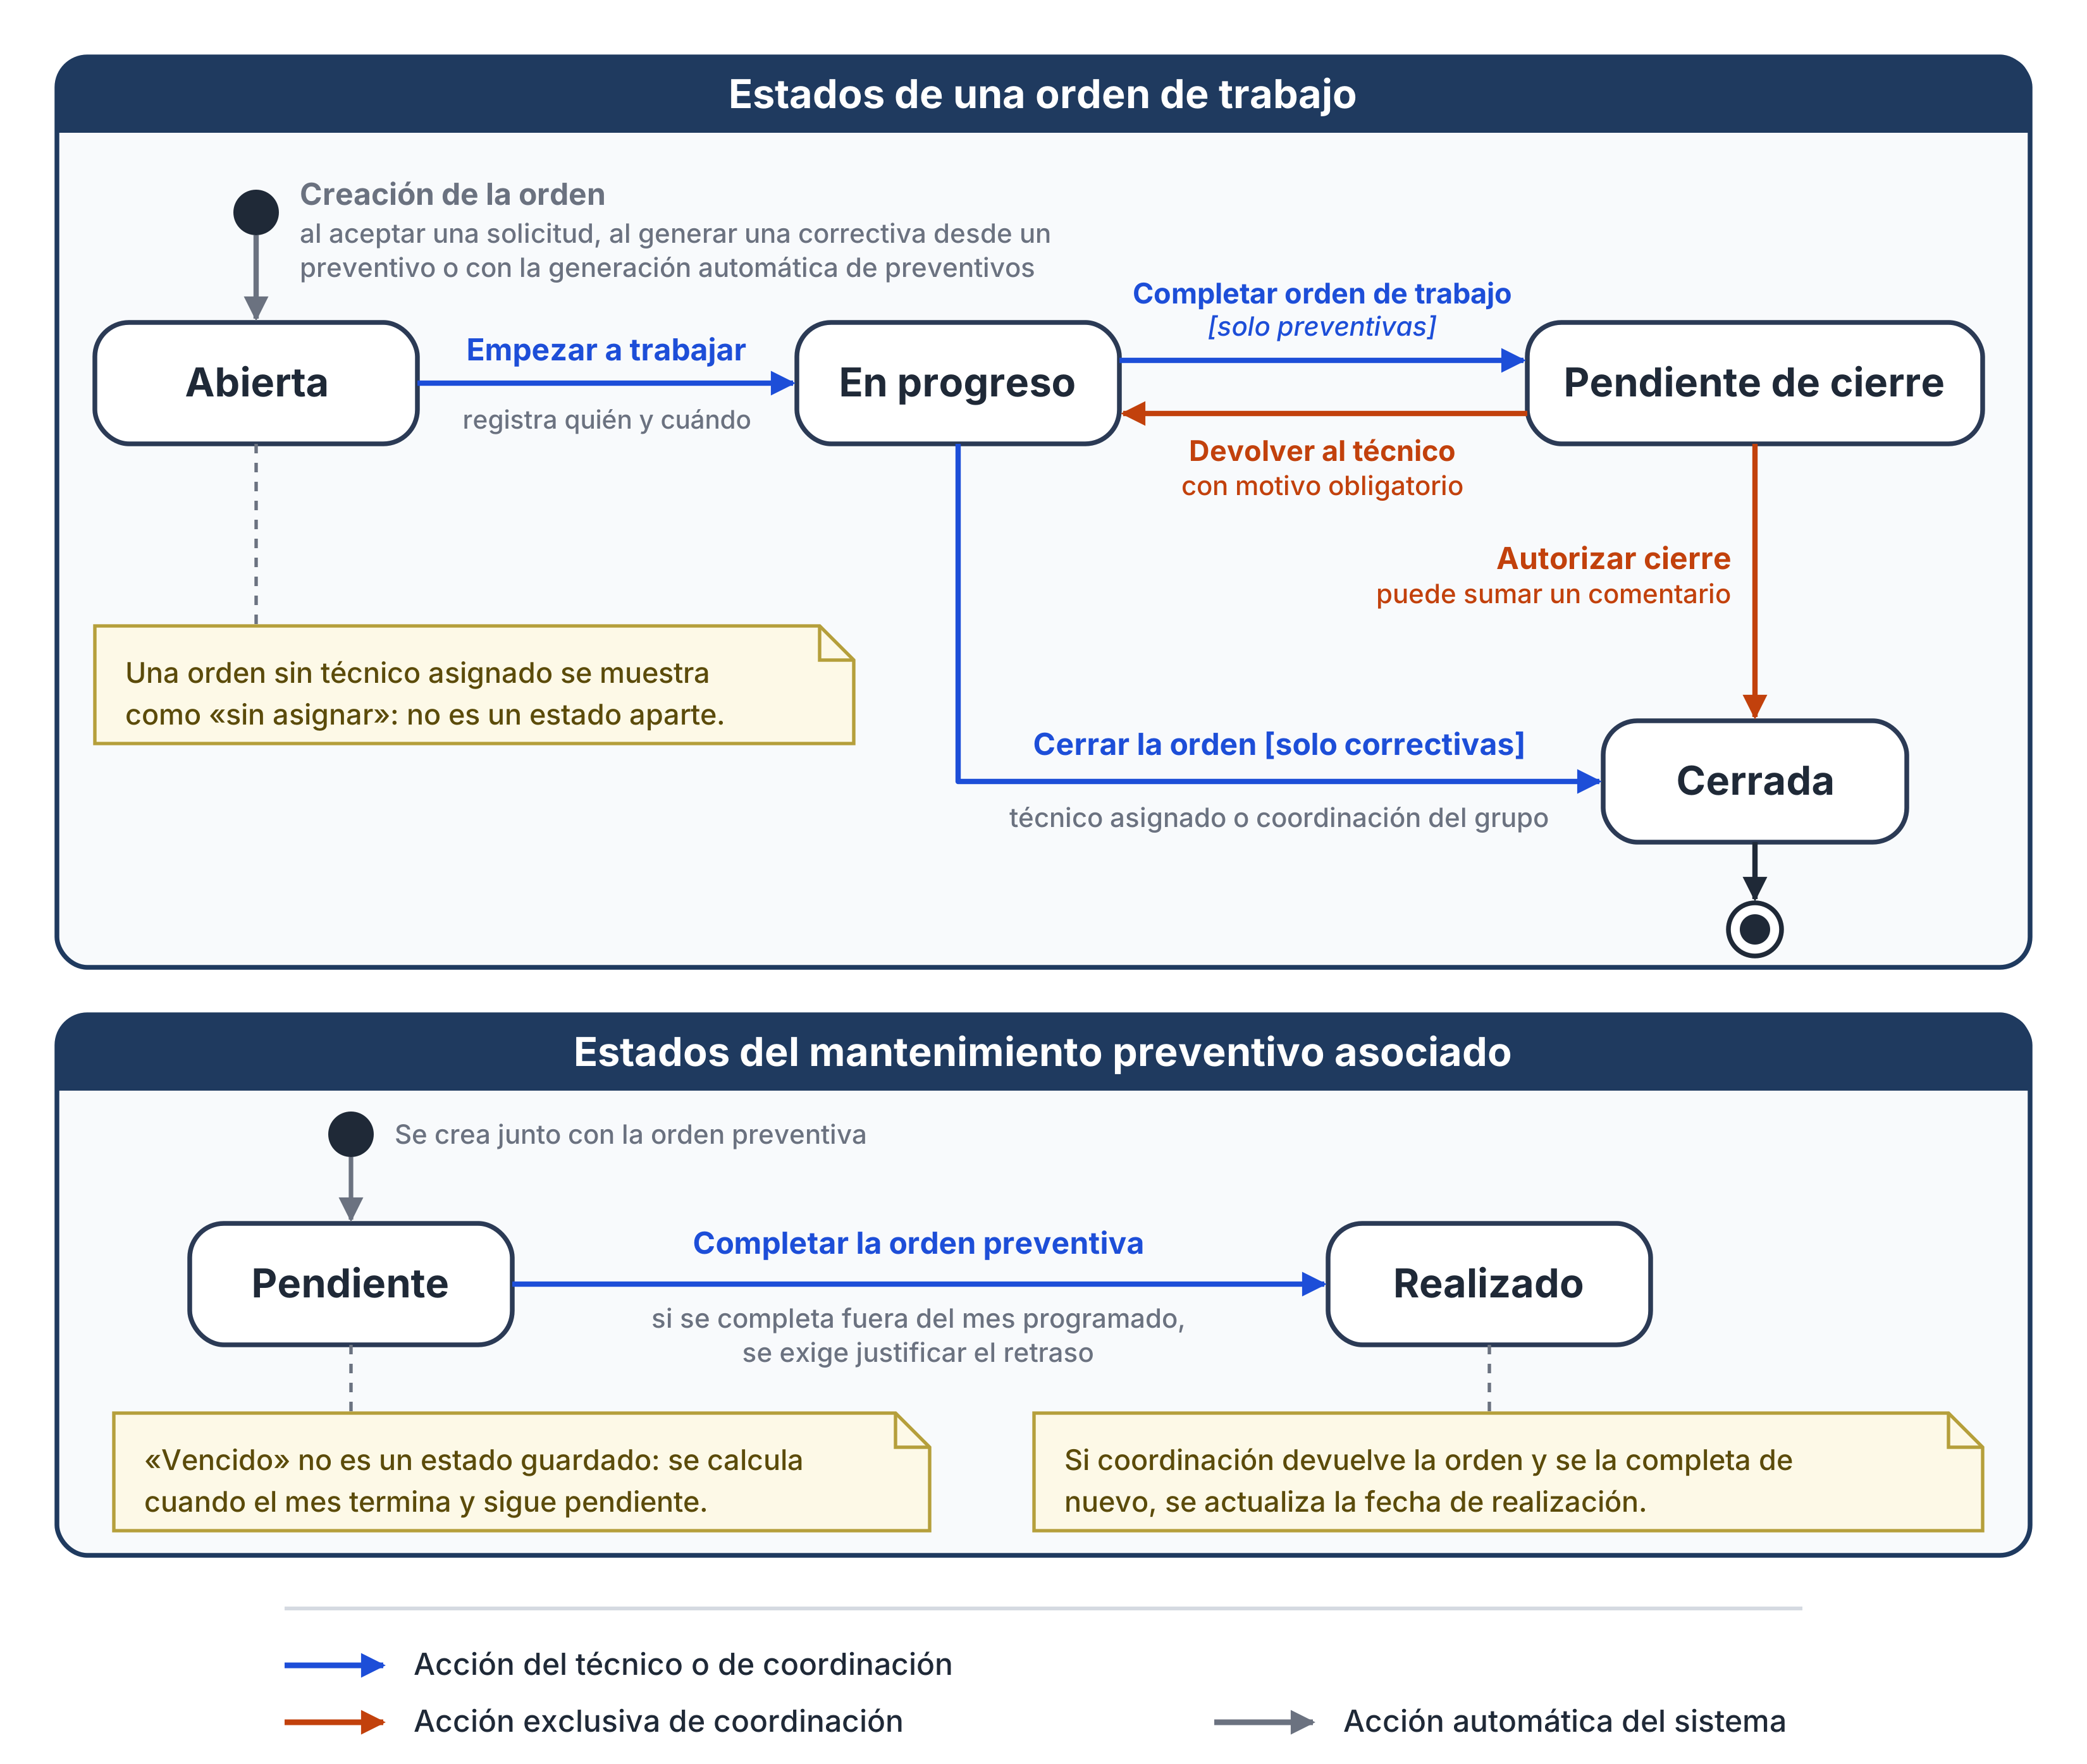
\includegraphics[width=0.9\linewidth]{fotos/Figura_4_6_estados_OT_y_MP.png}
    \caption{Estados de una orden de trabajo y de un mantenimiento preventivo.}
    \label{fig:estados-ots}
\end{figure}

\subsubsection{Datos de prueba}
\label{sec:datos-prueba}
Durante el desarrollo y las pruebas funcionales se trabajó con una base de datos ficticia, construida con la misma estructura y los mismos formatos que las bases del hospital. Se replicaron los formatos de código de activo y de ubicación, los tipos de equipo, los servicios y los grupos, y se crearon usuarios de prueba para cada uno de los cuatro perfiles, ya que los nombres, correos y documentos del personal son información confidencial. Esto permitió probar cada módulo en condiciones realistas sin exponer información confidencial de la institución. Los datos reales del hospital se incorporaron después, en una base separada, como se describe en la sección~\ref{sec:integracion-datos}.

\subsubsection{Criticidad y nivel de riesgo de los equipos}
\label{sec:criticidad-riesgo}

Como se planteó en la sección~\ref{sec:plan-mantenimiento}, el Hospital Alemán clasifica sus equipos con las tablas de riesgo PRIUX, que siguen la lógica del modelo de Fennigkoh y Smith \cite{fennigkoh_smith}. Hasta ahora ese cálculo se hacía por fuera del sistema de gestión, y SYNAP lo realiza de forma automática para cada equipo médico.

El puntaje de riesgo ($R$) se calcula según la Ecuación~\eqref{eq:riesgo} y combina tres variables: la criticidad, que es la suma de la función del equipo y del riesgo de su aplicación clínica, ambos valorados de 1 a 5; el tipo de mantenimiento, que refleja la complejidad del que requiere el equipo; y la antigüedad, de 1 a 5 según los años transcurridos desde su instalación.

\begin{equation}
R = \alpha_0 \cdot \text{Criticidad} + \alpha_1 \cdot \text{Tipo de mantenimiento} + \alpha_2 \cdot \text{Antigüedad}
\label{eq:riesgo}
\end{equation}

En la Ecuación~\eqref{eq:riesgo}, los pesos ($\alpha$) parten de 1 y aumentan cuando se da alguna situación que agrava las consecuencias de una falla: que el equipo no tenga reemplazo, que haya superado su vida útil, que no cuente con soporte de repuestos o de mano de obra, que no tenga proveedor local o que se haya dejado de fabricar. Así, dos equipos con la misma criticidad pueden tener niveles de riesgo muy distintos. El puntaje va de 4 a 75 y se traduce en un nivel alto, medio o bajo.

Como no todos estos datos dependen de lo mismo, cada uno se registra una sola vez, en el nivel que le corresponde. La función, el riesgo clínico, el tipo de mantenimiento y el límite de vida útil son propios del tipo de equipo, de modo que todas las bombas de infusión del hospital comparten esos valores. El soporte, el proveedor local y la continuidad de fabricación dependen de la marca y el modelo; si un modelo no está cargado, se asume que tiene soporte y proveedor y que se sigue fabricando. La disponibilidad de reemplazo es propia de cada equipo, y la antigüedad se calcula desde su fecha de instalación. Así, para evaluar todos los equipos alcanza con completar los valores de cada tipo y de cada modelo, lo que facilita la migración de los datos del hospital.

El puntaje no se almacena: el sistema lo calcula cada vez que se consulta un equipo, por lo que aumenta solo a medida que envejece. Se aplica únicamente a los equipos que el hospital identifica como médicos, y cuando falta la fecha de instalación se muestra la criticidad pero no el puntaje. El nivel de riesgo se muestra en la ficha del equipo y, al aceptar una solicitud, el sistema sugiere la prioridad de la orden correctiva según ese nivel (alta, media o baja), que coordinación puede modificar.

Al implementar las tablas se ajustó el sentido de las preguntas sobre soporte, proveedor y fabricación, de modo que sea la falta de soporte, de proveedor local o de fabricación la que aumenta el riesgo del equipo. Además, como el documento no define a partir de qué puntaje el riesgo es alto, medio o bajo, se adoptaron de manera provisoria los cortes que el hospital usa internamente para sus suministros críticos, 50 y 25 sobre 100, llevados en proporción al puntaje máximo de 75 (37,5 y 18,75). Por ahora el límite de vida útil es el mismo para todos los tipos, 10 años, a la espera de los valores de cada fabricante. Ambos parámetros quedan sujetos a validación con el servicio.

Aparte del cálculo de riesgo, el sistema clasifica cada equipo según su vida útil, con el criterio del hospital, que depende solo de la antigüedad: moderno (menos de 5 años), aceptable (de 5 a menos de 10), medianamente aceptable (de 10 a menos de 15) y obsoleto (15 años o más). Esta clasificación se aplica a cualquier equipo que tenga fecha de instalación, sea médico o no, y se muestra en su ficha y en el panel de indicadores. Es independiente del límite de vida útil del cálculo de riesgo: la clasificación describe el estado general del parque, mientras que el límite agrava el puntaje de cada equipo que lo supera.

\subsection{Arquitectura y tecnologías}
\label{sec:arquitectura-tecnologias}
SYNAP es una aplicación web: se usa desde el navegador y no requiere instalar nada en las computadoras ni en los celulares del hospital. La decisión responde a que el sistema debe estar disponible tanto para un técnico frente a su escritorio como para una enfermera que encuentra un equipo con problemas en medio de un turno, y pedirle que instale una aplicación sería una barrera más entre la falla y su registro. Las tecnologías se eligieron con tres criterios: que fueran de uso libre y sin costos de licencia, que contaran con documentación y comunidad amplias para resolver problemas durante el desarrollo, y que resultaran razonables de mantener por alguien que retome el proyecto en el futuro. 

\subsubsection{Arquitectura general}
El sistema se divide en tres capas (Figura~\ref{fig:arq}). El frontend es la interfaz que corre en el navegador, donde el personal carga y consulta los datos de equipos, órdenes y mantenimientos. Por otro lado, el backend es el servidor de la aplicación que se encarga de recibir los pedidos, aplicar las reglas del sistema y decidir qué se puede hacer y qué no. La base de datos guarda toda la información de forma permanente.

La comunicación sigue siempre el mismo recorrido: el navegador envía un pedido al backend; este verifica quién lo hace y si tiene permiso, consulta o modifica la base y devuelve una respuesta que el navegador muestra. El navegador nunca se comunica directamente con la base, y esto es intencional: cualquiera puede inspeccionar lo que ocurre dentro de su navegador, por lo que las credenciales de la base quedarían expuestas si estuvieran ahí. Además, como las reglas del sistema viven solo en el backend, el comportamiento sería el mismo desde otra interfaz, como una aplicación nativa.

\begin{figure}[H]
    \centering
    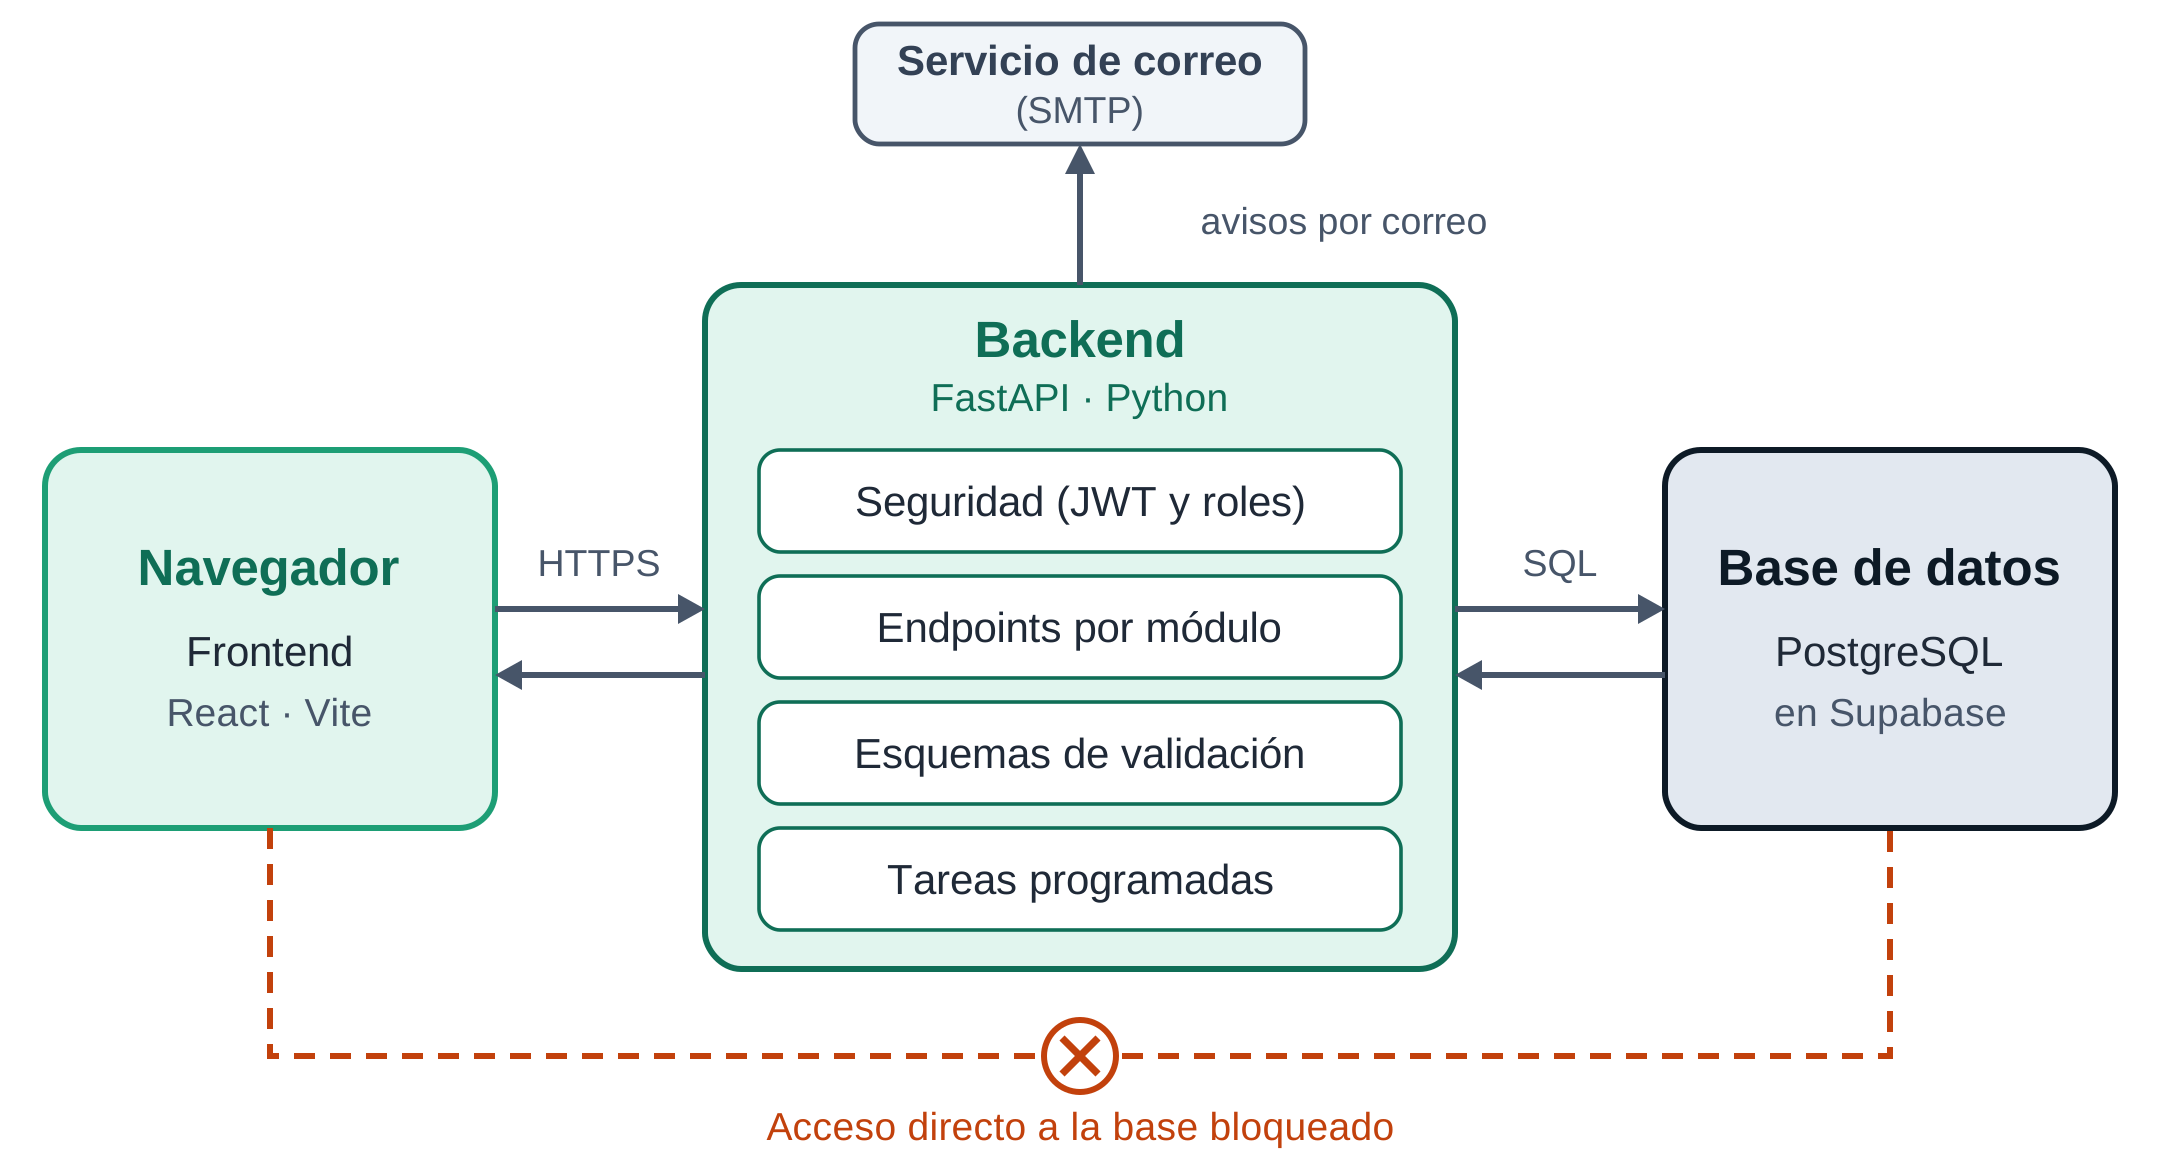
\includegraphics[width=0.9\linewidth]{fotos/Figura_4_7_arquitectura.png}
    \caption{Arquitectura de SYNAP. El navegador se comunica solo con el backend, que accede a la base de datos y envía los avisos por correo.}
    \label{fig:arq}
\end{figure}

\subsubsection{Backend y base de datos}
\label{sec:backend-bd}

El backend se encuentra implementado en Python (v3.11.4), un lenguaje ampliamente utilizado en el desarrollo de aplicaciones web, con documentación abundante y una comunidad grande detrás. Sobre él se construyó una interfaz de programación de aplicaciones (API, por sus siglas en inglés), que es el conjunto de direcciones a las que el frontend le pide o le envía información, por ejemplo una para consultar los datos de un activo y otra para registrar una falla. Cada una de esas direcciones se denomina endpoint.

Para construir la API se utilizó FastAPI (v0.141.1), una herramienta que provee la estructura base sobre la que se escriben los endpoints, evitando tener que programar desde cero el manejo de las conexiones. Se escogió ya que valida automáticamente que los datos que llegan tengan la forma esperada, de manera que información incompleta o mal cargada nunca alcanza la base, y además, genera por su cuenta una documentación interactiva de todos los endpoints disponibles, que durante el desarrollo permitió probar cada funcionalidad desde el navegador antes de que existiera una sola pantalla. 

Cada endpoint se identifica por su dirección y por el tipo de operación que realiza, lo que en el Protocolo de Transferencia de Hipertexto (HTTP, por sus siglas en inglés) se conoce como método. Se utilizaron en el sistema las siguientes operaciones:
\begin{itemize}
    \item GET: se utiliza para consultar información de la base sin modificar nada, como cuando se abre la ficha de un activo o se lista el stock de insumos. 
    \item POST: se utiliza para crear algo que antes no existía, por ejemplo al reportar una falla o al registrar el consumo de un repuesto. 
    \item PATCH: se utiliza para modificar de forma parcial un registro ya creado, como al cambiar el estado de una orden de trabajo sin tocar el resto de sus datos. 
    \item DELETE: se utiliza para eliminar un registro, aunque en este sistema prácticamente no se usa, ya que la información no se borra sino que cambia de estado, de manera que el historial se conserva.
\end{itemize}

Al separar las operaciones por método, una misma dirección puede responder de manera distinta según lo que se le pida, y el sistema puede definir qué perfiles tienen permitido consultar cierta información y cuáles además pueden modificarla, como se puede observar en la Figura~\ref{fig:endpoints}.

\begin{figure}[H]
    \centering
    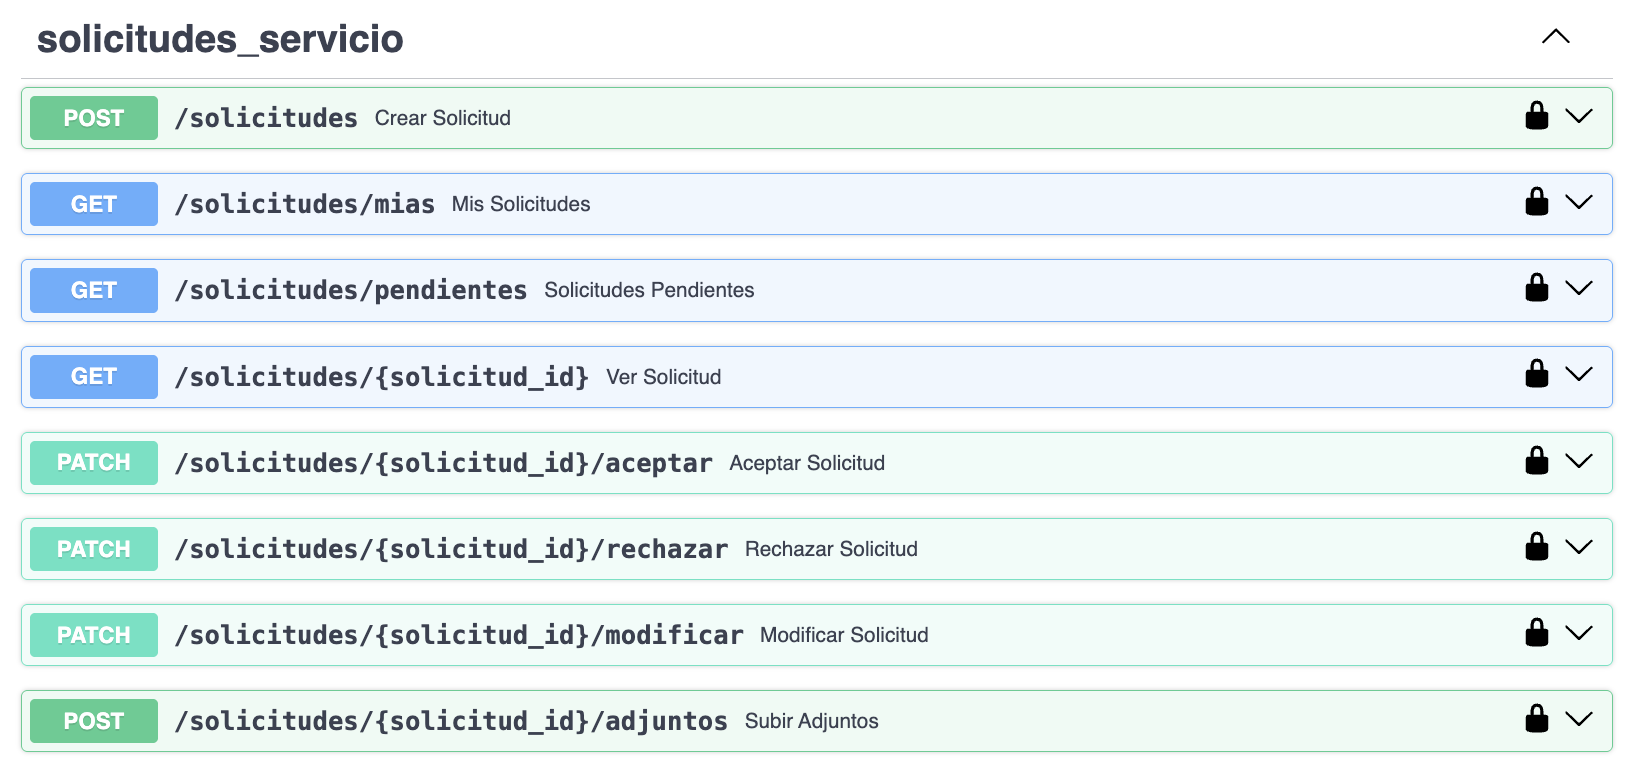
\includegraphics[width=1\linewidth]{fotos/endpoints}
    \caption[Endpoints del módulo de solicitudes de servicio en la documentación de FastAPI.]{Endpoints del módulo de solicitudes de servicio en la documentación interactiva generada por FastAPI. Se observa cómo una misma dirección responde a distintos métodos según la operación solicitada.}
    \label{fig:endpoints}
\end{figure}

El código está organizado por temas y no en un único archivo. Cada área del sistema tiene su propio módulo de rutas, de modo que todo lo relacionado con activos vive en un lugar y lo de órdenes de trabajo en otro, tal como se detalla en la Tabla~\ref{tab:backend}. Los archivos restantes concentran las funciones transversales, es decir, la conexión con la base, la definición de las tablas, los contratos de entrada y salida, la seguridad, el cálculo de riesgo, los informes, los correos y las tareas programadas.

\begin{table}[H]
    \caption{Módulos de rutas del backend.}
    \label{tab:backend}
    \centering
    \begin{tabular}{>{\raggedright\arraybackslash}p{4.2cm} >{\raggedright\arraybackslash}p{\dimexpr\linewidth-4.2cm-2\tabcolsep\relax}}
        \toprule
        \textbf{Módulo} & \textbf{Responsabilidad} \\
        \midrule
        \texttt{auth} & Activación de cuenta, inicio de sesión y recuperación de contraseña \\
        \texttt{usuarios} & Consulta de usuarios del sistema \\
        \texttt{activos} & Ficha de cada equipo, búsqueda y acceso mediante código QR \\
        \texttt{solicitudes} & Reporte de fallas por parte de enfermería, con sus archivos adjuntos \\
        \texttt{ordenes\_trabajo} & Apertura, asignación, seguimiento y cierre de órdenes \\
        \texttt{preventivas} & Generación de las órdenes de mantenimiento preventivo del período \\
        \texttt{mantenimientos} & Consulta del historial de mantenimientos de cada equipo \\
        \texttt{planes\_mantenimiento} & Definición de los planes por tipo de equipo \\
        \texttt{checklists} & Plantillas de verificación y registro de sus resultados \\
        \texttt{stock} & Insumos, compras, consumos y alertas de reposición \\
        \texttt{dashboard} & Cálculo de los indicadores de gestión \\
        \texttt{exportar} & Descarga de la información en formato CSV \\
        \texttt{catalogos} & Glosario de siglas y catálogo de ubicaciones validadas del hospital \\
        \bottomrule
    \end{tabular}
\end{table}
Cada endpoint define además qué información acepta y qué información devuelve, a través de estructuras llamadas esquemas. Su función es doble. Por un lado validan la entrada, de modo que si falta un campo obligatorio o llega con un tipo equivocado, el pedido se rechaza antes de tocar la base. Por el otro acotan la salida, lo que significa que solo se devuelve aquello que fue declarado explícitamente, y por eso datos como el hash de una contraseña nunca salen del backend aunque estén guardados en la misma tabla que el resto de la información del usuario.

Para comunicarse con la base se usó SQLAlchemy (v2.0.52), que permite trabajar con las tablas como objetos de Python en lugar de escribir consultas SQL a mano, lo que hace el código más legible y evita una familia de vulnerabilidades que aparecen cuando las consultas se arman concatenando texto. Todas las tablas se reflejan en un único archivo, que replica la estructura creada en Supabase. El motor es PostgreSQL, relacional y de código abierto, adecuado porque cada elemento del sistema depende de otro: una orden de trabajo existe porque hay un activo al que corresponde, y un consumo de accesorios porque hay una orden en la que se usó. Esas dependencias se declaran como restricciones, de modo que el motor mismo impide, por ejemplo, registrar una orden para un equipo inexistente.

La base está alojada en Supabase, que la ofrece como servicio en la nube y evitó instalar y mantener un servidor. Se aprovecha solo el alojamiento: la autenticación se resolvió dentro del backend. Como Supabase ofrece además una vía propia de acceso a los datos que no pasa por el backend, se la bloqueó de manera deliberada activando la seguridad a nivel de fila en las tablas, de modo que la única entrada a la información es FastAPI, donde cada pedido se valida según quién lo hace y qué rol tiene.

Cada pedido abre su propia sesión con la base y la cierra al terminar, pase lo que pase. Las operaciones que deben ocurrir juntas se confirman de una sola vez: por ejemplo, el consumo de un accesorio y el descuento del stock, de modo que no puede quedar un consumo asentado sin que el stock baje ni al revés. Como el servicio cierra las conexiones inactivas, el sistema verifica que la conexión siga viva antes de reutilizarla y la renueva cada 30 minutos, lo que evita errores intermitentes.

En cuanto a la seguridad del software, las contraseñas no se guardan tal como el usuario las escribe. Antes de llegar a la base pasan por bcrypt (v4.0.1), una función que las transforma en una cadena de caracteres irreconocible y que funciona en un solo sentido, de manera que nadie puede recuperar la contraseña original a partir de lo que quedó guardado. Para verificar un ingreso, el sistema le aplica la misma transformación a lo que el usuario escribió y compara si coinciden.

Una vez que el usuario ingresa al sistema, este necesita reconocerlo en cada pantalla que abre sin volver a pedirle la contraseña, y para eso se utiliza un token web JSON (JWT, por sus siglas en inglés). Se trata de una credencial temporal que el backend entrega al iniciar sesión y que el navegador adjunta en cada pedido posterior, y que identifica al usuario por su número. Para impedir que ese contenido se altere, el backend le agrega una firma calculada a partir de la información del token y de una clave secreta que solo el servidor conoce, y la verifica en cada pedido. El rol, en cambio, no viaja en el token sino que se consulta en la base cada vez, de modo que no hay forma de asignarse otro editando la credencial, y un cambio de rol se aplica en el pedido siguiente sin esperar a que el token venza.

Verificada la validez del token, el sistema pasa a controlar qué puede hacer esa persona. Cada endpoint declara qué perfiles tienen permitido utilizarlo, y esa verificación está escrita en una única función reutilizable que se ejecuta antes que el resto y corta el pedido si el rol no alcanza, de manera que el control no depende de que se recuerde escribirlo endpoint por endpoint. La función tiene dos variantes según el tipo de operación, ya que en la general jefatura siempre pasa porque necesita visión completa del servicio, mientras que en la estricta queda afuera, y esta última se aplica a las acciones operativas como cerrar una orden, que jefatura supervisa pero no ejecuta. Gracias a esta distinción, jefatura puede consultar las órdenes de trabajo de todos los grupos, pero el backend rechaza cualquier intento de modificarlas. 

Cuando un pedido no puede completarse, el sistema responde indicando el motivo en lugar de fallar sin explicación, y para eso utiliza los códigos previstos por el protocolo HTTP. Un token vencido o inválido devuelve 401, un rol insuficiente 403, un recurso inexistente 404, un dato con formato inválido 422 y una acción que no cumple las reglas del sistema 400, lo que permite que el frontend muestre un mensaje comprensible en cada caso.

Por otro lado, las solicitudes admiten archivos adjuntos, como fotografías del equipo, que se guardan en la propia base junto con su nombre y tipo, con un límite de 5 archivos de 4 MB por solicitud. La alternativa habitual es un servicio de archivos separado, pero para pocos archivos de tamaño acotado habría implicado credenciales adicionales y un punto más de falla sin beneficio real. Por último, las fechas con hora se guardan en horario universal y el frontend las muestra en la hora local, para que un cambio de huso horario no altere el orden de dos eventos consecutivos. 

Además, el backend incorpora tres herramientas para las tareas que no responden a un pedido directo del usuario en pantalla: el envío de correos, la generación de informes y la ejecución de tareas programadas.

\textbf{Envío de correos.} El sistema envía correos por SMTP a través de Brevo, un servicio de envío con plan gratuito. Las credenciales y la dirección del remitente, que debe estar verificada en Brevo, se leen de variables de entorno y no forman parte del código; lo mismo ocurre con la dirección de la aplicación con la que se arman los enlaces de los correos, que se configura según el entorno en el que se publica el sistema (sección~\ref{sec:despliegue}). Los mensajes son de dos tipos: el enlace para restablecer la contraseña, que llega al correo personal del usuario, vence a la hora y puede usarse una sola vez, y los avisos automáticos del sistema (orden correctiva creada, stock crítico y mantenimiento próximo a vencer), que llegan siempre a una única casilla del servicio. Si no hay credenciales cargadas, el mensaje se muestra en la consola del backend en lugar de enviarse, lo que permite probar el resto del sistema sin configurar nada. Si el envío falla, el error queda registrado pero no interrumpe la operación, de modo que una orden o un ajuste de stock se guardan aunque el aviso no salga. 

\textbf{Generación de informes en PDF.} Los informes se generan con ReportLab (v5.0.1), en memoria y cada vez que se solicitan, con los datos vigentes en ese momento; no se guardan como archivos. Hay dos tipos de informes que se pueden descargar: el informe de cada mantenimiento preventivo cerrado, que reúne los datos del equipo y de la orden y el resultado de cada punto del checklist (sección~\ref{sec:mantenimiento-preventivo}), y el informe de un equipo, con sus datos y el historial completo de sus órdenes de trabajo (sección~\ref{sec:activos-qr}).

\textbf{Tareas programadas.} Se ejecutan con APScheduler (v3.11.3), dentro del propio proceso del backend y con la hora de Buenos Aires, por lo que no requieren un servicio aparte. Al iniciarse el backend y todos los días a las 00:05 se generan las órdenes preventivas del mes en curso; a las 00:10 se verifica si ya comenzó la última semana del mes y, de ser así, se avisa de los mantenimientos del mes que todavía no se realizaron. Cada aviso se marca en el mantenimiento correspondiente para no repetirse los días siguientes, y la generación de órdenes está diseñada para poder ejecutarse más de una vez sin duplicar las ya existentes. Gracias a ello, la ejecución al iniciar el backend recupera el caso en que haya estado apagado el primer día del mes. Si una tarea falla, el error se registra y se reintenta en la siguiente ejecución, sin detener el backend. En la versión publicada, estas tareas se disparan de otra forma, descrita en la sección~\ref{sec:despliegue}, y su funcionamiento desde el punto de vista del usuario se describe en las secciones~\ref{sec:mantenimiento-preventivo} y~\ref{sec:notificaciones}.


\subsubsection{Frontend}

La interfaz se construyó con React (v19.2.8), una biblioteca de JavaScript que organiza la pantalla en componentes, es decir, piezas independientes que se escriben una vez y se reutilizan. Así, elementos como el encabezado que acompaña cada pantalla se definen en un solo archivo, se ven y se comportan igual en toda la aplicación y cualquier cambio se aplica una sola vez. Como entorno de desarrollo se utilizó Vite (v8.2.2), que levanta un servidor local y aplica cada cambio guardado de inmediato, sin recargar la página ni perder el estado de la pantalla que se está modificando. 

El proyecto está organizado en cuatro grupos de archivos que cumplen funciones distintas: 
\begin{itemize}
    \item Páginas - pages. Corresponden a cada pantalla completa del sistema, desde el inicio de sesión hasta el panel de indicadores. 
    \item Componentes - componentes. Reúnen las piezas que aparecen en más de una pantalla, como el armazón general que envuelve a todas o el checklist de un mantenimiento preventivo. 
    \item Comunicación con el backend - api. Concentra todas las llamadas al servidor, con un archivo por tema que agrupa las relacionadas con activos, órdenes, stock y demás.
    \item Utilidades - utiles. Reúnen funciones auxiliares, como el formato de fechas y el tratamiento de los códigos.
\end{itemize}
La capa api se diseñó para que las pantallas no se comuniquen directamente con el backend. Cuando una necesita información se la pide a la función correspondiente, que es la única que conoce la dirección y el formato del pedido. Si algo cambia en el backend, se corrige en ese archivo y no en cada pantalla que lo usaba. 

El token y el rol del usuario se guardan en el almacenamiento local del navegador, por lo que la sesión se mantiene aunque la persona cierre la pestaña, hasta que el token vence (un día) o ella cierra sesión. Si un pedido es rechazado porque el token venció, la aplicación borra la sesión guardada y vuelve al inicio de sesión. Esto resulta razonable en un servicio donde se entra y se sale del sistema varias veces por turno. Existen alternativas más resistentes a ciertos tipos de ataque, pero se consideró adecuada esta opción para un prototipo de uso interno. 

La navegación entre pantallas se resuelve con react-router-dom (v7.18.2), que asigna una dirección propia a cada vista y permite moverse entre ellas sin recargar la página completa. A partir del rol guardado en la sesión, la aplicación determina qué opciones se muestran en cada caso, de manera que la interfaz acompaña el control de accesos que el backend aplica por detrás. 

El escaneo de códigos QR se resuelve con html5-qrcode (v2.3.8), una biblioteca que accede a la cámara del dispositivo desde el propio navegador, lo que evitó desarrollar una aplicación nativa solo para esa función. La contrapartida es que los navegadores habilitan la cámara únicamente sobre conexiones seguras, por lo que durante el desarrollo fue necesario probarlo a través de un túnel HTTPS, y la versión publicada se sirve bajo ese mismo protocolo (sección~\ref{sec:despliegue}). 

Por último, los gráficos de la aplicación, como los del panel de indicadores, se generan con recharts (v3.10.1), y el aspecto visual se apoya en un archivo central de estilos que define colores, tipografía y estilos reutilizables, cuyos criterios se desarrollan en la sección~\ref{sec:interfaz-perfil}.

\subsubsection{Interfaz}
\label{sec:interfaz-perfil}
SYNAP se pensó desde el principio para usarse tanto en una computadora como en un celular, ya que no todos los perfiles trabajan en el mismo lugar. Un técnico suele consultar órdenes y cargar datos desde su escritorio, mientras que una enfermera que encuentra un equipo con una falla necesita poder reportarla en el momento, escaneando su código QR con el teléfono (sección~\ref{sec:activos-qr}). Por eso la interfaz es responsive, es decir, se adapta al ancho de la pantalla en la que se abre. En una computadora, la navegación entre pestañas se ubica en una barra lateral, y cuando la pantalla es angosta, como la de un celular, esa barra se reemplaza por un encabezado arriba y un menú de pestañas abajo, al alcance del pulgar, como en cualquier aplicación móvil. El contenido se reacomoda para ocupar el ancho disponible, de manera que la misma pantalla se puede usar en ambos dispositivos sin perder información (Figura~\ref{fig:responsive}).

\begin{figure}[H]
    \centering
    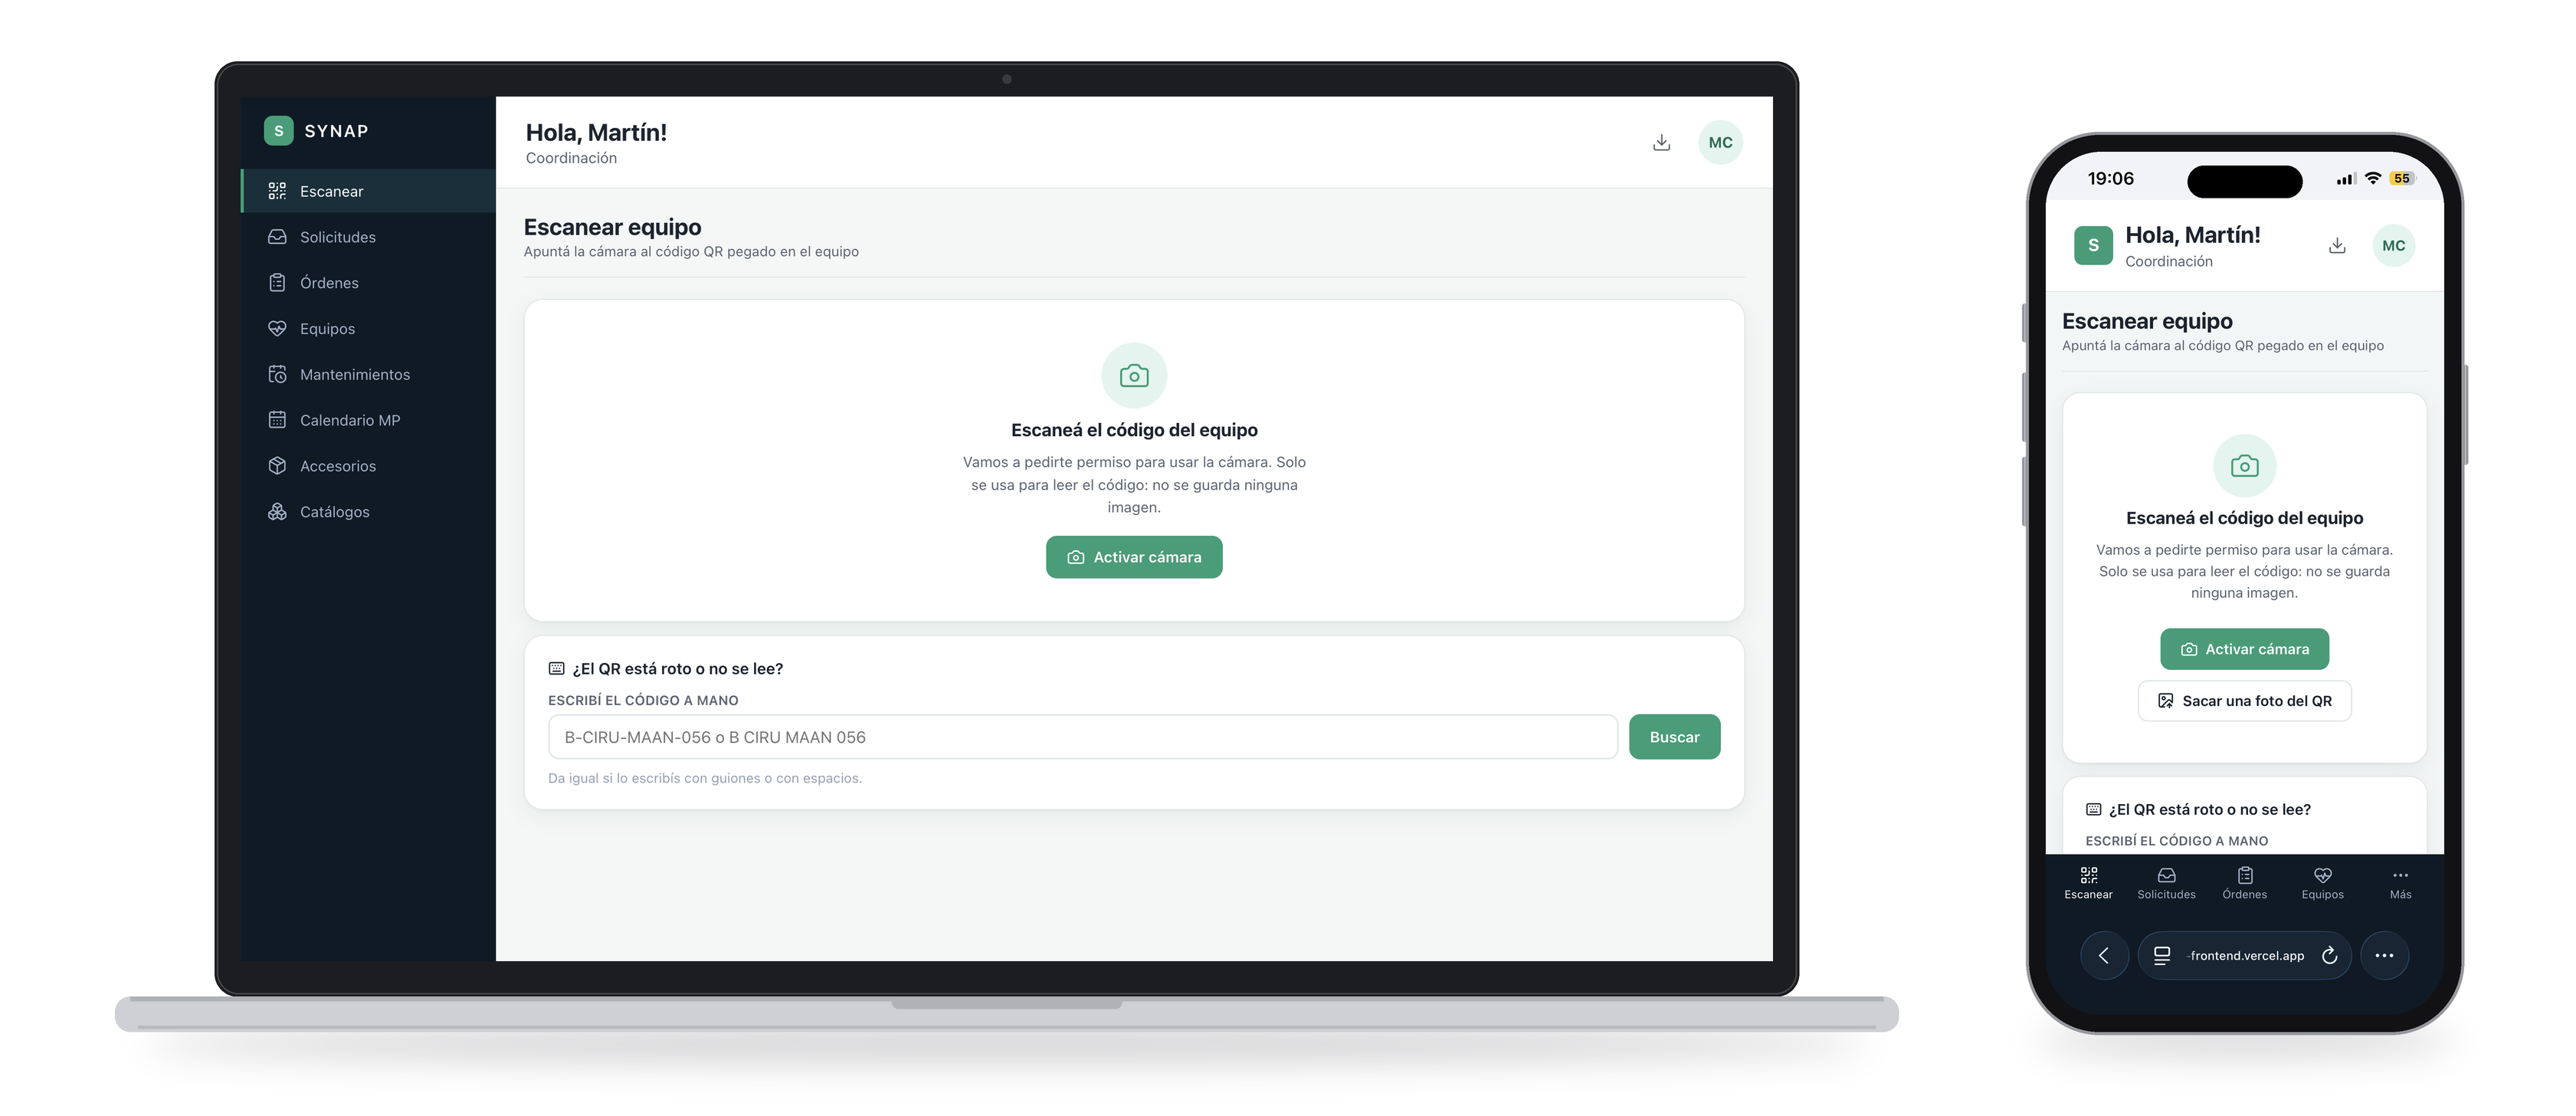
\includegraphics[width=\linewidth,height=0.42\textheight,keepaspectratio]{fotos/synap_computadora_vs_celular.png}
    \caption{Pantalla de escaneo de SYNAP en computadora (izquierda) y en celular (derecha).}
    \label{fig:responsive}
\end{figure}

\subsubsection{Despliegue}
\label{sec:despliegue}
Para que SYNAP pudiera usarse fuera de las computadoras de desarrollo, tanto desde una PC del hospital como desde el celular de un técnico, la aplicación se publicó en Vercel, una plataforma de alojamiento web. El frontend y el backend se desplegaron como dos proyectos independientes a partir del mismo repositorio de GitHub, disponible en \url{https://github.com/isteverlynck/synap}, mientras que la base de datos se mantuvo en Supabase. Cada vez que se incorpora un cambio al repositorio, Vercel vuelve a publicar ambos proyectos automáticamente, de modo que la versión disponible siempre coincide con la última del código. La aplicación puede accederse desde cualquier navegador en \url{https://synap-frontend.vercel.app}, con conexión segura (HTTPS), que además es la condición que exigen los navegadores para habilitar la cámara con la que se escanean los códigos QR.

A diferencia de un servidor tradicional, Vercel no mantiene el backend encendido de forma permanente, sino que lo activa con cada pedido. Por eso, las tareas automáticas que en el entorno de desarrollo corren dentro del propio backend (sección~\ref{sec:backend-bd}), como la generación de las órdenes preventivas del mes y el aviso de mantenimientos próximos a vencer, pasaron a dispararse mediante una tarea programada de la plataforma que se ejecuta una vez por día.

\subsection{Desarrollo de los módulos}
\label{sec:desarrollo-modulos}
En esta sección se describe cada módulo del sistema. El orden acompaña el recorrido de la información dentro del servicio, desde el ingreso al sistema y la consulta de un equipo hasta el reporte de una falla, su resolución en una orden de trabajo, el mantenimiento preventivo, el consumo de accesorios y los indicadores de gestión. De cada módulo se explica qué problema resuelve, qué reglas lo gobiernan y cómo quedó implementado en la interfaz.

Como complemento, el \ref{anexo:manual} reúne un manual de uso con los pasos de las tareas más frecuentes de cada perfil, desde el primer ingreso al sistema hasta el reporte de una falla, la resolución de una orden y la consulta de los indicadores.

\subsubsection{Autenticación y control de accesos}
Para ingresar, la persona completa en la pantalla de inicio de sesión (Figura~\ref{fig:inicio-sesion}) su número de identificación y su contraseña. El número tiene la forma u + DNI (por ejemplo, u12345678) y se eligió como nombre de usuario porque es el que el Hospital Alemán ya utiliza para identificar a su personal.

Como las cuentas se cargan sin contraseña, la primera vez que alguien usa el sistema debe activar su usuario desde el botón “¿Primera vez? Activar mi usuario”. La activación tiene dos pasos. Primero se ingresa el número de identificación y el sistema verifica que exista y que todavía no haya sido activado; si no es así, le indica a la persona cómo continuar. Después se elige la contraseña, escribiéndola dos veces para evitar errores de tipeo, con un mínimo de 8 caracteres y sin otras restricciones. De este modo no hace falta distribuir contraseñas iniciales entre el personal, algo poco práctico y menos seguro, y cada persona elige la suya en su primer acceso. 

En el inicio de sesión, si el número no está registrado, la cuenta todavía no fue activada o la contraseña es incorrecta, se muestra el mismo mensaje, “Número o contraseña incorrectos”, y no se permite el acceso. 

\begin{figure}[!htbp]
    \centering
    \newlength{\altofig}\setlength{\altofig}{0.37\linewidth}
    \begin{minipage}[t]{0.30\linewidth}
        \centering
        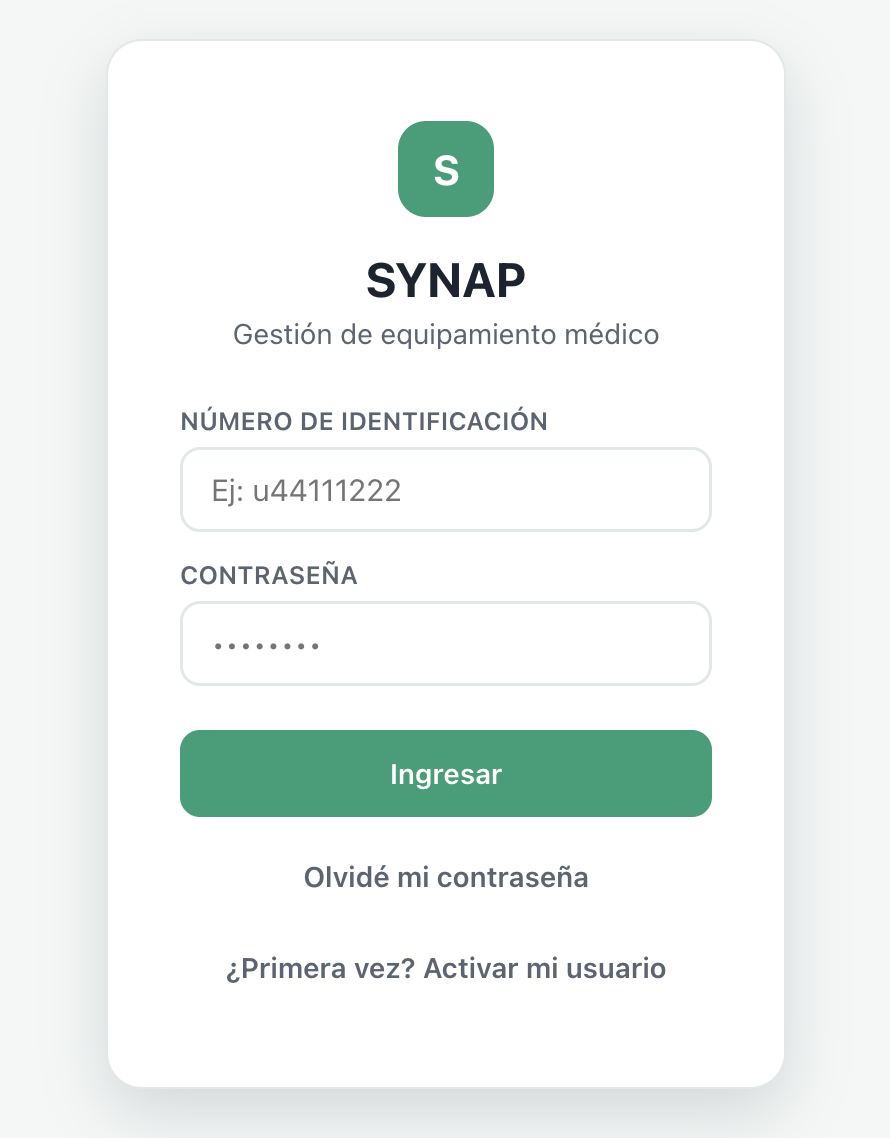
\includegraphics[height=\altofig]{fotos/Figura_4_9a_iniciar_sesion.png}
        \caption{Pantalla de inicio de sesión.}
        \label{fig:inicio-sesion}
    \end{minipage}
    \hfill
    \begin{minipage}[t]{0.66\linewidth}
        \centering
        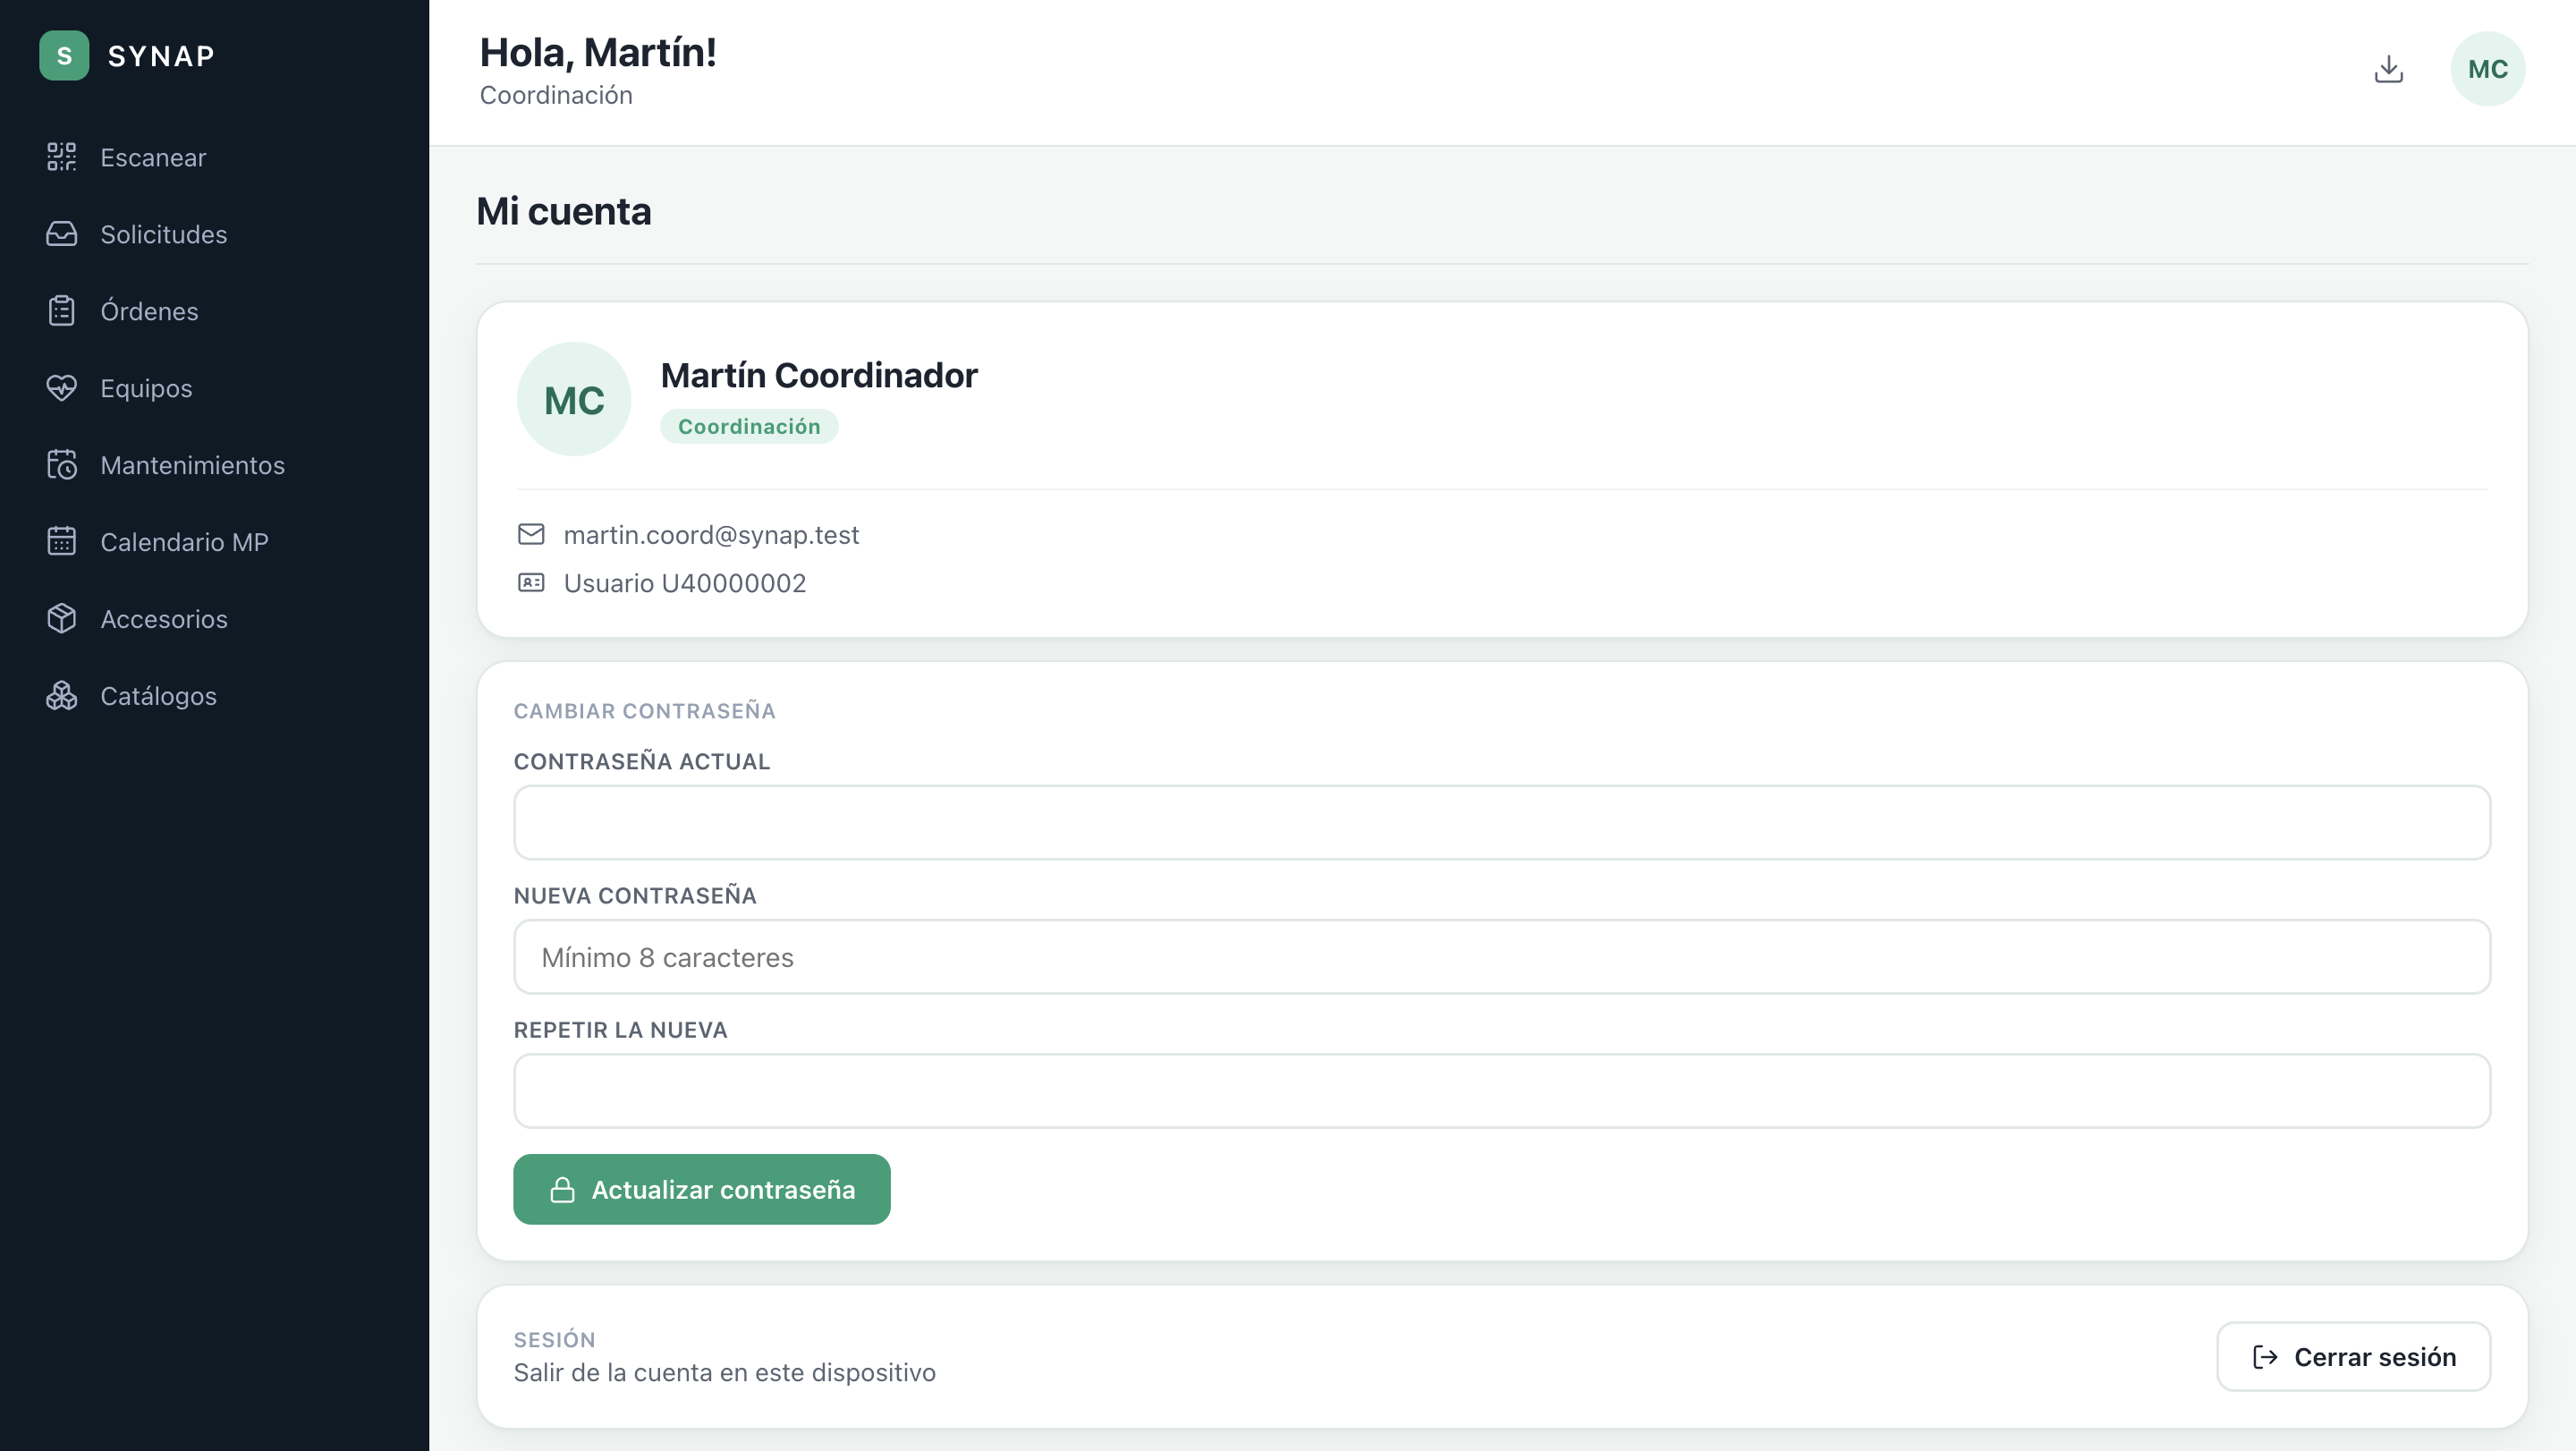
\includegraphics[height=\altofig]{fotos/Figura_4_9b_mi_cuenta.png}
        \caption{Pestaña “Mi cuenta” del perfil de coordinación.}
        \label{fig:mi-cuenta}
    \end{minipage}
\end{figure}

En el caso de que el usuario olvide su contraseña, puede recuperarla desde la misma página de inicio de sesión seleccionando el botón “Olvidé mi contraseña”. Si en cambio desea cambiarla, puede hacerlo desde la pestaña “Mi cuenta” (Figura~\ref{fig:mi-cuenta}), a la que se accede en cualquier momento, una vez iniciada la sesión, desde el ícono ubicado en el extremo superior derecho, identificado con las iniciales de su nombre.

\subsubsection{Activos y acceso por QR}
\label{sec:activos-qr}
El hospital ya tiene colocada en cada equipo una etiqueta con un código QR, un código de barras y el código de activo (sección~\ref{sec:serv-bioing}). Como el QR hoy no cumple ninguna función, el sistema lo aprovecha: contiene únicamente el código del equipo, con el que la aplicación recupera su información. Así no hizo falta generar ni imprimir etiquetas nuevas, una tarea costosa sobre un parque de varios miles de equipos, y el sistema se incorpora sin modificar lo que el servicio ya tiene instalado.

La pestaña “Escanear” abre la cámara del dispositivo y está disponible para todos los perfiles (Figura~\ref{fig:responsive}). Antes de continuar, el sistema verifica que el equipo exista, por si la etiqueta es antigua o el código está mal. Enfermería llega al formulario de solicitud de servicio con el código ya completado, y técnico, coordinación y jefatura, a la ficha del equipo. Si la cámara no funciona o la etiqueta es ilegible, el código puede ingresarse a mano en la misma pantalla, de modo que ninguna de esas situaciones deje al usuario sin acceso a la información.

La pestaña “Equipos”, disponible para todos los perfiles excepto enfermería, lista los equipos de a 50 por página, con su código, ubicación, descripción, marca, modelo y estado (Figura~\ref{fig:equipos}). Permite buscar por código, nombre, marca o número de serie, filtrar por estado, grupo técnico, servicio y tipo de equipo, y registrar un equipo nuevo (técnico, coordinación y jefatura). Al pasar el mouse sobre un código de equipo o de ubicación, un cartel muestra su significado a partir del glosario de siglas y de los catálogos del hospital (por ejemplo, “DESF” se lee como desfibrilador), de modo que los códigos pueden interpretarse sin conocer de memoria todas las siglas.

\begin{figure}[H]
    \centering
    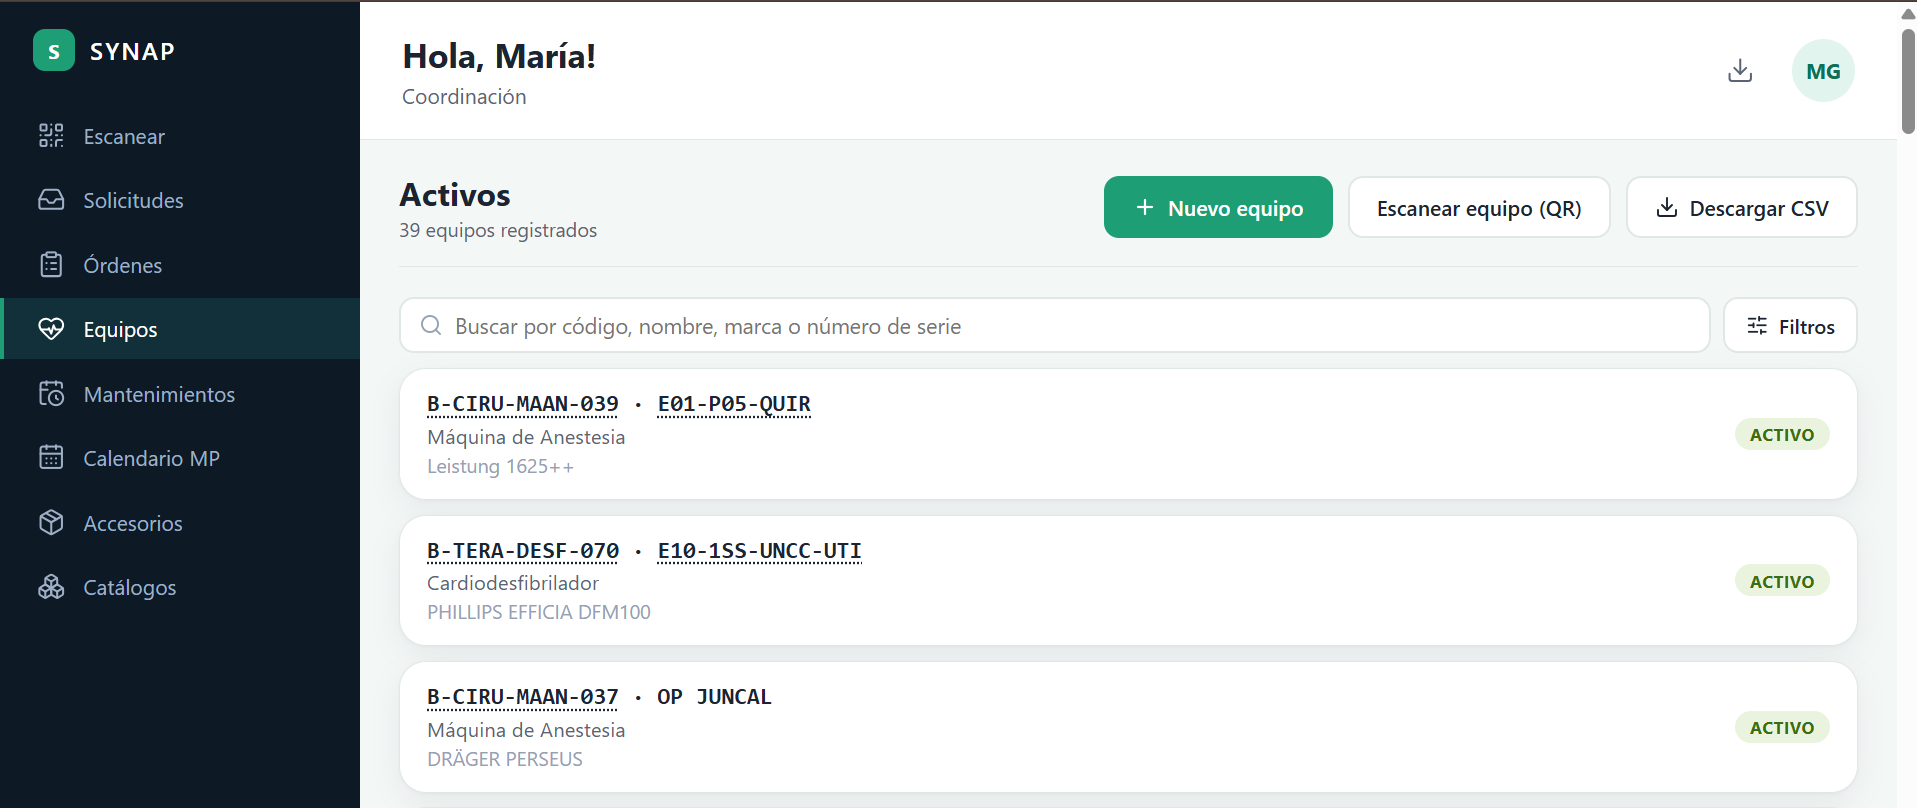
\includegraphics[width=\linewidth,height=0.45\textheight,keepaspectratio]{fotos/Figura_4_11_equipos_coordinacion.png}
    \caption{Pestaña “Equipos” de coordinación.}
    \label{fig:equipos}
\end{figure}

El botón “Nuevo equipo” abre un formulario con campos completables, cuyos datos permiten identificar, ubicar y evaluar el equipo, en línea con la sección~\ref{sec:inventario}. Son obligatorios el área, que se escribe a mano, y el tipo de equipo y el servicio, que se eligen de listas cerradas. La ubicación es opcional pero, si se carga, debe elegirse del catálogo de ubicaciones validadas del hospital. También se registran la marca, el modelo, el número de serie, la orden de compra, la fecha de instalación, el estado y, si ya tiene la etiqueta, el código QR. La casilla “Es equipo médico” indica si se le calcula la criticidad y, solo cuando está marcada, aparece “No tiene backup”, que señala que no hay otro equipo que pueda reemplazarlo y aumenta su nivel de riesgo. Opcionalmente puede programarse su mantenimiento preventivo, indicando en qué mes se abre la primera orden y cada cuántos meses se repite, valor que el sistema sugiere a partir del checklist del tipo de equipo.

El código de activo no se escribe, sino que el sistema lo arma con el formato de las etiquetas (sección~\ref{sec:modelo-datos}), por ejemplo B-INTR-DESF-070. El número correlativo es el siguiente disponible para ese tipo en todo el hospital, sin importar el área, que se carga a mano porque, como se observó en el apartado~\ref{sec:analisis-maximo}, no coincide con el servicio del equipo. A partir del tipo elegido, el sistema completa además la descripción y asigna el grupo técnico responsable. Coordinación y jefatura disponen de la pestaña “Catálogos”, donde dan de alta los tipos de equipo, los servicios y las siglas del glosario.

% \begin{figure}[H]
%     \centering
%     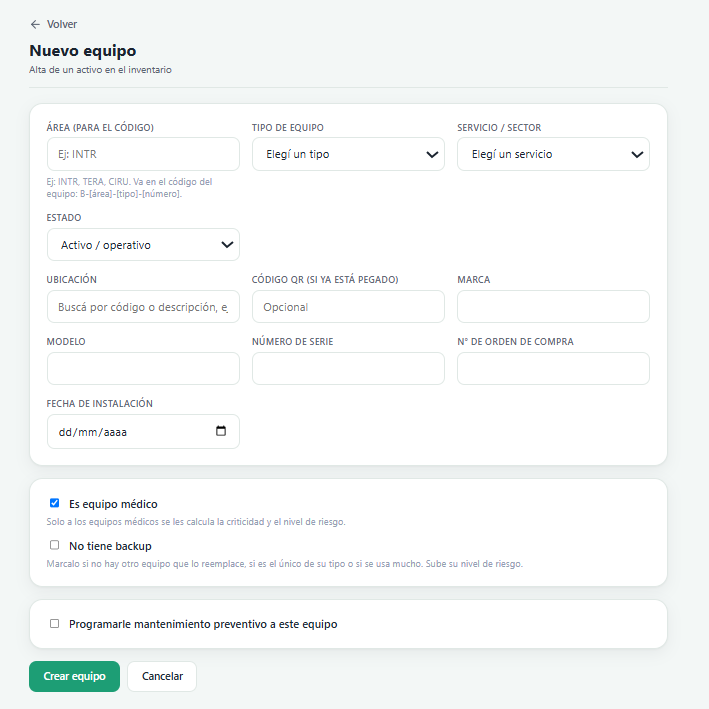
\includegraphics[width=0.62\linewidth,height=0.45\textheight,keepaspectratio]{fotos/Figura_4_12_nuevo_equipo.png}
%     \caption{Formulario “Nuevo equipo” de coordinación.}
%     \label{fig:nuevo-equipo}
% \end{figure}

La ficha de un equipo (Figura~\ref{fig:ficha-equipo}) reúne sus datos, su estado actual, la fecha del próximo mantenimiento preventivo, el grupo de bioingeniería responsable y el historial de órdenes y mantenimientos con su estado. Junto a cada integrante del grupo hay un botón “Contactar” que abre un correo, lo que permite el contacto directo con el bioingeniero a cargo, y el botón “Descargar reporte” genera un PDF con los datos del equipo y el historial completo de sus órdenes. Según el perfil se suman dos accesos: “Ver estado de la reparación”, que lleva a la orden abierta del equipo, si la hay (técnico y coordinación), y “Ver plan de mantenimiento”, que lleva al plan de su tipo (coordinación y jefatura). Técnico y coordinación pueden abrir cada orden del historial dentro de los límites de su grupo; jefatura consulta las órdenes desde la pestaña “Órdenes”, en modo lectura.

Técnico, coordinación y jefatura pueden usar además el botón “Editar ficha”, que abre un formulario con los datos del alta, excepto el área. Antes de guardar, el sistema pide confirmar (“¿Confirmás que querés modificar este equipo?”), porque de la ficha dependen el historial, los indicadores y el nivel de riesgo, y envía solo lo que cambió. No pueden editarse el código, clave con la que se vincula todo el historial, ni las fechas de mantenimiento calculadas por el sistema; si se cambia el tipo de equipo, la descripción y el grupo responsable se recalculan solos. La edición permite corregir errores de carga, actualizar la ubicación cuando un equipo cambia de sector y registrar su baja con el estado “De baja”: el equipo deja de generar preventivos y de figurar en el pronóstico del calendario, pero conserva su historial.

\begin{figure}[H]
    \centering
    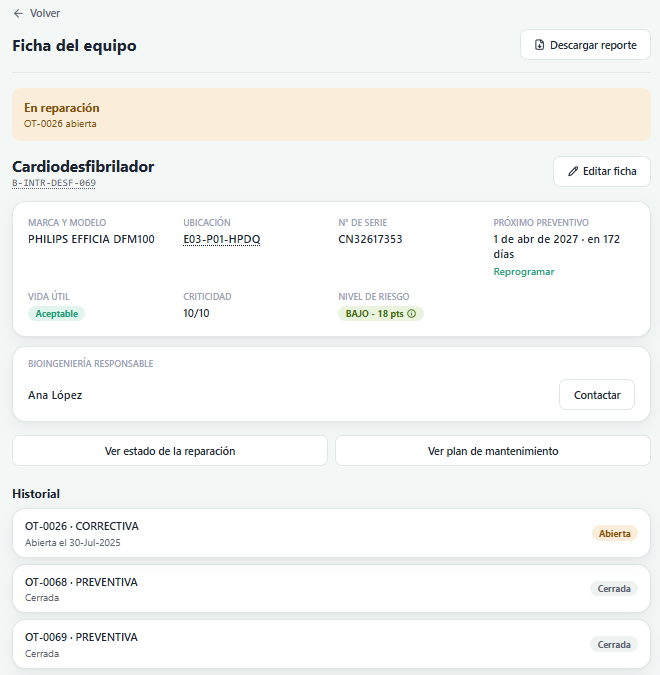
\includegraphics[width=0.55\linewidth,height=0.45\textheight,keepaspectratio]{fotos/Figura_4_13_ficha_equipo.png}
    \caption{Ficha de un equipo, vista de coordinación.}
    \label{fig:ficha-equipo}
\end{figure}

La ficha muestra además el estado de vida útil del equipo y, si es médico, su criticidad y su nivel de riesgo (alto, medio o bajo), calculados como se explicó en la sección~\ref{sec:criticidad-riesgo}; es información de uso interno del servicio y no se muestra a enfermería. Al tocar el nivel de riesgo se abre la ventana “Cómo se calcula” (Figura~\ref{fig:riesgo-calculo}), que ubica el puntaje en una barra con los cortes de cada nivel y detalla los factores y las condiciones que aumentaron su peso. Si falta algún dato, como la fecha de instalación, la ficha indica el motivo en lugar de mostrar un resultado incompleto. El nivel de riesgo también sugiere la prioridad al aceptar una solicitud (sección~\ref{sec:solicitudes}) y se incluye en la descarga de equipos (sección~\ref{sec:descarga-datos}).

\begin{figure}[H]
    \centering
    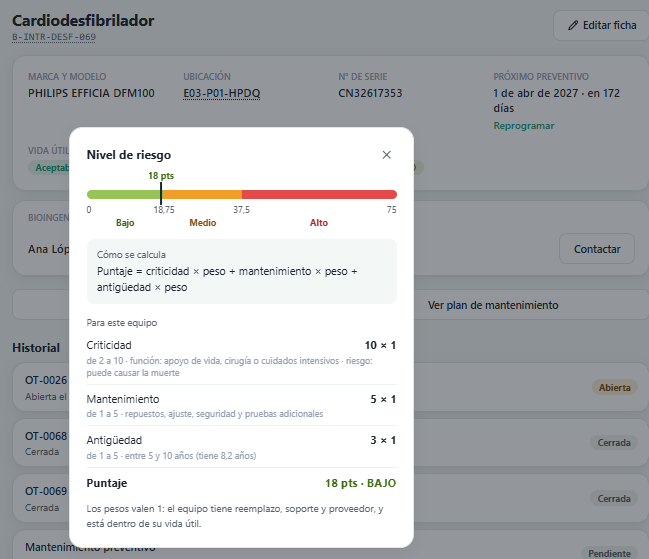
\includegraphics[width=0.55\linewidth,height=0.45\textheight,keepaspectratio]{fotos/Figura_4_14_riesgo_como_se_calcula.png}
    \caption{Ficha con el nivel de riesgo y la ventana “Cómo se calcula”.}
    \label{fig:riesgo-calculo}
\end{figure}

\subsubsection{Reporte y clasificación de fallas (solicitudes de servicio)}
\label{sec:solicitudes}
Cuando un equipo falla, quien lo detecta suele ser quien lo está usando y no Bioingeniería, por lo que el circuito correctivo tiene que empezar ahí. El módulo de solicitudes de servicio es la puerta de entrada de todo trabajo correctivo. La solicitud es una entidad separada de la orden de trabajo porque es un pedido que el servicio debe evaluar antes de comprometer a alguien, y porque así queda registro incluso de los reportes que no derivan en una intervención. Enfermería accede desde la pestaña “Mis solicitudes” y coordinación, desde “Solicitudes”.

\textbf{Enfermería.} Es el único perfil que reporta fallas. En “Mis solicitudes” (Figura~\ref{fig:mis-solicitudes}) se encuentran las opciones “Crear solicitud” (la que se abre por defecto), “Enviadas”, “Aceptadas” y “Rechazadas”, y un botón para escanear el QR de un equipo. El formulario de creación pide:
\begin{itemize}
    \item \textbf{¿Es un equipo médico?} Se responde con “Sí, es un equipo médico” o “No (ej: instrumental)”, porque el servicio también recibe pedidos que no involucran equipamiento registrado y el circuito posterior es distinto en cada caso.
    \item \textbf{Identificador del equipo.} Se valida contra los equipos existentes y sugiere coincidencias mientras se escribe, para que no puedan reportarse equipos inexistentes ni códigos con errores de tipeo; llega completo si el formulario se abrió escaneando el QR. Si no es un equipo médico, se describe en cambio qué es (por ejemplo, una pinza de oftalmología).
    \item \textbf{Descripción de la falla y ubicación.} Ambas son obligatorias. La ubicación se pide porque un equipo puede estar en un lugar distinto del asignado.
    \item \textbf{Fotos o PDF (opcional).} Hasta cinco archivos, con los límites mencionados en la sección~\ref{sec:backend-bd}.
\end{itemize}
Al enviarla, la solicitud recibe un número correlativo. Si es de un equipo médico, se dirige automáticamente al coordinador del grupo técnico que corresponde a su tipo de equipo; si no lo es, la ven todos los coordinadores y quien la toma define el grupo.

\begin{figure}[H]
    \centering
    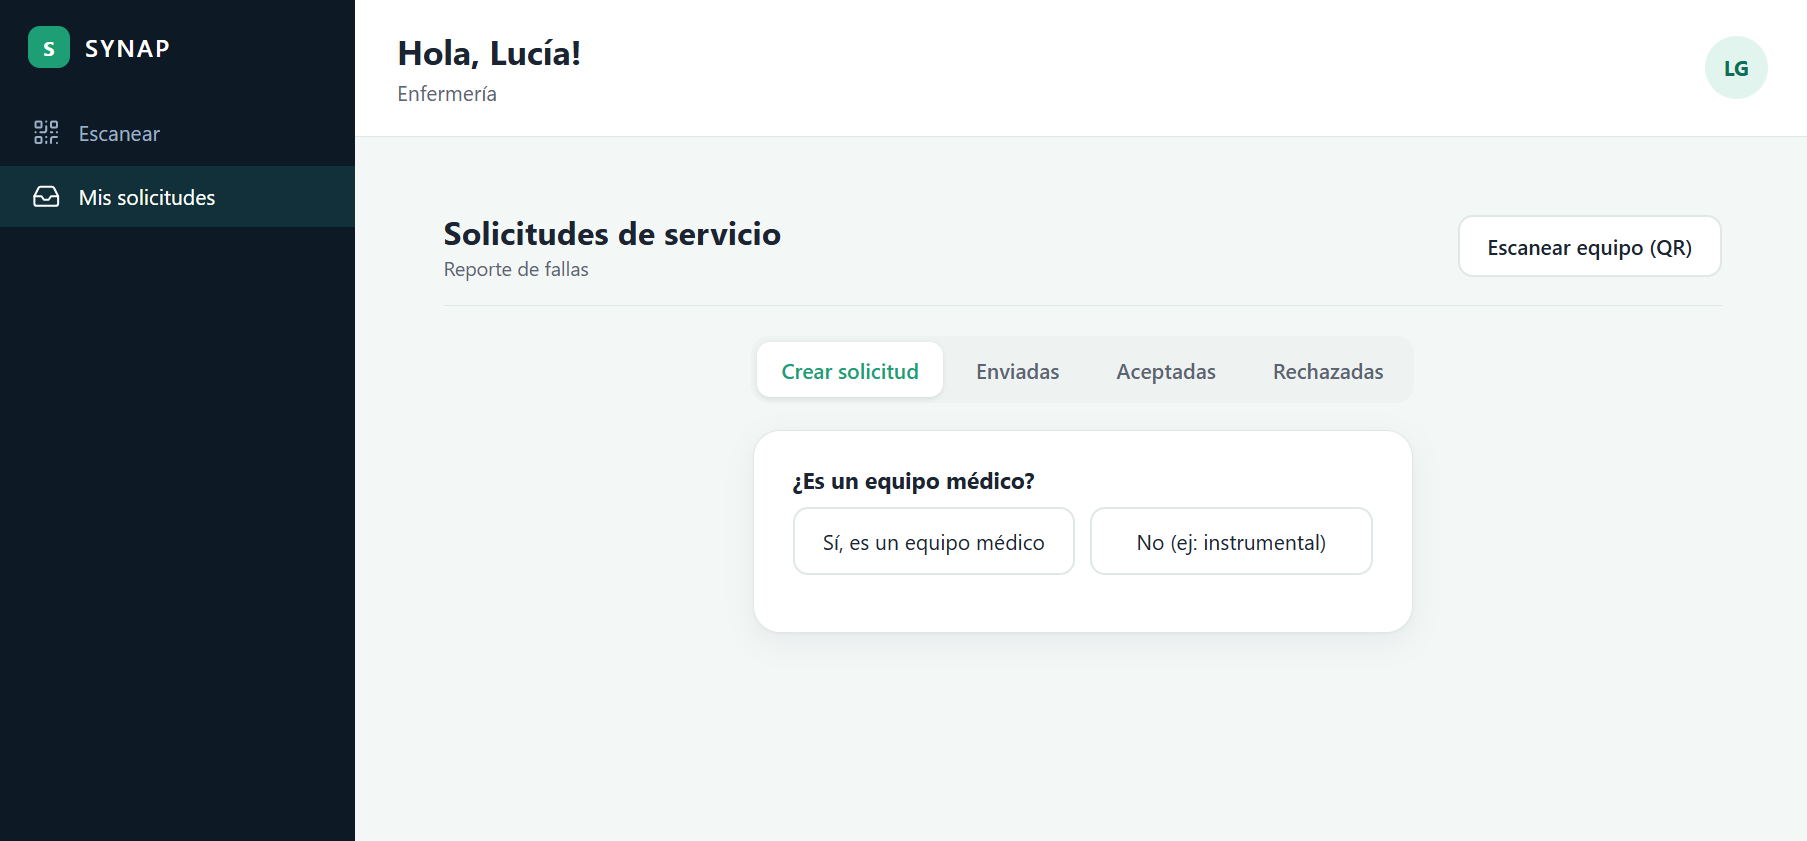
\includegraphics[width=\linewidth,height=0.45\textheight,keepaspectratio]{fotos/Figura_4_15_mis_solicitudes_enfermeria.png}
    \caption{Pestaña “Mis solicitudes” de enfermería, opción “Crear solicitud”.}
    \label{fig:mis-solicitudes}
\end{figure}

Las pestañas “Enviadas”, “Aceptadas” y “Rechazadas” muestran el historial de las solicitudes del propio usuario, con búsqueda por número o por equipo y filtro por fecha. En las aceptadas se indica si el pedido ya tiene un técnico asignado, sin acceso al detalle de la intervención, que excede el interés de enfermería; en las rechazadas se muestra el motivo indicado por coordinación.

\textbf{Coordinación.} La pestaña “Solicitudes” lista las pendientes de los grupos que el coordinador tiene a cargo, más las que no involucran un equipo. Si el pedido incluye fotos o PDF, la tarjeta ofrece “Ver archivos adjuntos (n)” para abrirlos antes de decidir; una vez aceptado, se consultan desde el detalle de la orden. Cada una ofrece tres acciones (Figura~\ref{fig:solicitudes-coord}), aplicables solo mientras esté pendiente:
\begin{itemize}
    \item \textbf{Aceptar.} El formulario pide el grupo (se deduce del tipo de equipo si es médico y se elige si no lo es), el técnico a asignar, la clasificación de la falla como técnica o de usuario y la prioridad. La clasificación es obligatoria, porque de ella depende que la falla cuente en los indicadores (sección~\ref{sec:estados}). El técnico es opcional, de modo que la orden puede generarse sin responsable y asignarse más adelante, algo habitual cuando el pedido entra fuera de horario. Para un equipo médico con riesgo calculado, la prioridad se precarga según su nivel (sección~\ref{sec:criticidad-riesgo}) y se aclara el origen de la sugerencia; coordinación puede cambiarla, incluso a “Crítica”, que se reserva como decisión manual. Así, la prioridad no depende solo del criterio de quien acepta, en línea con propuestas como la de Hamdi et al., que asignan a cada solicitud una prioridad según el impacto de la inactividad del equipo \cite{hamdi2012}. Al confirmar, se genera una orden correctiva vinculada a la solicitud y se avisa por correo al servicio (sección~\ref{sec:notificaciones}). La orden conserva como fecha de notificación la de creación de la solicitud y no la de aceptación, para que los indicadores de falla tomen el momento real del aviso. 
    \item \textbf{Modificar.} Permite corregir antes de aceptarla el título, la descripción, la ubicación y el equipo: se puede cambiar el identificador, que se verifica contra los equipos existentes, o pasar de equipo médico a otra cosa y a la inversa. 
    \item \textbf{Rechazar.} Exige un motivo, visible para quien generó la solicitud, de modo que el rechazo no sea una decisión sin explicación. La solicitud no se elimina: queda registrada.
\end{itemize}
La aceptación solo es posible sobre las solicitudes de los grupos que el coordinador tiene a cargo.

\begin{figure}[H]
    \centering
    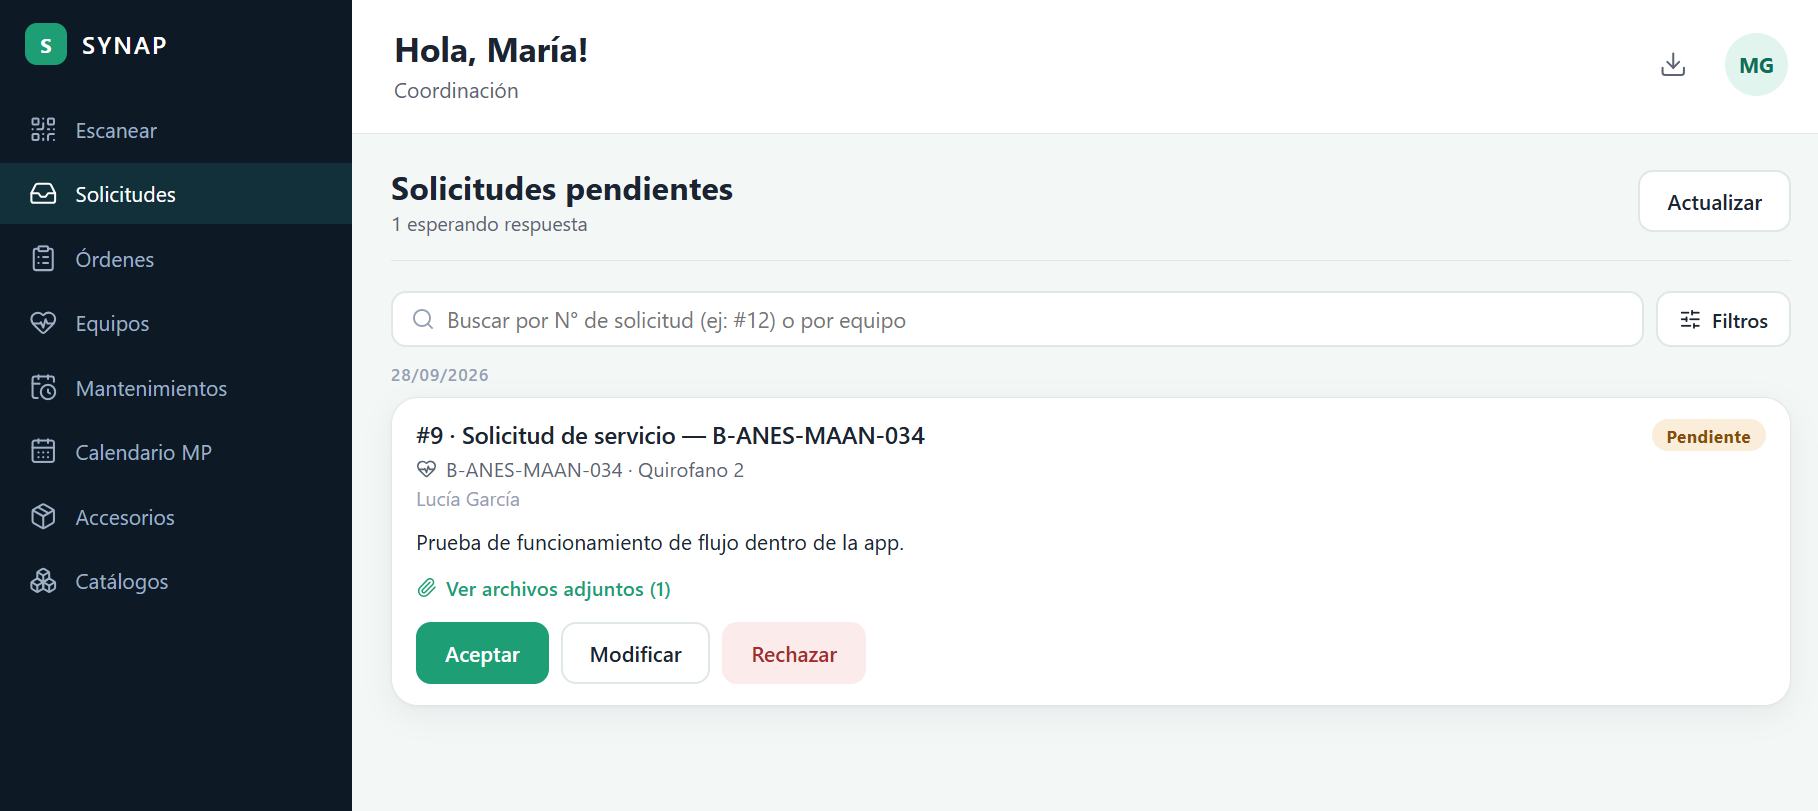
\includegraphics[width=\linewidth,height=0.45\textheight,keepaspectratio]{fotos/Figura_4_16_solicitudes_coordinacion.png}
    \caption{Pestaña “Solicitudes” de coordinación.}
    \label{fig:solicitudes-coord}
\end{figure}

\subsubsection{Órdenes de trabajo}
\label{sec:ordenes-trabajo}
La orden de trabajo registra cada intervención sobre un equipo y es la entidad en la que convergen los demás módulos. Nace de una solicitud aceptada (sección~\ref{sec:solicitudes}), de una falla detectada durante un preventivo o de la generación automática de preventivos (sección~\ref{sec:mantenimiento-preventivo}), y se identifica con un número correlativo, como OT-0037. Sus estados se describieron en la sección~\ref{sec:estados}.

\noindent \textbf{Listado y visibilidad por perfil.} Cada perfil ve las órdenes que le corresponden:

\begin{itemize}
    \item \textbf{Técnico.} La pestaña “Mis órdenes” muestra las asignadas a su nombre y las de su grupo que todavía no tienen técnico: las preventivas recién generadas y las correctivas aceptadas sin responsable. No aparecen las asignadas a sus compañeros.
    \item \textbf{Coordinación.} La pestaña “Órdenes” muestra las de los grupos que tiene a cargo. El filtro “Sin asignar” funciona como su bandeja de pendientes, ya que repartir el trabajo es una tarea propia de este perfil.
    \item \textbf{Jefatura.} La pestaña “Órdenes” muestra las de todos los grupos, solo para consulta: ve el detalle completo, pero ninguna acción que modifique la orden, y el backend rechaza sus intentos de asignarla, editarla, completarla, cerrarla o registrar consumos en ella aunque se hagan por fuera de la interfaz (sección~\ref{sec:backend-bd}).
\end{itemize}
En todos los casos el listado se filtra por estado, tipo, prioridad y fecha de notificación, y se busca por número de orden o por código de equipo. La búsqueda por número admite variantes (“37”, “OT 37” u “OT-037”), de modo que nadie tenga que recordar el formato exacto. Las preventivas se distinguen de las correctivas con una etiqueta y un borde de color (Figura~\ref{fig:mis-ordenes}).

\begin{figure}[H]
    \centering
    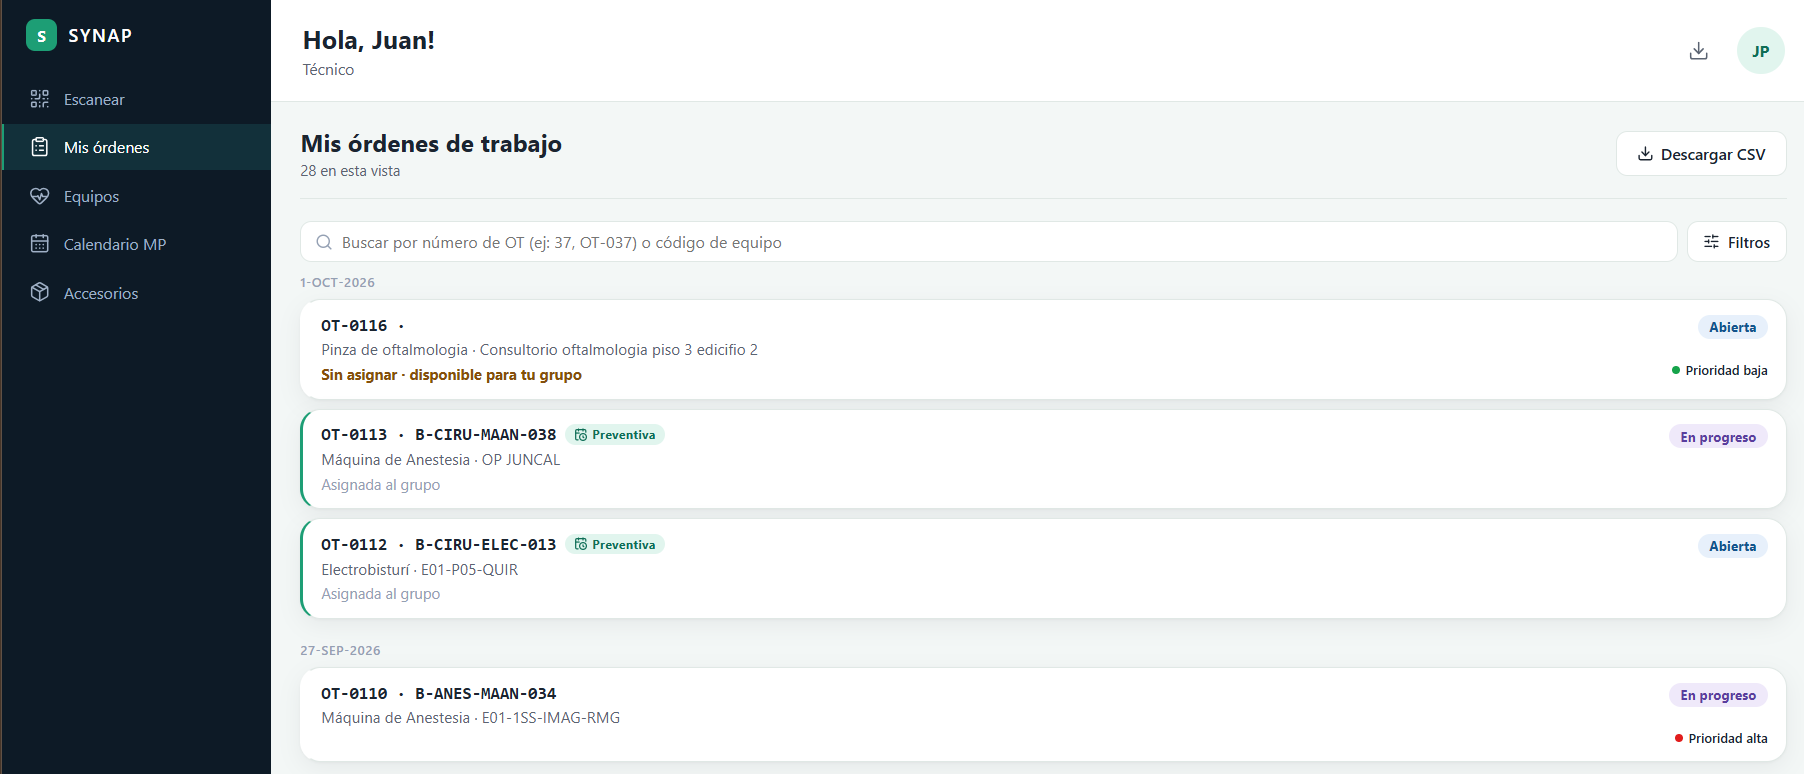
\includegraphics[width=\linewidth,height=0.45\textheight,keepaspectratio]{fotos/Figura_4_17_mis_ordenes_tecnico.png}
    \caption{Pestaña “Mis órdenes” del técnico.}
    \label{fig:mis-ordenes}
\end{figure}

\noindent \textbf{Detalle de una orden.} Reúne los datos del equipo y su criticidad, el tipo, la prioridad y el estado, quién reportó la falla, a quién está asignada y quién la inició y la cerró, con sus fechas (Figura~\ref{fig:detalle-orden}). Una correctiva generada durante un preventivo indica la orden de origen, y si proviene de una solicitud con fotos o documentos, estos se muestran en “Archivos adjuntos”. Desde el detalle se realizan las siguientes acciones:

\begin{itemize}
    \item \textbf{Asignar o reasignar.} Coordinación asigna una correctiva a un integrante del grupo de la orden con “Asignar / Reasignar técnico”. Un técnico del grupo puede hacer lo mismo para pasársela a un compañero, o tomar una orden sin asignar con “Tomar esta orden”. Las preventivas pertenecen al grupo y no se asignan a una persona.
    \item \textbf{Empezar a trabajar.} Pasa la orden a en progreso y registra quién la inició y cuándo. En una correctiva lo hace el técnico asignado, al igual que la parada del equipo y el consumo de accesorios; en una preventiva, quien la toma (sección~\ref{sec:mantenimiento-preventivo}).
    \item \textbf{Parada del equipo.} Los botones “Iniciar parada del equipo” y “Finalizar parada del equipo” registran el tiempo en que el equipo estuvo efectivamente fuera de servicio, y mientras está en curso la orden muestra el aviso “Equipo parado momentáneamente”. Una orden admite varias paradas y el sistema acumula el total.
    \item \textbf{Bitácora.} Registra el avance con entradas firmadas con su autor, fecha y hora, por ejemplo “se pidió el repuesto, llega en dos días”. A diferencia del campo de observaciones, que resume el cierre, conserva la secuencia de lo ocurrido. Escriben los técnicos del grupo y su coordinación.
    \item \textbf{Editar orden.} Mientras no esté cerrada, permite corregir la descripción, la prioridad y el equipo asociado, por ejemplo cuando la solicitud se cargó con un equipo equivocado, con una confirmación previa. Si el nuevo equipo pertenece a otro grupo, la orden pasa a ese grupo y, si el técnico asignado no pertenece a él, queda sin asignar. En las correctivas, coordinación puede además corregir la clasificación de la falla (sección~\ref{sec:estados}). Pueden editarla los técnicos del grupo y coordinación.
    \item \textbf{Registrar consumo de accesorios.} Descuenta del stock lo utilizado en la intervención (sección~\ref{sec:stock}).
\end{itemize}
\begin{figure}[H]
    \centering
    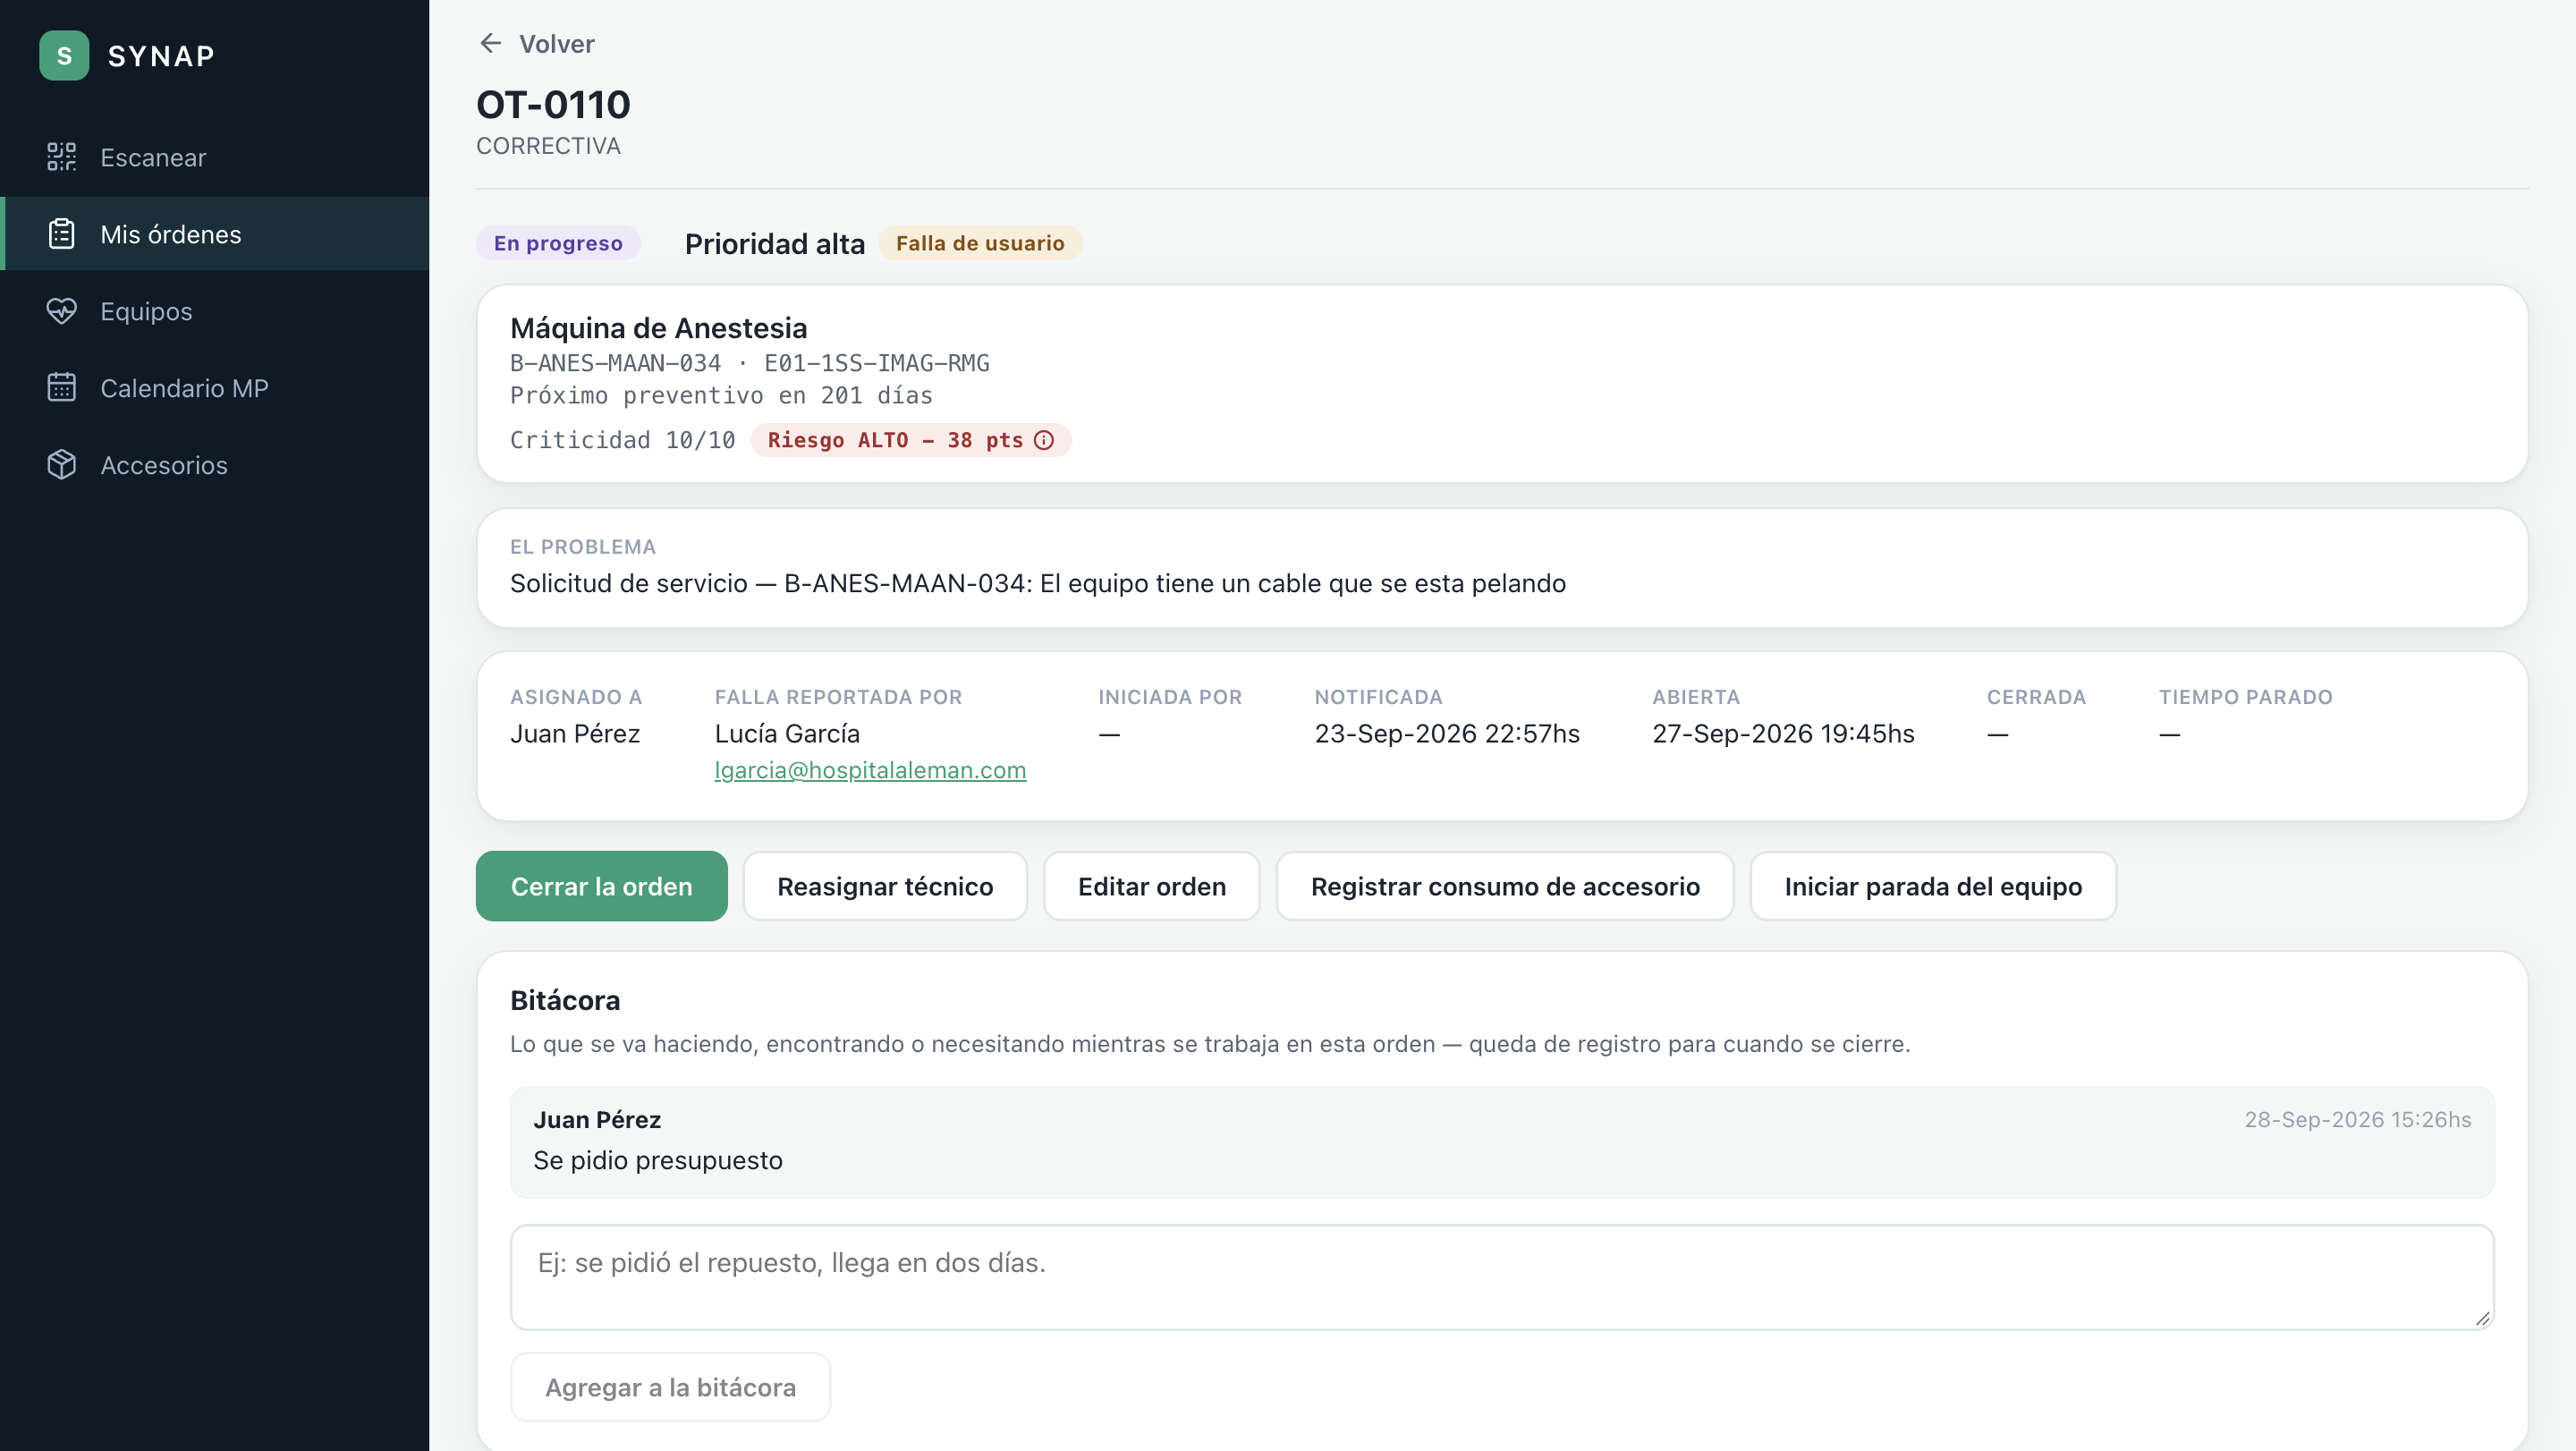
\includegraphics[width=\linewidth,height=0.45\textheight,keepaspectratio]{fotos/Figura_4_18_detalle_orden_correctiva.png}
    \caption{Detalle de una orden correctiva, vista del técnico.}
    \label{fig:detalle-orden}
\end{figure}

\noindent \textbf{Cierre de una correctiva.} La cierra el técnico asignado o la coordinación del grupo con el botón “Cerrar la orden”, completando el campo “Qué se hizo”, que queda en el historial del equipo.  Si al cerrar una correctiva, o al completar una preventiva, queda una parada sin finalizar, el sistema la finaliza con esa fecha para que no distorsione el tiempo de inactividad. Las preventivas siguen otro circuito (sección~\ref{sec:mantenimiento-preventivo}).
\subsubsection{Mantenimientos preventivos}
\label{sec:mantenimiento-preventivo}
Este módulo incorpora al sistema el circuito completo del mantenimiento preventivo, desde la definición de los planes hasta el informe del mantenimiento realizado

\textbf{Planes y checklists.} Se administran desde la pestaña “Mantenimientos”, disponible para coordinación y jefatura, ya que definir los planes es una tarea de gestión y no de ejecución. Allí se listan los checklists, con el de cada tipo de equipo y el genérico, que se aplica a los tipos sin checklist propio. “Nuevo checklist” pide el nombre, una descripción opcional, el tipo de equipo (o la marca de genérico), la frecuencia sugerida en días y los ítems, cada uno obligatorio u opcional; al guardar, el sistema suma los dos ítems fijos de la sección~\ref{sec:modelo-datos}. “Editar checklist” permite modificarlo, salvo esos dos ítems, y los ítems quitados se dan de baja sin borrarse, por lo que las respuestas ya registradas se conservan. Para evitar que un tipo de equipo quede sin protocolo, una de las faltas señaladas en la encuesta, al crear un tipo nuevo en “Catálogos” el sistema ofrece crear su checklist en ese momento, con el tipo ya seleccionado.

\textbf{Programación de cada equipo.} Un equipo se incorpora al plan al darlo de alta, con la casilla “Programar mantenimiento preventivo” (sección~\ref{sec:activos-qr}). Para uno que todavía no tiene mantenimiento, como los de la migración (sección~\ref{sec:integracion-datos}), coordinación usa en la ficha el botón “Asignar mantenimiento preventivo”, eligiendo el plan y el mes de la primera orden. Si ya lo tiene, “Reprogramar” mueve el mes del próximo preventivo sin modificar el plan ni la frecuencia.

\textbf{Generación automática de las órdenes.} La tarea programada (sección~\ref{sec:backend-bd}) crea una orden preventiva abierta, asignada al grupo responsable y vinculada a su checklist, para cada equipo cuyo próximo mantenimiento vence en el mes en curso o antes, excepto los dados de baja y los que ya tienen una preventiva sin cerrar. En el mismo paso calcula la fecha del ciclo siguiente, sumando la frecuencia del equipo. Como la reprogramación se hace al generar la orden y no al cerrarla, un mantenimiento completado con retraso no desplaza el resto del calendario.

\textbf{Calendario de mantenimientos.} La pestaña “Calendario MP”, disponible para técnicos, coordinación y jefatura, reemplaza a las planillas de cada grupo (Figura~\ref{fig:calendario-mp}). Muestra, mes a mes, los mantenimientos programados, que pueden estar generados, con el número y el estado de la orden, o en pronóstico, cuando la orden todavía no existe, algo habitual en los meses futuros. Los primeros llevan al detalle de la orden y los segundos, a la ficha del equipo. La lista se filtra por equipo, estado y grupo, y el gráfico “Carga de mantenimientos por mes” resalta el mes más cargado, lo que permite redistribuir el trabajo con anticipación. Coordinación y jefatura disponen además de “Generar ahora”, para forzar la generación sin esperar a la tarea diaria.

\begin{figure}[H]
    \centering
    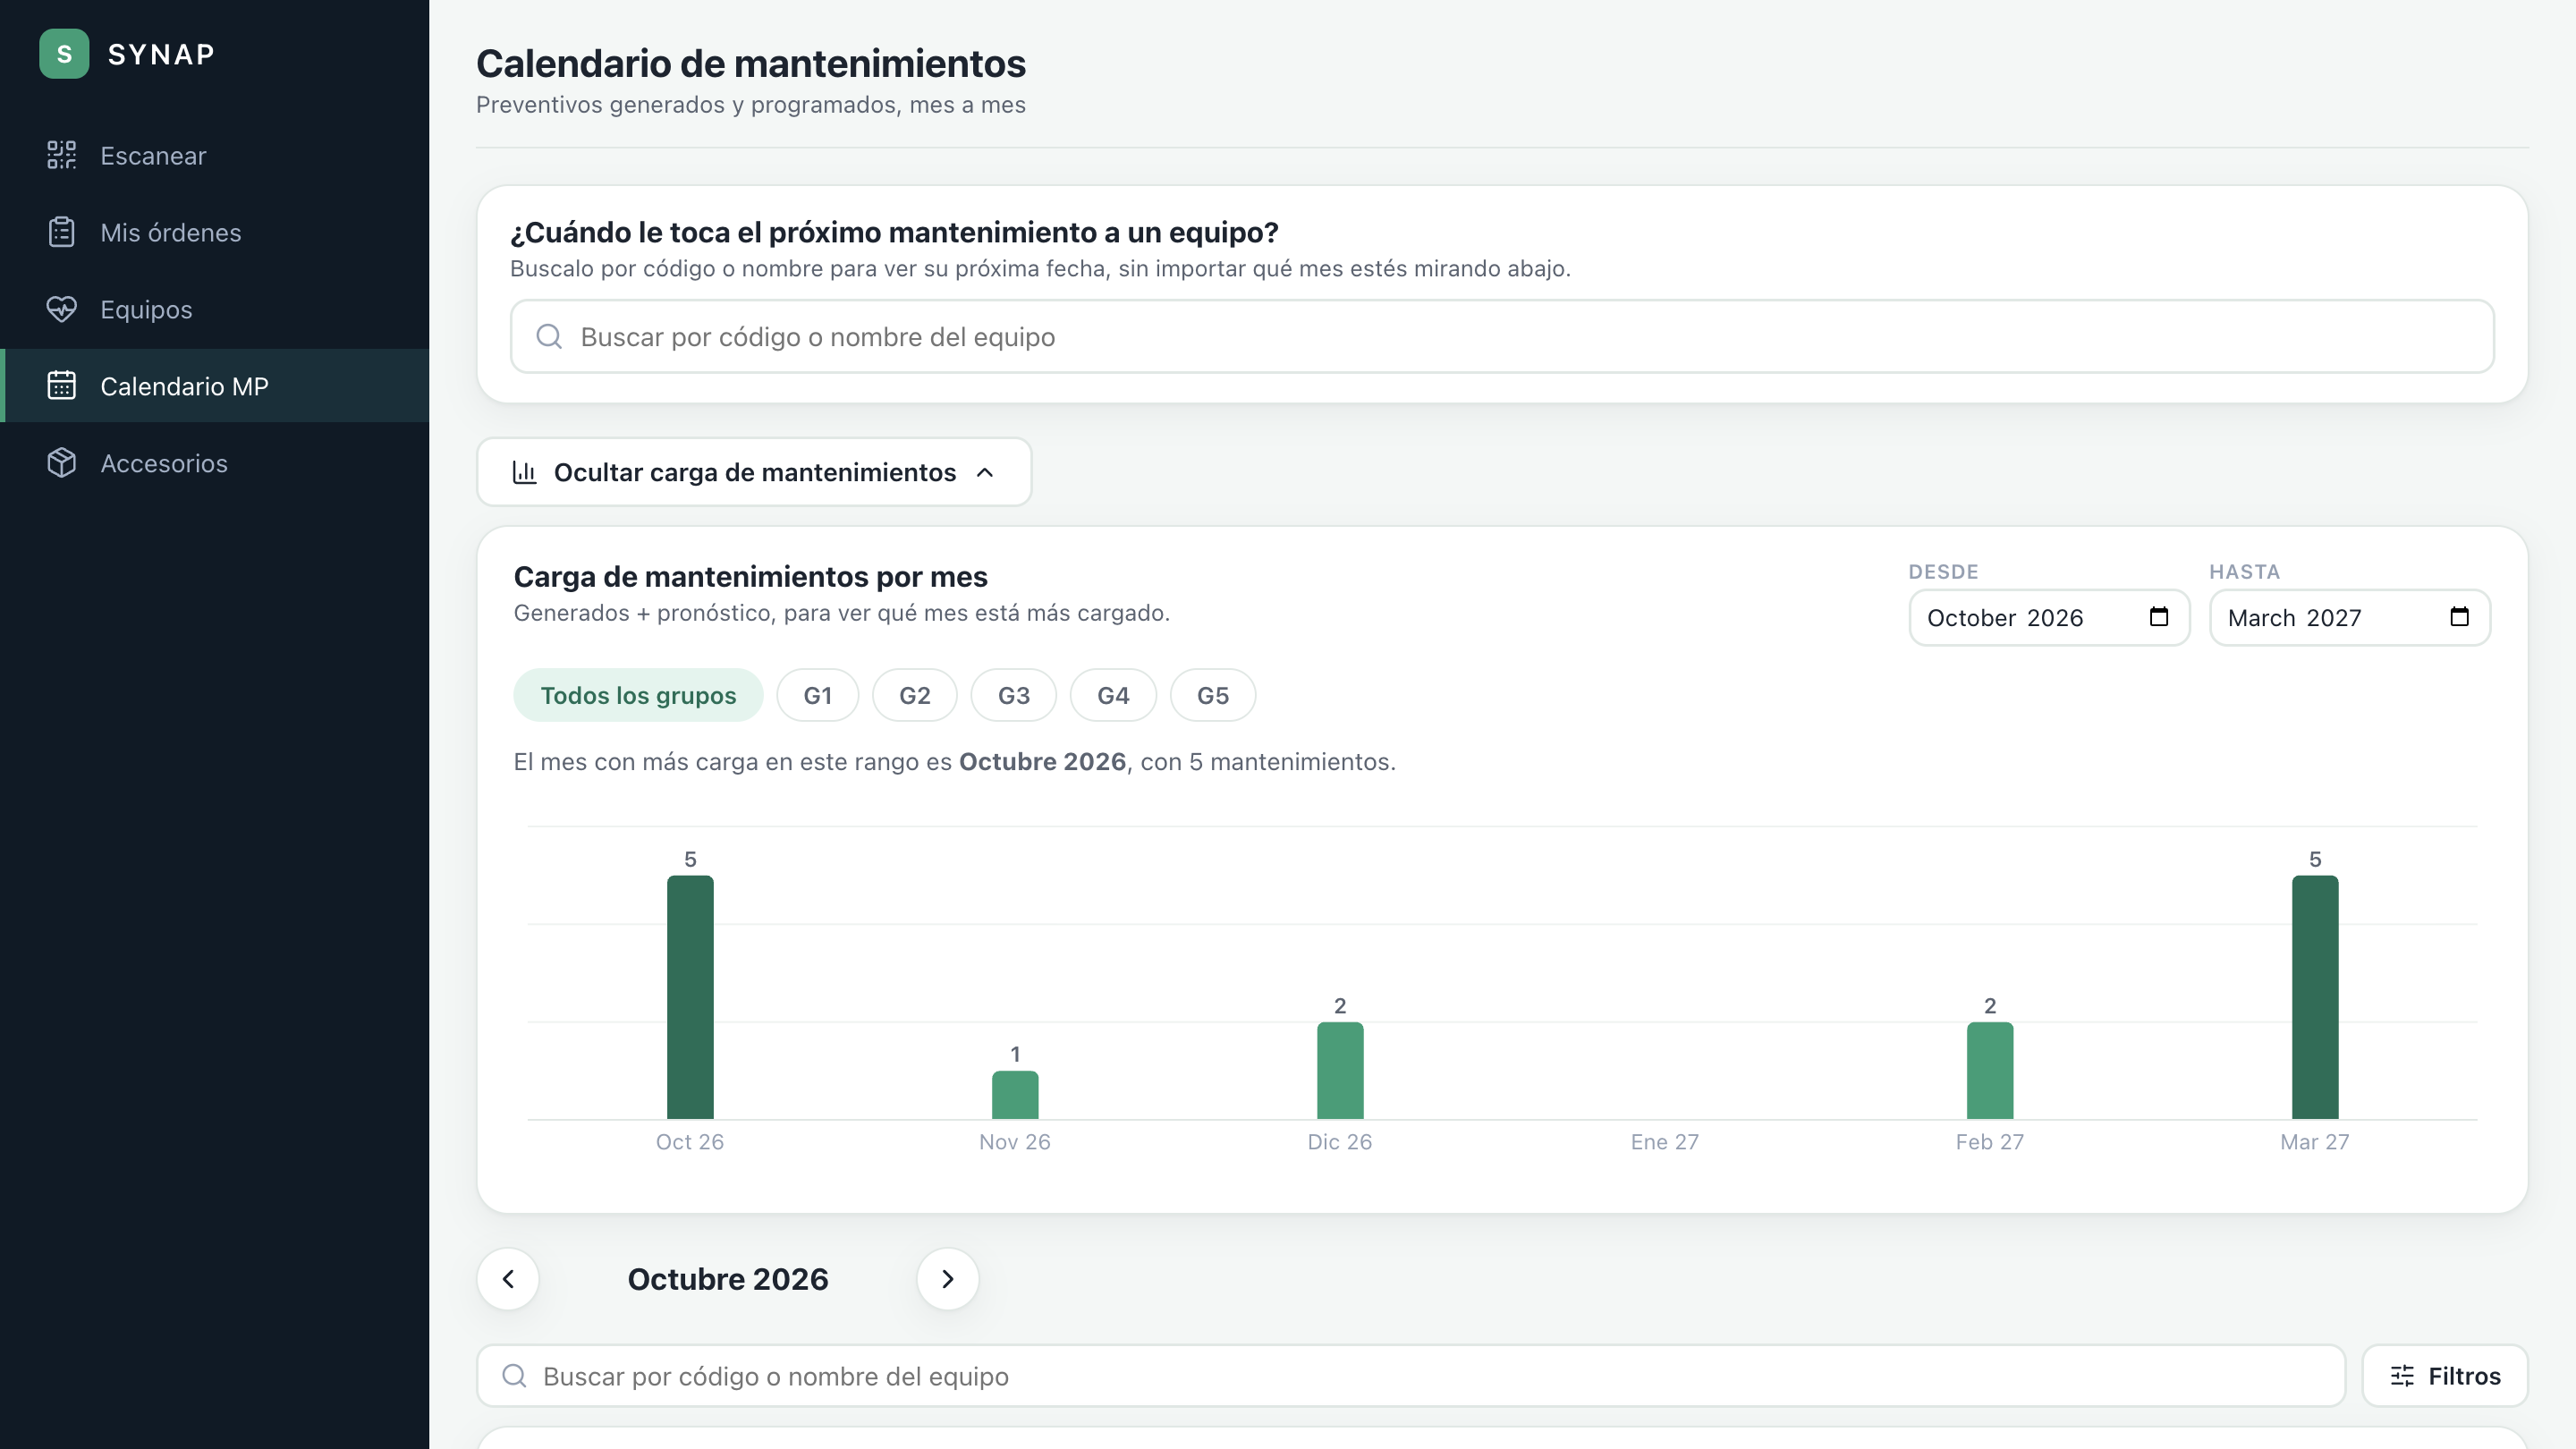
\includegraphics[width=\linewidth,height=0.45\textheight,keepaspectratio]{fotos/Figura_4_19_calendario_mp.png}
    \caption{Pestaña “Calendario MP”.}
    \label{fig:calendario-mp}
\end{figure}

\textbf{Ejecución del checklist.} Cualquier técnico del grupo, o su coordinación, puede iniciar una preventiva con “Empezar a trabajar”; desde entonces solo esa persona puede trabajarla, y el resto del grupo puede verla pero no modificarla. En la sección “Checklist de mantenimiento” (Figura~\ref{fig:checklist}) cada ítem se responde con “Pasa” o “No pasa” (“Sí” o “No” en “Necesidad de correctivo”, para que la pregunta se entienda). Con “No pasa” se describe el problema en “Qué encontraste” y se puede “Generar una orden correctiva por esto”, opción marcada por defecto y con prioridad opcional, que queda vinculada a la preventiva y asignada a quien realiza el mantenimiento. “Cambiar” corrige una respuesta ya cargada, y “Algo no funciona: generar correctiva” abre una correctiva por un problema que no corresponde a ningún ítem. Las correctivas generadas se listan en la misma orden.

\begin{figure}[H]
    \centering
    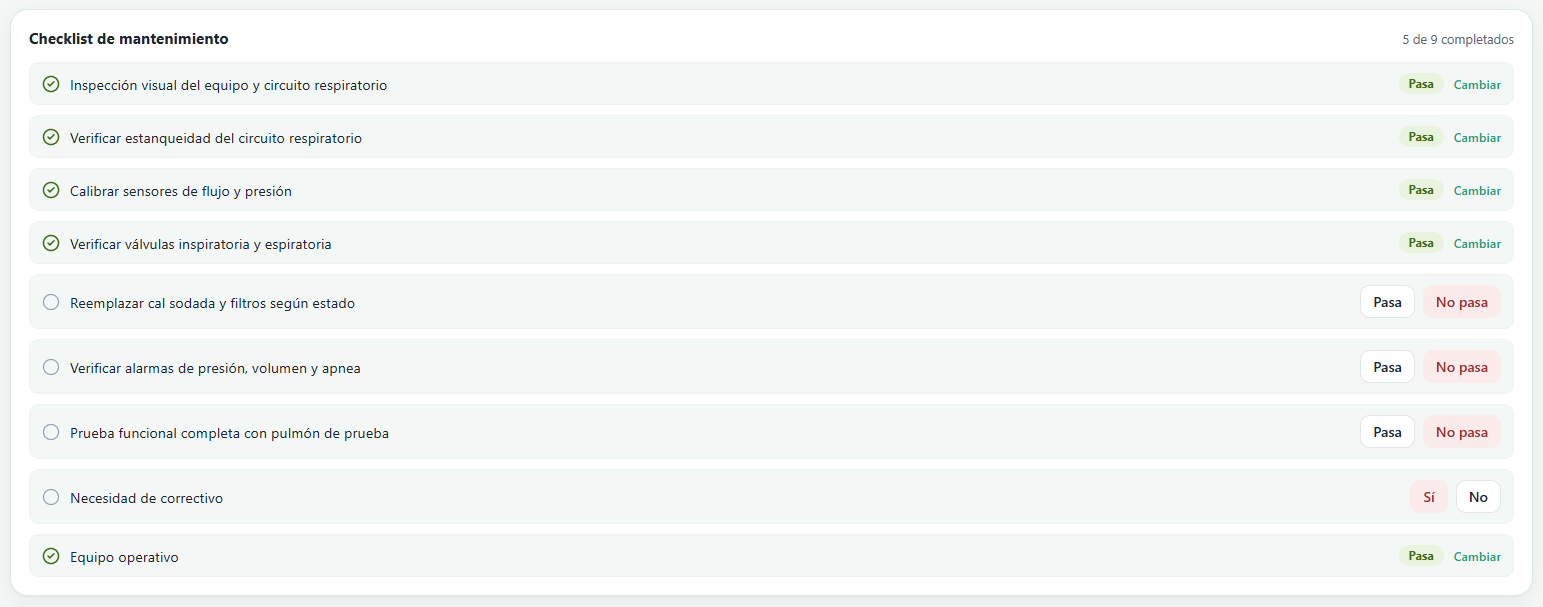
\includegraphics[width=\linewidth,height=0.40\textheight,keepaspectratio]{fotos/Figura_4_20_checklist_mantenimiento.png}
    \caption{Sección “Checklist de mantenimiento” de una orden preventiva en curso, con ítems respondidos y pendientes.}
    \label{fig:checklist}
\end{figure}

\textbf{Completar y autorizar.} Al responder los ítems obligatorios, una ventana resume las respuestas antes de completar la orden. Solo se pide un texto adicional cuando hace falta justificar un retraso, porque cada ítem ya registra su observación. A partir de ahí, la orden sigue el circuito de revisión de coordinación descrito en el apartado~\ref{sec:estados}.

\textbf{Informe de mantenimiento.} Una vez cerrada la orden, el botón “Descargar informe PDF” genera un informe con los datos del equipo y de la orden, quién la inició y quién la cerró, el motivo del retraso si lo hubo, y el resultado y la observación de cada ítem. Está pensado para reemplazar al registro en papel de la carpeta del equipo.

\subsubsection{Stock de accesorios y repuestos}
\label{sec:stock}

Este módulo lleva el stock de accesorios y repuestos y lo vincula con las órdenes de trabajo en las que se consumen, de modo que un equipo no quede fuera de servicio por un faltante que nadie registró (sección~\ref{sec:inventario}). Responde a un pedido de la encuesta (sección~\ref{sec:encuesta}).

\textbf{Consulta.} La pestaña “Accesorios”, disponible para técnicos, coordinación y jefatura, lista cada accesorio con su código, su stock actual y sus umbrales, y lo identifica con un color según su nivel:
\begin{itemize}
    \item Stock ok (verde). La cantidad supera el punto de reposición.
    \item Conviene reponer (amarillo). La cantidad llegó al punto de reposición o bajó de él, por lo que conviene iniciar una compra.
    \item Stock crítico (rojo). La cantidad llegó al stock mínimo o bajó de él.
\end{itemize}

La lista se busca por nombre, código o descripción, se filtra por el tipo de equipo al que corresponde cada accesorio (incluidos los de uso general, como guantes o alcohol en gel) y puede limitarse a los que requieren atención. El botón “Ver historial” lleva al historial de movimientos, al final de la pantalla (Figura~\ref{fig:accesorios}).

\begin{figure}[H]
    \centering
    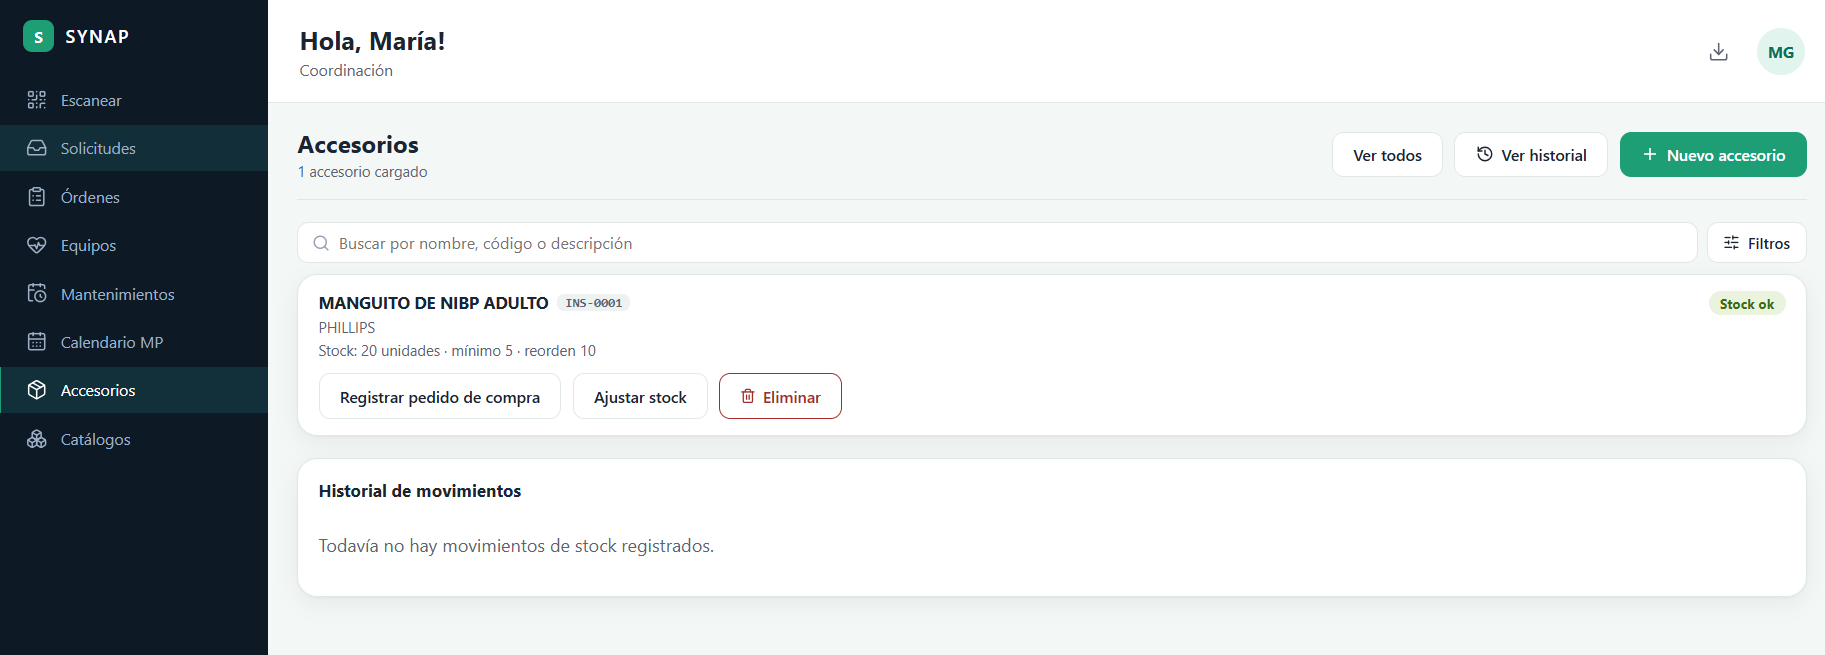
\includegraphics[width=\linewidth,height=0.45\textheight,keepaspectratio]{fotos/Figura_4_21_accesorios.png}
    \caption{Pestaña “Accesorios”.}
    \label{fig:accesorios}
\end{figure}

\textbf{Alta y eliminación.} Por ser una tarea de catálogo, el botón “Nuevo accesorio” está disponible solo para coordinación y jefatura. Pide el nombre (obligatorio), la descripción, la unidad y el tipo de equipo (opcionales) y los valores de stock actual, mínimo y punto de reposición. El código lo asigna el sistema con el formato INS-0001. Un accesorio cargado por error puede eliminarse, pero solo si todavía no tiene movimientos, para no perder historial.

\textbf{Compras.} Siguiendo el circuito real del hospital, una compra se registra en dos pasos. Con “Registrar pedido de compra” se indican la cantidad y, de manera opcional, el proveedor y el número de orden de compra; el accesorio pasa a mostrar “Pedido en camino”, pero su stock no cambia. Cuando el pedido llega, “Marcar recibida” suma la cantidad al stock. Así el sistema no cuenta como disponible un repuesto que todavía no llegó y evita pedirlo dos veces.

\textbf{Consumo desde las órdenes de trabajo.} Se registra en el detalle de una orden, preventiva o correctiva, con el botón “Registrar consumo de accesorio”: se elige el accesorio y la cantidad, y el consumo queda listado en “Accesorios consumidos en esta OT”, asociado a esa intervención, a ese equipo y a quien lo cargó. Solo puede registrarlo quien está trabajando la orden, y no es posible una vez cerrada; jefatura, que consulta las órdenes pero no las opera, no puede hacerlo. El consumo nunca se rechaza por falta de stock, aunque este quede por debajo del mínimo o incluso en negativo, porque el accesorio ya se usó y bloquear el registro solo dejaría el consumo sin documentar; una diferencia de este tipo puede regularizarse luego con un ajuste. En su lugar, el sistema avisa en pantalla si el accesorio quedó en “Conviene reponer” o en “Stock crítico”. 

\textbf{Ajustes e historial.} Para las diferencias que surgen fuera de una orden, como una rotura, una merma o un conteo físico que no coincide con el sistema, el botón “Ajustar stock” registra una entrada o una salida con su cantidad y un motivo obligatorio. Al final de la pantalla, el historial reúne las compras recibidas, los consumos y los ajustes, del más reciente al más antiguo, y permite seguir los cambios recientes de cada accesorio. Muestra los 100 movimientos más recientes; consultar los anteriores queda como mejora futura.

\subsubsection{Notificaciones automáticas}
\label{sec:notificaciones}
Las notificaciones fueron la funcionalidad que más dividió a los encuestados (sección~\ref{sec:encuesta}), por lo que se plantearon como un objetivo de máxima. Para no saturar a nadie, todos los avisos se envían por correo a una única casilla del servicio y no al correo personal de cada integrante, de modo que quedan centralizados y cada grupo los consulta cuando lo necesita. Tres situaciones generan un aviso:
\begin{itemize}
\item \textbf{Orden correctiva creada.} Se envía cada vez que se abre una correctiva: al aceptar una solicitud de servicio (sección~\ref{sec:solicitudes}) o al generarla desde un preventivo (sección~\ref{sec:mantenimiento-preventivo}), ya sea por un ítem del checklist o con el botón “Algo no funciona”. Indica el número de la orden, el equipo, la descripción del problema y el grupo asignado. 
\item \textbf{Stock crítico.} Se envía cuando un consumo o un ajuste de salida hace que un accesorio pase a nivel crítico, con la cantidad restante y la orden o el motivo que lo originó. Si ya estaba en ese nivel no se repite, para no llenar la casilla con un aviso por cada movimiento. El nivel “Conviene reponer” no genera aviso, porque es una alerta más leve que ya se ve en la pestaña “Accesorios”. 
\item \textbf{Mantenimiento próximo a vencer.} Una tarea programada (sección~\ref{sec:backend-bd}) revisa todos los días si comenzó la última semana del mes y, de ser así, reúne en un único correo, con el equipo y la fecha programada de cada uno, los mantenimientos del mes que todavía no se realizaron. Cada mantenimiento se avisa una sola vez, para que el aviso no se repita todos los días de esa semana.
\end{itemize}

Los avisos son únicamente por correo, ya que el sistema no cuenta con notificaciones dentro de la aplicación. El envío se describió en la sección~\ref{sec:backend-bd}.

\subsubsection{Panel de indicadores}
\label{sec:panel-indicadores}
El panel de indicadores responde a la dificultad para obtener informes del sistema actual, el tema más repetido en la encuesta (sección~\ref{sec:encuesta}), y materializa los indicadores de la sección~\ref{sec:indicadores-gestion}. Se accede desde la pestaña “Dashboard” (Figura~\ref{fig:panel-indicadores}), disponible solo para jefatura, y todos los valores se calculan en el momento de abrir la pantalla con los datos registrados, sin necesidad de armar informes por fuera del sistema.

Dos criterios rigen el panel. El primero es que un porcentaje o un promedio sin datos suficientes muestra “Sin datos” y nunca un cero: un cumplimiento del 0 % y la ausencia de preventivos cargados significan cosas opuestas, y confundirlos podría llevar a decisiones equivocadas sobre el parque. El segundo es que los indicadores de falla (tiempo fuera de servicio, cantidad de fallas, tiempo medio de reparación y tiempo medio entre fallas) miden la confiabilidad de los equipos, por lo que no incluyen las fallas de usuario ni las órdenes sin un equipo asociado, como las de instrumental, que no pueden atribuirse a ninguno. Todas ellas sí cuentan como trabajo del servicio en las órdenes totales y en la carga por grupo (sección~\ref{sec:estados}); solo las órdenes sin equipo quedan fuera cuando se filtra por grupo o por tipo, porque el filtro opera sobre equipos. 

En la parte superior, los filtros “Grupo técnico” y “Tipo de equipo” recalculan los indicadores solo sobre los equipos que coinciden. Funcionan en cascada: al elegir un grupo, la lista de tipos muestra solo los que ese grupo atiende. El gráfico de mantenimientos planeados respeta únicamente el filtro de grupo. Los indicadores se organizan en los siguientes bloques:

\begin{itemize}
    \item \textbf{Alertas y pendientes.} Las órdenes abiertas sin técnico asignado y los preventivos vencidos, es decir, aquellos cuyo mes programado ya pasó sin que se realizaran.
    \item \textbf{Estado del parque hoy.} Los equipos registrados, las órdenes abiertas sobre el total y el cumplimiento de los preventivos, que es el porcentaje de los mantenimientos generados que se realizaron dentro del mes programado (sección~\ref{sec:estados}) y puede consultarse para un mes puntual.
    \item \textbf{Tiempos y desempeño.} El tiempo fuera de servicio, promedio por correctiva cerrada a partir de las paradas medidas; el tiempo medio de reparación (MTTR), desde la apertura hasta el cierre de las correctivas; y la cantidad de fallas registradas.
    \item \textbf{Estado y carga de trabajo.} Tres gráficos: la distribución de las órdenes por estado, las órdenes abiertas por grupo técnico, que muestra cómo se reparte la carga del servicio, y la distribución de los equipos según su vida útil (sección~\ref{sec:criticidad-riesgo}).
    \item \textbf{Mantenimientos planeados.} La cantidad de mantenimientos del mes actual y de los cinco siguientes, contando los ya generados y los pronosticados.
    \item \textbf{Fallas por trimestre.} La evolución de las fallas en los últimos cuatro trimestres, incluido el actual.
    \item \textbf{Equipos con más fallas.} Los diez equipos que más fallaron, candidatos a revisar o reemplazar. Al seleccionar uno, se accede a su ficha.
    \item \textbf{Fallas por urgencia.} La distribución de las fallas según la prioridad de su orden correctiva: baja, media, alta, crítica o sin prioridad.
    \item \textbf{Equipos menos confiables.} Los equipos ordenados por tiempo medio entre fallas (MTBF), de modo que los que fallan más seguido aparecen primero. En línea con la sección~\ref{sec:indicadores-gestion}, solo se calcula para equipos con al menos dos fallas registradas. Al seleccionar uno, se accede a su ficha.
\end{itemize}

\begin{figure}[H]
    \centering
    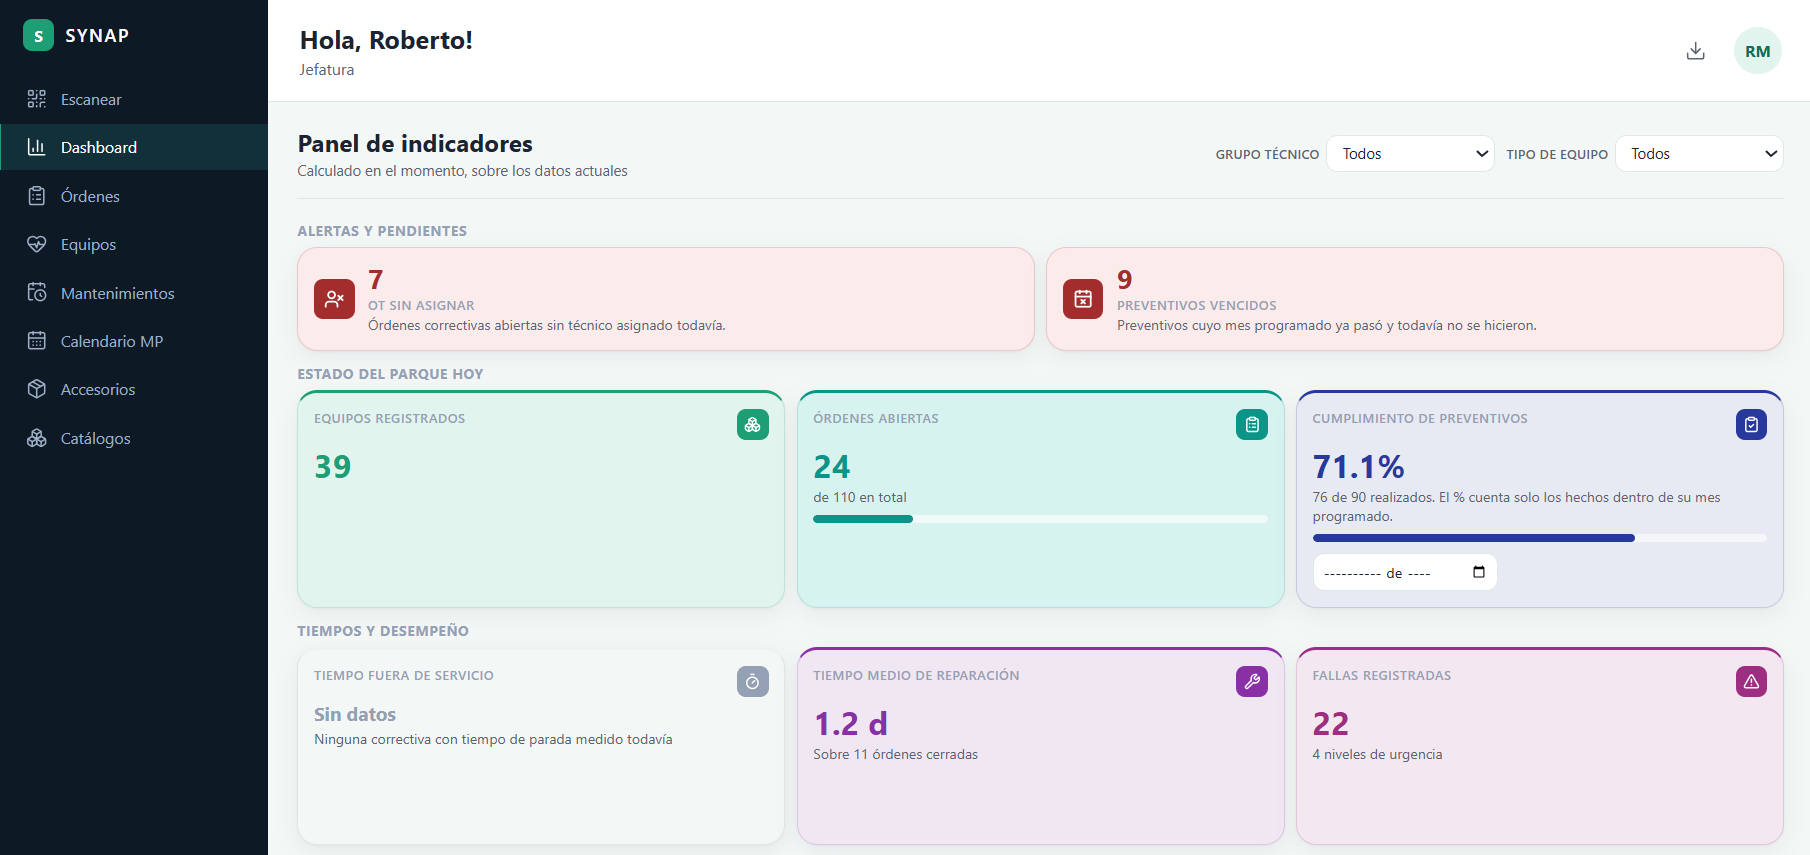
\includegraphics[width=\linewidth,height=0.45\textheight,keepaspectratio]{fotos/Figura_4_22_panel_indicadores.png}
    \caption{Panel de indicadores, vista de jefatura.}
    \label{fig:panel-indicadores}
\end{figure}

Así, jefatura puede pasar de una vista general del servicio a un equipo puntual en pocos pasos, con información concreta para decisiones como la revisión de un plan de mantenimiento o el recambio de un equipo.

\subsubsection{Descarga de datos}
\label{sec:descarga-datos}
La encuesta (sección~\ref{sec:encuesta}) mostró que, cuando el sistema actual no ofrece la información que el servicio necesita, el personal la exporta y sigue trabajando sobre ella por fuera. Para responder a esa práctica, SYNAP permite descargar en formato CSV los listados de equipos, órdenes de trabajo, mantenimientos (preventivos y correctivos) y accesorios, disponibles para técnicos, coordinación y jefatura. El ícono de descarga del encabezado baja cada listado completo, y las pantallas de equipos y de órdenes tienen además un botón “Descargar CSV” que respeta la búsqueda y los filtros aplicados en pantalla. El listado de equipos incluye, además de los datos de la ficha y las fechas de mantenimiento, la criticidad, el nivel de riesgo y el puntaje del cálculo descrito en la sección~\ref{sec:criticidad-riesgo} para los equipos médicos con datos suficientes.

Las descargas de órdenes y de mantenimientos se limitan al alcance de cada perfil: el grupo del técnico, los grupos a cargo de coordinación o todos los grupos, en el caso de jefatura. Los archivos están preparados para abrirse directamente en Excel en español, con punto y coma como separador, tildes bien codificadas y fechas en formato día/mes/año. De este modo, el análisis por fuera del sistema parte de datos vigentes y no de copias armadas a mano.

\subsection{Integración de los datos del hospital}
\label{sec:integracion-datos}
Para validar el funcionamiento del sistema en un caso de uso real, tal como plantea el último de los objetivos de mínima (sección~\ref{sec:objetivos-minima}), se incorporaron los datos reales del servicio de Bioingeniería del Hospital Alemán. Hasta ese momento se había trabajado con la base ficticia descrita en la sección~\ref{sec:datos-prueba}. Esta sección muestra cómo se comporta SYNAP con la información de la institución y qué ajustes se necesitaron.

\subsubsection{Criterios de la migración}
Los datos reales se cargaron en una base de datos separada de la de prueba, con la misma estructura y el mismo código de aplicación. Para pasar de una base a otra alcanza con cambiar un parámetro de conexión. Así, la base de prueba siguió intacta y la información del hospital nunca se mezcló con los datos de desarrollo.

Antes de cargar nada, se compararon las exportaciones de Maximo analizadas en la sección~\ref{sec:analisis-maximo} con el modelo de datos de SYNAP, para detectar de antemano qué había que adaptar. Después, la carga se hizo desde el editor SQL y el editor de tablas de la plataforma de base de datos.

A lo largo de la migración se tomaron tres decisiones:

\begin{enumerate}
    \item Se dejaron afuera 120 registros que no son equipos. Maximo los usa para canalizar pedidos que no se refieren a un equipo concreto, como los “pedidos a Bioingeniería” de cada servicio. En SYNAP no hacen falta, porque una solicitud puede registrarse sin asociarla a un equipo.
    \item Se armó el catálogo de tipos de equipo a partir de las descripciones de Maximo. Resultaron 358 tipos, y 46 tenían un nombre ambiguo. Ocho se corrigieron consultando la descripción original, y los demás quedaron con el nombre obtenido, que se puede editar desde la aplicación.
    \item Las cuentas de usuario replican la estructura del personal del servicio, con el perfil asignado según el cargo, es decir, jefatura para la jefa de Bioingeniería, coordinación para los coordinadores y técnico para el resto del personal, incluidos los bioingenieros. Para resguardar los datos personales, en la base del prototipo se utilizan usuarios ficticios, con nombre, número de usuario y correo inventados, que conservan la misma cantidad de personas y la misma distribución en roles y grupos. Las cuentas se cargan sin contraseña y cada persona crea la suya al activarla.
\end{enumerate}

\subsubsection{Datos incorporados}
La Tabla~\ref{tab:datos-incorporados} resume lo que quedó cargado. El inventario exportado reunía 6.302 registros. Al descontar las 120 entradas genéricas quedan 6.182 equipos, de los cuales se migraron 6.178. Los cuatro restantes tenían estados sin equivalente en el sistema (“No listo” y “Falta”).

\begin{table}[H]
    \caption{Datos del Hospital Alemán incorporados a SYNAP.}
    \label{tab:datos-incorporados}
    \centering
    \renewcommand{\arraystretch}{1.5}
    \begin{tabular*}{\linewidth}{@{\extracolsep{\fill}}lcl@{}}
        \toprule
        \textbf{Tipo de dato} & \textbf{Cantidad} & \textbf{Observación} \\
        \midrule
        Sectores & 77 & Más un sector “sin sector” para los equipos sin ubicación \\
        Grupos de trabajo & 6 & G1 a G6; ningún equipo del inventario pertenece al Grupo 7 \\
        Tipos de equipos & 358 & 352 con grupo de trabajo asignado \\
        Equipos & 6.178 & 3.887 activos, 1.862 de baja y 429 inactivos \\
        Usuarios & 14 & Ficticios, con los roles y grupos del servicio \\
        \bottomrule
    \end{tabular*}
\end{table}

\subsubsection{Hallazgos de la prueba con datos reales}
\label{sec:hallazgos-datos-reales}
La base de prueba no permitía anticipar tres situaciones que aparecieron al trabajar con los datos reales:

\begin{itemize}
    \item Las cuentas no se podían activar. El número de identificación de los usuarios se había cargado sin la letra “u” inicial que exige el sistema. Se corrigió en la base de datos.
    \item La lista de equipos mostraba solo 200. Era el límite por defecto del sistema, que con la base ficticia no se notaba. Con más de 6.000 equipos, la lista pasó a dividirse en páginas de 50 (124 en total), ordenadas del equipo más nuevo al más viejo según su fecha de instalación.
    \item Los equipos no tenían mantenimiento preventivo. Los planes de mantenimiento de Maximo no se migraron, y hasta ese momento el sistema solo permitía asignar un plan al dar de alta un equipo nuevo. Se agregaron dos acciones en la ficha del equipo, disponibles solo para coordinación: asignar un plan y el mes de la primera orden a un equipo que no tiene uno, y reprogramar el mes del próximo preventivo en uno que ya lo tiene (sección~\ref{sec:mantenimiento-preventivo}).
\end{itemize}

Con esta carga, SYNAP opera con el inventario completo del hospital y con usuarios ficticios que replican los roles y grupos del servicio. La migración abarcó los equipos, sus catálogos y las cuentas de usuario. Los planes de mantenimiento y sus checklists quedan para definirse con el servicio al momento de la puesta en marcha (capítulo~\ref{sec:futuro}). 

\newpage
\section{Resultados}
\label{sec:resultados}

Este capítulo reúne los resultados del trabajo. Presenta el sistema obtenido, su funcionamiento con los datos del hospital y la valoración del servicio de Bioingeniería.

\subsection{Sistema obtenido}
\label{sec:sistema-obtenido}

El resultado del trabajo es SYNAP, un prototipo funcional de sistema web para la gestión del equipamiento médico del servicio de Bioingeniería. Se utiliza desde el navegador, tanto en computadoras como en celulares (sección~\ref{sec:arquitectura-tecnologias}), y ofrece cuatro perfiles de usuario, enfermería, técnico, coordinación y jefatura, cada uno con las pantallas y acciones que le corresponden (sección~\ref{sec:perfiles-usuario}). Además, se encuentra publicado y puede usarse desde cualquier navegador (sección~\ref{sec:despliegue}).

El sistema acompaña el recorrido de un equipo dentro del servicio. Enfermería reporta una falla escaneando el QR del equipo, y coordinación la clasifica y la convierte en una orden de trabajo asignada a un técnico. Los mantenimientos preventivos se generan cada mes a partir del plan de cada tipo de equipo, y jefatura cuenta con un panel de indicadores. Todo esto responde a los requerimientos relevados en el servicio (secciones~\ref{sec:casos-uso} y~\ref{sec:requerimientos-funcionales}), y su cumplimiento frente a los objetivos de la sección~\ref{sec:objetivos} se retoma en las conclusiones (capítulo~\ref{sec:conclusiones}).

\subsection{Integración de los datos del hospital}
\label{sec:integracion-resultados}

Para validar el sistema en un caso de uso real, tal como plantea el último de los objetivos de mínima (sección~\ref{sec:objetivos}), se incorporaron los datos del servicio de Bioingeniería del Hospital Alemán, cuya migración se describe en la sección~\ref{sec:integracion-datos}. SYNAP opera hoy con 6.178 equipos, 358 tipos de equipo, 77 sectores, 6 grupos de trabajo y 14 cuentas de usuario ficticias que replican los roles y grupos del servicio (Figura~\ref{fig:equipos-datos-reales}). La prueba con esos datos llevó a tres ajustes, relacionados con la activación de las cuentas, el volumen de la lista de equipos y la asignación de planes de mantenimiento preventivo (sección~\ref{sec:hallazgos-datos-reales}).

\begin{figure}[H]
    \centering
    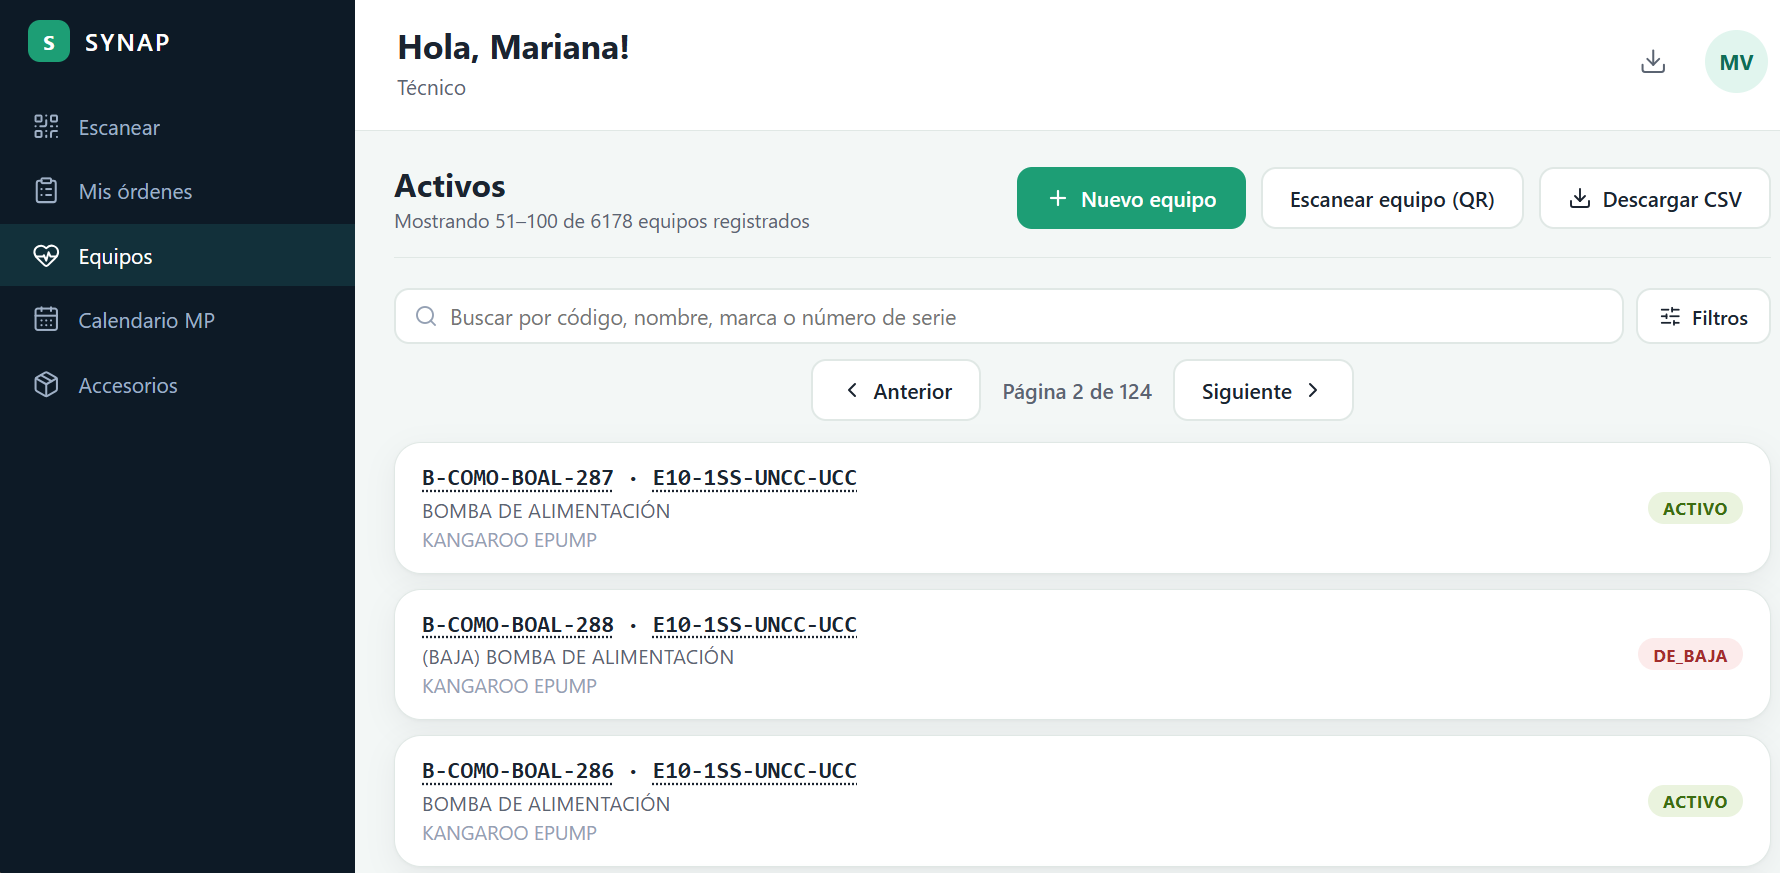
\includegraphics[width=\linewidth,height=0.45\textheight,keepaspectratio]{fotos/Figura_5_1_equipos_datos_reales.png}
    \caption{Pestaña “Equipos” con el inventario del Hospital Alemán incorporado a SYNAP.}
    \label{fig:equipos-datos-reales}
\end{figure}

\subsection{Validación con el servicio}
\label{sec:validacion-servicio}

Además de describir el sistema y probarlo con los datos del hospital, interesaba conocer la opinión del propio servicio de Bioingeniería, para el que se desarrolló. Por eso, SYNAP se mostró a la jefa del servicio y a varios técnicos y bioingenieros del equipo. Quienes lo conocieron consideraron que cumple con los requisitos relevados y que resulta adecuado para las tareas del servicio.

Esta valoración es relevante porque los requisitos del sistema se relevaron con el propio servicio (sección~\ref{sec:relevamiento}). Que el servicio los considere cumplidos indica que el prototipo responde a lo que se pidió. Se trata de una valoración cualitativa, cuyos alcances se analizan en la sección~\ref{sec:alcance-limitaciones}.

\newpage
\section{Discusión}
\label{sec:discusion}

Este capítulo interpreta los resultados del capítulo~\ref{sec:resultados} a la luz de los antecedentes del capítulo~\ref{sec:estado-arte} y del sistema que el hospital utiliza hoy, y analiza sus implicaciones y limitaciones. Como los trabajos relevados no comparten métricas ni se evaluaron en el mismo contexto, la comparación se hace por las funciones y el enfoque de cada uno, y no por su desempeño.

\subsection{Frente a los antecedentes}
\label{sec:frente-antecedentes}

Las funciones centrales de SYNAP coinciden con las de los trabajos relevados, entre ellas la gestión de los equipos y de su mantenimiento preventivo y correctivo, presente en las plataformas de Miranda Dulanto y Takayama Nakasato \cite{miranda_takayama2017} y de Khider y Hamza \cite{khider_hamza2023}; la priorización de las intervenciones según el equipo, que Hamdi et al. \cite{hamdi2012} resuelven con un índice basado en el impacto de la inactividad sobre los pacientes y Neovero \cite{neovero} según la criticidad; los indicadores de desempeño del mantenimiento propuestos por Iadanza et al. \cite{iadanza2019}; y el reporte de fallas mediante el QR del equipo, como en Kibbo \cite{leex_medical}. Es decir, SYNAP no parte de una idea aislada, sino de funciones que otros desarrollos ya habían resuelto.

Lo que lo distingue es la manera de resolverlas. SYNAP se diseñó junto a un servicio en funcionamiento, a partir de sus procesos y de sus datos (sección~\ref{sec:relevamiento}), y eso se refleja en varias decisiones. Los problemas que mostró el análisis de Maximo, como los códigos mal construidos o las descripciones sin normalizar, se atienden desde el diseño, ya que el sistema arma el código de cada equipo y las listas cerradas reemplazan al texto libre (sección~\ref{sec:modelo-datos}). El QR lleva a un destino distinto según quién lo escanea. Enfermería llega al formulario para reportar la falla, con el equipo ya cargado, y el resto del personal, a la ficha del equipo. La prioridad de cada orden se sugiere con las tablas de riesgo PRIUX que el hospital ya utilizaba por fuera de su sistema de gestión, y la decisión final queda en manos de coordinación (secciones~\ref{sec:criticidad-riesgo} y~\ref{sec:solicitudes}). Además, coordinación revisa los preventivos antes de cerrarlos, el tiempo fuera de servicio se mide en cada orden, un dato que Maximo no registra (sección~\ref{sec:analisis-maximo}), y las fallas por mal uso se separan de las técnicas para no distorsionar los indicadores.

Como contrapartida, SYNAP no incluye funciones que sí ofrecen algunas soluciones del mercado, como la tecnovigilancia de Neovero \cite{neovero} o la compra y el recambio de equipos que abarca Equipasis \cite{equipasis}. El servicio pidió funciones de este tipo, pero quedaron fuera del alcance del trabajo (capítulo~\ref{sec:futuro}), de modo que SYNAP cubre hoy el circuito de mantenimiento y no todo el ciclo de vida del equipamiento.

\subsection{Frente al sistema actual del hospital}
\label{sec:frente-maximo}

Maximo es una plataforma general que el hospital adaptó a su equipamiento médico (capítulo~\ref{sec:estado-arte}), y SYNAP busca cubrir esa distancia con un diseño propio de la ingeniería clínica. Cada perfil ve solo las pantallas y las acciones que le corresponden, el reporte de una falla se completa desde una única pantalla y todo puede usarse desde el celular, sin instalar nada. Sin embargo, no se plantea como un reemplazo inmediato. Es un prototipo que cubre el circuito de trabajo del servicio de Bioingeniería, y su adopción requeriría ponerlo en producción e incorporar el histórico de órdenes de Maximo (capítulo~\ref{sec:futuro}).

\subsection{Implicaciones y limitaciones}
\label{sec:alcance-limitaciones}

Los ajustes que exigió la integración (sección~\ref{sec:integracion-datos}) muestran que una base ficticia no alcanza para validar un sistema de este tipo, ya que no reproduce el volumen de datos de la institución ni las dificultades de una migración. La prueba con datos reales fue, por lo tanto, parte de la validación del prototipo y no solo una carga de información, y es un paso que conviene prever en cualquier despliegue.

Al mismo tiempo, los resultados corresponden a un prototipo desarrollado para un único servicio, por lo que no pueden generalizarse sin más a otras instituciones. La valoración del servicio (sección~\ref{sec:validacion-servicio}) proviene de personal de Bioingeniería y es cualitativa. Conviene complementarla con la opinión de los demás perfiles, en particular de enfermería, que es quien reporta las fallas, y con el efecto del sistema sobre el trabajo cotidiano, algo que solo podrá evaluarse con un uso sostenido. Por último, los indicadores del panel se calculan sobre las órdenes registradas en SYNAP, por lo que dependen de que el personal registre las paradas y los cierres, y su utilidad para detectar patrones de falla crece a medida que se acumula el historial.

\newpage
\section{Perspectivas futuras}
\label{sec:futuro}

SYNAP es un prototipo, y su continuidad puede ordenarse en tres líneas.

La primera es su puesta en uso. Además del despliegue en la infraestructura del hospital y la capacitación del personal (sección~\ref{sec:propuesta-justificacion}), requiere decidir si la base de datos, hoy alojada en Supabase, debe pasar a la infraestructura del hospital, y definir una política de gobernanza que establezca quién accede a cada información y cómo se protege, ya que, aunque SYNAP no almacena datos de pacientes, sí guarda información del equipamiento y del personal. También es necesario definir con el servicio los planes de mantenimiento y los checklists de cada tipo de equipo, que no se migraron, e incorporar el histórico de 57.065 órdenes de Maximo, con el que el panel podría analizar más de diez años de fallas desde el primer día. Con el sistema en uso, convendría además evaluar su usabilidad con cada perfil, en particular con enfermería.

La segunda es completar lo que el modelo de datos ya prevé. Las tablas de auditoría y de movimientos de equipos permitirían registrar quién modificó cada dato y dónde estuvo cada equipo. Las notificaciones, que hoy llegan a una única casilla del servicio, podrían dirigirse al grupo o al técnico responsable y mostrarse dentro de la aplicación, lo que completaría el objetivo de máxima de centralizar las correctivas en bandejas de entrada específicas. También convendría admitir que un técnico integre más de un grupo de trabajo.

La tercera es ampliar el alcance con funciones que el servicio pidió y que quedaron fuera de este trabajo, como la tecnovigilancia, que ya ofrecen soluciones como Neovero \cite{neovero}, y la integración con el circuito de compras de la institución (sección~\ref{sec:encuesta}). A más largo plazo, un \emph{data warehouse} permitiría cruzar esta información con la de otros sistemas del hospital sin recargar la base operativa. Además, el nivel de riesgo, la antigüedad y el historial de fallas de cada equipo podrían usarse para sugerir acciones, como revisar su plan de mantenimiento o evaluar su baja, siempre como apoyo a una decisión que la ley asigna al servicio \cite{ley_26906}.

\newpage
\section{Conclusiones}
\label{sec:conclusiones}

Este trabajo tuvo como objetivo desarrollar un prototipo funcional de sistema web para la gestión de equipos médicos que centralice su información y sirva de soporte al servicio de Bioingeniería del Hospital Alemán. El resultado es SYNAP, que reúne en una única plataforma el inventario de equipos con acceso por código QR, el reporte de fallas, las órdenes de trabajo, el stock de accesorios y repuestos y un panel de indicadores para la jefatura.

Los cinco objetivos de mínima se cumplieron. El sistema ofrece una interfaz web responsive que permite consultar la información de cada activo y registrar y clasificar las fallas (secciones~\ref{sec:activos-qr} y~\ref{sec:solicitudes}), un entorno para abrir, seguir y cerrar órdenes de trabajo y consultar los preventivos programados (secciones~\ref{sec:ordenes-trabajo} y~\ref{sec:mantenimiento-preventivo}), un módulo de stock vinculado a esas órdenes (sección~\ref{sec:stock}) y un panel de indicadores para jefatura (sección~\ref{sec:panel-indicadores}). Además, se migró la información del hospital y se validó el funcionamiento del sistema con más de 6.000 equipos reales (sección~\ref{sec:integracion-datos}). Los tres objetivos de máxima se cumplieron en una versión inicial. La ficha de cada equipo permite contactar al bioingeniero responsable, los avisos automáticos por correo centralizan las correctivas en una casilla del servicio y el panel analiza las fallas y los tiempos de resolución, un análisis que ganará valor a medida que se acumule el historial.

Entre los hallazgos del trabajo se destacan tres. El primero es que las dificultades del servicio no se deben a la falta de un sistema, sino a que el sistema disponible no captura los datos necesarios para evaluar la gestión. Aun con más de 57.000 órdenes registradas en once años, no fue posible calcular de manera confiable el tiempo de inactividad ni el tiempo medio de reparación (sección~\ref{sec:analisis-maximo}). El segundo es que diseñar a partir de los procesos y los datos del propio servicio permitió atender esos problemas desde el origen, con códigos generados por el sistema, listas cerradas en lugar de texto libre, la medición del tiempo fuera de servicio en cada orden y una prioridad sugerida a partir de las tablas de riesgo que el hospital ya utilizaba. El tercero es que la prueba con datos reales resultó indispensable, ya que reveló situaciones que la base de prueba no mostraba. Quienes conocieron el sistema en el servicio consideraron que cumple con los requisitos relevados (sección~\ref{sec:validacion-servicio}).

A quienes deseen desarrollar un trabajo similar, la experiencia permite hacer algunas recomendaciones. Conviene involucrar al servicio desde el relevamiento y no solo al final, y analizar los datos existentes antes de diseñar el modelo, porque muestran qué falta registrar para calcular los indicadores. También conviene probar el sistema con datos reales antes de darlo por terminado, resguardando la información personal con usuarios ficticios, y trabajar desde el inicio con un repositorio compartido que registre cada cambio.

Por tratarse de un prototipo, su paso al uso cotidiano es la etapa que sigue (capítulo~\ref{sec:futuro}). Aun así, el trabajo muestra que es viable construir, a partir de los datos y los procesos de un servicio real, una herramienta de gestión pensada específicamente para la ingeniería clínica. SYNAP deja al servicio de Bioingeniería una base concreta, con sus requerimientos documentados, un modelo de datos y el inventario del hospital ya incorporado, para mejorar la trazabilidad de su equipamiento, ordenar su mantenimiento y apoyar con indicadores las decisiones sobre el parque tecnológico.


%=======================================================================================================
\newpage
\prefsection{Bibliografía}

\begin{thebibliography}{20}

\bibitem{ministerio2002}
Ministério da Saúde, \emph{Equipamentos médico-hospitalares e o gerenciamento da manutenção}. Brasília, Brasil: Secretaria de Gestão de Investimentos em Saúde, 2002. [En línea]. Disponible en: \url{https://bvsms.saude.gov.br/bvs/publicacoes/equipamentos_gerenciamento1.pdf}

\bibitem{cardoso_waqued}
J. R. Cardoso y C. A. Waqued, “Engenharia clínica como vetor do avanço na gestão de equipamentos médico-hospitalares: caso de um hospital regional no DF,” \emph{Rev. de Eng. e Tecnol.}, Univ. Estadual de Ponta Grossa. [En línea]. Disponible en: \url{https://revistas.uepg.br/index.php/ret/en/article/view/13502/209209212809}

\bibitem{bertelli2023}
S. T. Bertelli, “Gestión del equipamiento médico del Ministerio de Salud del Gobierno de la Ciudad Autónoma de Buenos Aires (MSGCABA),” Tesis doctoral, Doctorado en Salud Pública, Univ. de Ciencias Empresariales y Sociales, Buenos Aires, Argentina, 2023. [En línea]. Disponible en: \url{https://dspace.uces.edu.ar/jspui/handle/123456789/6635}

\bibitem{ibm_maximo}
IBM, “IBM Maximo Application Suite.” [En línea]. Disponible en: \url{https://www.ibm.com/products/maximo}. [Accedido: 21 de septiembre de 2026].

\bibitem{miranda_takayama2017}
L. M. Miranda Dulanto y K. A. Takayama Nakasato, “Implementación de una plataforma informática avanzada que sirva de soporte a los procesos que intervienen en la gestión de equipos médicos en establecimientos de salud peruanos,” Tesis de grado, Fac. de Ciencias e Ingeniería, Pontificia Univ. Católica del Perú, Lima, Perú, 2017. [En línea]. Disponible en: \url{http://hdl.handle.net/20.500.12404/8805}

\bibitem{khider_hamza2023}
M. O. Khider y A. O. Hamza, “Medical equipment maintenance management system: Design and implementation,” \emph{J. Clin. Eng.}, vol. 48, no. 3, pp. 107--117, jul./sep. 2023, doi: 10.1097/JCE.0000000000000592.

\bibitem{hamdi2012}
N. Hamdi, R. Oweis, H. Abu Zraiq, y D. Abu Sammour, “An intelligent healthcare management system: A new approach in work-order prioritization for medical equipment maintenance requests,” \emph{J. Med. Syst.}, vol. 36, no. 2, pp. 557--567, abr. 2012, doi: 10.1007/s10916-010-9501-4.

\bibitem{neovero}
Neovero Sistemas, “Software de Engenharia Clínica e Hospitalar.” [En línea]. Disponible en: \url{https://www.neovero.com/engenharia-clinica-e-hospitalar/}. [Accedido: 21 de septiembre de 2026].

\bibitem{leex_medical}
Leex Medical, “Kibbo: una solución ideal para la gestión de activos médicos.” [En línea]. Disponible en: \url{https://hightech.leexmedical.com/kibbo-una-solucion-ideal-para-la-gestion-de-activos-medicos}. [Accedido: 21 de septiembre de 2026].

\bibitem{equipasis}
Equipasis, “Equipasis: software de gestión de activos.” [En línea]. Disponible en: \url{https://equipasis.com/}. [Accedido: 21 de septiembre de 2026].

\bibitem{ley_26906}
Honorable Congreso de la Nación Argentina, \emph{Régimen de trazabilidad y verificación de aptitud técnica de los productos médicos activos de salud en uso}, Ley 26.906, sancionada el 13 de noviembre de 2013, publicada en el Boletín Oficial el 19 de diciembre de 2013. Texto actualizado. [En línea]. Disponible en: \url{https://www.argentina.gob.ar/normativa/nacional/norma-224109/actualizacion}. [Accedido: 30 de septiembre de 2026].

\bibitem{anmat_4306_1999}
Administración Nacional de Medicamentos, Alimentos y Tecnología Médica, \emph{Requisitos esenciales de seguridad y eficacia de los productos médicos}, Disposición ANMAT N.º 4306/1999, Buenos Aires, Argentina, 1999. [En línea]. Disponible en: \url{https://www.anmat.gob.ar/webanmat/normativas_productosmedicos_cuerpo.asp}

\bibitem{decreto_517_2023}
Poder Ejecutivo Nacional, \emph{Reglamentación de la Ley N.º 26.906}, Decreto 517/2023, Boletín Oficial, 10 de octubre de 2023. [En línea]. Disponible en: \url{https://www.boletinoficial.gob.ar/detalleAviso/primera/295806/20231010}. [Accedido: 30 de septiembre de 2026].

\bibitem{decreto_70_2023}
Poder Ejecutivo Nacional, \emph{Bases para la reconstrucción de la economía argentina}, Decreto de Necesidad y Urgencia 70/2023, Boletín Oficial, 21 de diciembre de 2023. [En línea]. Disponible en: \url{https://www.argentina.gob.ar/normativa/nacional/norma-395521/texto}. [Accedido: 12 de octubre de 2026].

\bibitem{decreto_226_2024}
Poder Ejecutivo Nacional, \emph{Productos médicos. Ley N.º 26.906 y Decreto 517/2023. Modificación}, Decreto 226/2024, Boletín Oficial, 7 de marzo de 2024. [En línea]. Disponible en: \url{https://www.boletinoficial.gob.ar/detalleAviso/primera/304339/20240307}. [Accedido: 12 de octubre de 2026].

\bibitem{res_2725_2023}
Ministerio de Salud de la Nación, \emph{Directrices de organización y funcionamiento de los servicios de ingeniería clínica}, Resolución 2725/2023, Boletín Oficial, 10 de octubre de 2023. [En línea]. Disponible en: \url{https://www.boletinoficial.gob.ar/detalleAviso/primera/295838/20231010}. [Accedido: 30 de septiembre de 2026].

\bibitem{oms_inventarios_2012}
Organización Mundial de la Salud, \emph{Introducción a la gestión de inventarios de equipo médico}, Serie de documentos técnicos de la OMS sobre dispositivos médicos. Ginebra, Suiza: OMS, 2012. ISBN: 978-92-4-250139-1. [En línea]. Disponible en: \url{https://iris.who.int/handle/10665/44820}

\bibitem{fennigkoh_smith}
L. Fennigkoh y B. Smith, “Clinical equipment management,” \emph{JCAHO Plant, Technology \& Safety Management Series}, vol. 2, pp. 5--14, 1989.

\bibitem{oms_manten_2012}
Organización Mundial de la Salud, \emph{Introducción al programa de mantenimiento de equipos médicos}, Serie de documentos técnicos de la OMS sobre dispositivos médicos. Ginebra, Suiza: OMS, 2012. ISBN: 978-92-4-350153-6. [En línea]. Disponible en: \url{https://apps.who.int/iris/handle/10665/44830}

\bibitem{iram_62353}
Instituto Argentino de Normalización y Certificación, \emph{Aparatos electromédicos. Ensayos recurrentes y ensayos después de la reparación del aparato electromédico}, IRAM 62353:2019, Buenos Aires, Argentina, 2019.

\bibitem{iadanza2019}
E. Iadanza, V. Gonnelli, F. Satta y M. Gherardelli, “Evidence-based medical equipment management: a convenient implementation,” \emph{Med. Biol. Eng. Comput.}, vol. 57, pp. 2215--2230, 2019, doi: 10.1007/s11517-019-02021-x.

\end{thebibliography}

%=======================================================================================================


\newpage
\appendix
\renewcommand{\thesection}{Anexo \Alph{section}}

\section[]{Cuestionario y resultados de la encuesta}
\label{anexo:encuesta}

\subsection*{A.1 Cuestionario}

La encuesta se realizó mediante un formulario en línea y fue respondida por ocho integrantes del servicio de Bioingeniería. Las preguntas se presentan a continuación, junto con el tipo de respuesta de cada una.

{\small
\begin{enumerate}
    \item Rol dentro del hospital (abierta).
    \item ¿Utiliza actualmente un sistema de gestión de equipamiento médico? (sí/no).
    \item En caso afirmativo, ¿cuál? (abierta).
    \item ¿Con qué frecuencia utiliza el sistema actual? (opción múltiple).
    \item ¿Para qué tareas utiliza el sistema? (abierta).
    \item ¿Qué tan intuitivo de usar le resulta el sistema actual? (escala de 1 a 5).
    \item ¿Qué tan completa considera la información disponible en el sistema? (escala de 1 a 5).
    \item ¿Qué tan eficiente le resulta para realizar su trabajo diario? (escala de 1 a 5).
    \item ¿Cuáles son las principales dificultades que encuentra en el sistema actual? (abierta).
    \item ¿Qué problemas concretos experimenta actualmente en la gestión de equipamiento? (abierta).
    \item ¿Estos problemas afectan su trabajo diario? ¿Cómo? (abierta).
    \item ¿Qué tan útil le resultaría poder acceder al sistema desde un celular sin necesidad de instalar una aplicación? (escala de 1 a 5).
    \item ¿Qué funcionalidades considera indispensables en un sistema de gestión de equipamiento médico? (abierta).
    \item ¿Qué tan útil le resultaría poder escanear un código QR en el equipo para acceder a su información? (escala de 1 a 5).
    \item ¿Qué funcionalidades le parecerían útiles al escanear un equipo? (abierta).
    \item ¿Considera importante poder reportar fallas directamente desde el sistema? (sí/no).
    \item ¿Qué información debería incluir un reporte de falla? (abierta).
    \item ¿Le resultaría útil recibir o generar notificaciones automáticas de mantenimiento correctivo, por ejemplo por correo electrónico? (sí/no).
    \item ¿Qué indicadores considera importantes para la gestión del servicio? (abierta).
    \item ¿Considera importante contar con un panel de control (dashboard) con indicadores? (sí/no).
    \item ¿Qué problemas actuales le gustaría resolver con un nuevo sistema? (abierta).
    \item ¿Desea agregar algún comentario o sugerencia adicional? (abierta, opcional).
\end{enumerate}
}

\subsection*{A.2 Resultados de las preguntas cerradas}

La Tabla~\ref{tab:encuesta-cerradas} resume las respuestas de las preguntas cerradas del cuestionario. Las preguntas con escala se valoraron de 1 a 5.

\begin{table}[H]
    \caption{Resultados de las preguntas cerradas de la encuesta ($n = 8$).}
    \label{tab:encuesta-cerradas}
    \centering
    \small
    \renewcommand{\arraystretch}{1.3}
    \begin{tabularx}{\textwidth}{c >{\raggedright\arraybackslash}X >{\raggedright\arraybackslash}p{4.6cm}}
        \toprule
        \textbf{N.°} & \textbf{Pregunta} & \textbf{Resultado} \\
        \midrule
        1  & Rol dentro del hospital & 3 bioingenieros, 3 técnicos y 2 coordinadores \\
        2  & ¿Utiliza actualmente un sistema de gestión de equipamiento médico? & Sí: 8 de 8 \\
        3  & En caso afirmativo, ¿cuál? & IBM Maximo: 8 de 8 \\
        4  & ¿Con qué frecuencia utiliza el sistema actual? & Varias veces por día: 8 de 8 \\
        6  & ¿Qué tan intuitivo de usar le resulta el sistema actual? & Media 3,0 (mín. 2, máx. 4) \\
        7  & ¿Qué tan completa considera la información disponible en el sistema? & Media 2,6 (mín. 1, máx. 4) \\
        8  & ¿Qué tan eficiente le resulta para realizar su trabajo diario? & Media 2,5 (mín. 1, máx. 4) \\
        12 & ¿Qué tan útil le resultaría poder acceder al sistema desde un celular sin necesidad de instalar una aplicación? & Media 4,5 (mín. 2, máx. 5) \\
        14 & ¿Qué tan útil le resultaría poder escanear un código QR en el equipo para acceder a su información? & Media 4,4 (mín. 3, máx. 5) \\
        16 & ¿Considera importante poder reportar fallas directamente desde el sistema? & Sí: 7 de 8 \\
        18 & ¿Le resultaría útil recibir o generar notificaciones automáticas de mantenimiento correctivo? & Sí: 4 de 8 \\
        20 & ¿Considera importante contar con un panel de control (dashboard) con indicadores? & Sí: 6 de 8 \\
        \bottomrule
    \end{tabularx}
\end{table}

\section[]{Casos de uso detallados}
\label{anexo:casos-uso}

\begingroup
\small
\setstretch{1}
\setlength{\tabcolsep}{4pt}
\begin{longtable}{
    >{\raggedright\arraybackslash}p{1.3cm}
    >{\raggedright\arraybackslash}p{3.2cm}
    >{\raggedright\arraybackslash}p{2.4cm}
    >{\raggedright\arraybackslash}p{\dimexpr\textwidth-1.3cm-3.2cm-2.4cm-6\tabcolsep-10pt\relax}}

    \caption{Descripción detallada de los casos de uso.}
    \label{tab:casos-uso} \\
    \toprule
    \textbf{ID} & \textbf{Caso de uso} & \textbf{Rol} & \textbf{Descripción} \\
    \midrule
    \endfirsthead

    \multicolumn{4}{l}{\small\textit{Continuación de la Tabla~\ref{tab:casos-uso}}} \\
    \toprule
    \textbf{ID} & \textbf{Caso de uso} & \textbf{Rol} & \textbf{Descripción} \\
    \midrule
    \endhead

    \midrule
    \multicolumn{4}{r}{\small\textit{Continúa en la página siguiente}} \\
    \endfoot

    \bottomrule
    \endlastfoot
        CU-01 & Iniciar sesión & Todos & El usuario ingresa con su identificador y contraseña, y el sistema lo dirige a la pantalla inicial que corresponde a su perfil. \\
    \hline
        CU-02 & Escanear un equipo & Todos & El usuario escanea el código QR del equipo y el sistema verifica que exista. Enfermería accede al formulario de solicitud con el equipo ya cargado, y el resto de los perfiles a la ficha del equipo. \\
    \hline
        CU-03 & Reportar una falla & Enfermería & El usuario genera una solicitud de servicio sobre un equipo del inventario o, si el problema no corresponde a un equipo médico, sobre una descripción libre, indicando la falla y la ubicación. Puede adjuntar fotos o documentos. \\
    \hline
        CU-04 & Seguir el estado de una solicitud & Enfermería & El usuario consulta sus solicitudes enviadas, aceptadas y rechazadas, y si el pedido ya tiene un técnico asignado. \\
    \hline
        CU-05 & Revisar solicitudes pendientes & Coordinación & El coordinador acepta la solicitud, lo que genera una orden correctiva con o sin técnico asignado. También puede rechazarla indicando el motivo o corregir sus datos. Si la solicitud corresponde a un equipo médico, el sistema sugiere la prioridad según el nivel de riesgo del equipo. \\
    \hline
        CU-06 & Asignar o reasignar una orden & Coordinación, Técnico & El coordinador asigna la orden a un integrante del grupo. Un técnico/bioingeniero puede tomar una orden sin asignar o traspasarla a un compañero del mismo grupo. \\
    \hline
        CU-07 & Registrar avances en la bitácora & Técnico, Coordinación & El usuario agrega entradas con fecha y autor mientras la orden está abierta. \\
    \hline
        CU-08 & Completar el checklist de un preventivo & Técnico, Coordinación & El usuario registra el resultado de cada ítem del plan de mantenimiento del equipo. \\
    \hline
        CU-09 & Generar una correctiva desde un preventivo & Técnico, Coordinación & Ante una falla detectada durante el preventivo, el usuario abre una orden correctiva vinculada a la orden de origen. \\
    \hline
        CU-10 & Registrar consumo de insumos & Técnico, Coordinación & El usuario registra los insumos o repuestos utilizados en una orden, y el stock se descuenta. \\
    \hline
        CU-11 & Cerrar una orden correctiva & Técnico, Coordinación & El técnico asignado o el coordinador del grupo cierra la orden correctiva una vez resuelta la falla, y queda registrada la fecha de cierre. \\
    \hline
        CU-12 & Consultar la ficha de un equipo & Técnico, Coordinación, Jefatura & El usuario visualiza los datos del equipo, su criticidad y nivel de riesgo, y su historial de órdenes, fallas y mantenimientos. \\
    \hline
        CU-13 & Dar de alta un equipo & Técnico, Coordinación, Jefatura & El usuario carga un equipo nuevo, el sistema genera su código y, de manera opcional, se le programa el mantenimiento preventivo. \\
    \hline
        CU-14 & Gestionar tipos de equipo & Coordinación & El usuario da de alta un tipo de equipo, y el sistema ofrece crearle su plan de mantenimiento. \\
    \hline
        CU-15 & Crear un plan de mantenimiento & Coordinación, Jefatura & El usuario define el checklist de un tipo de equipo o uno genérico. \\
    \hline
        CU-16 & Generar los preventivos del mes & Tarea programada (sistema) & Todos los días, y al iniciarse el sistema, se crean las órdenes preventivas de los equipos cuyo mantenimiento vence en el mes en curso o antes, sin duplicar las ya generadas, y se reprograma el ciclo siguiente según la frecuencia de cada equipo. \\
    \hline
        CU-17 & Dar de alta un accesorio & Coordinación, Jefatura & El usuario incorpora un accesorio o repuesto al stock con sus umbrales de alerta. \\
    \hline
        CU-18 & Registrar una compra de accesorios & Técnico, Coordinación & El usuario registra el pedido de un accesorio o repuesto y, al recibirlo, lo marca como recibido, lo que actualiza el stock disponible. \\
    \hline
        CU-19 & Consultar el stock & Técnico, Coordinación, Jefatura & El usuario visualiza los insumos con su nivel de alerta y el historial de compras y consumos. \\
    \hline
        CU-20 & Consultar indicadores & Jefatura & El usuario visualiza el panel de indicadores del servicio. \\
    \hline
        CU-21 & Completar una orden preventiva & Técnico, Coordinación & Una vez realizado el mantenimiento y completado el checklist, el técnico da la orden por completada y queda pendiente de cierre. Si se completa fuera del mes programado, el sistema exige una justificación del retraso. \\
    \hline
        CU-22 & Revisar una orden preventiva & Coordinación & El coordinador revisa una orden pendiente de cierre y autoriza el cierre, con un comentario opcional, o la devuelve al técnico indicando el motivo, que queda registrado en la bitácora. \\
    \hline
        CU-23 & Editar la ficha de un equipo & Técnico, Coordinación, Jefatura & El usuario corrige o actualiza los datos de un equipo, como su ubicación, su estado o su tipo, y el sistema solicita una confirmación antes de aplicar el cambio. Si cambia el tipo de equipo, el sistema recalcula su descripción y su grupo técnico. \\
    \hline
        CU-24 & Editar un plan de mantenimiento & Coordinación, Jefatura & El usuario modifica el nombre, la frecuencia sugerida o los ítems de un checklist, con confirmación previa. \\
    \hline
        CU-25 & Editar una orden de trabajo & Técnico, Coordinación & El usuario corrige la descripción, la prioridad o el equipo asociado a una orden que todavía no fue cerrada, con confirmación previa. Un técnico solo puede editar las órdenes de su grupo y un coordinador las de los grupos que coordina. \\
    \hline
        CU-26 & Consultar órdenes de trabajo & Técnico, Coordinación, Jefatura & El usuario visualiza el listado de órdenes y el detalle de cada una: estado, bitácora, checklist, insumos consumidos y archivos adjuntos. El técnico ve las de su grupo, la coordinación las de los grupos que tiene a cargo y la jefatura todas, esta última en modo de solo lectura. \\
    \hline
        CU-27 & Descargar el reporte de un equipo & Técnico, Coordinación, Jefatura & El usuario genera desde la ficha de un equipo un informe en PDF con sus datos y el historial completo de sus órdenes de trabajo. \\
    \hline
        CU-28 & Asignar o reprogramar el mantenimiento de un equipo & Coordinación & Desde la ficha del equipo, el coordinador le asigna un plan de mantenimiento y el mes de la primera orden, si todavía no tiene uno. Si ya lo tiene, mueve el mes del próximo preventivo sin modificar el plan o la frecuencia. \\
    \hline
        CU-29 & Descargar listados en CSV & Técnico, Coordinación, Jefatura & Se descargan en CSV los listados de equipos, órdenes de trabajo, mantenimientos preventivos y accesorios. En los equipos y las órdenes, la descarga respeta la búsqueda y los filtros aplicados en pantalla. \\
    \hline
        CU-30 & Registrar la parada de un equipo & Técnico, Coordinación & Dentro de una orden de trabajo, se registra el inicio de la parada cuando el equipo queda fuera de servicio y su fin cuando vuelve a estar disponible, y el sistema suma el tiempo de cada parada. Si la orden se cierra con una parada abierta, el sistema la cierra. \\
    \hline
        CU-31 & Enviar avisos automáticos por correo & Sistema & El sistema envía un correo a la casilla de notificaciones del servicio cuando se abre una orden correctiva, cuando un accesorio llega a nivel crítico y cuando un mantenimiento preventivo está por vencer, es decir, en la última semana del mes sin haberse realizado. \\
\end{longtable}
\endgroup

\section[]{Requerimientos del sistema}
\label{anexo:requerimientos}

Los orígenes de los requerimientos se abrevian como R (relevamiento del proceso), E (encuesta al servicio), B (análisis de los datos de Maximo) y N (marco normativo y teórico). En los requerimientos no funcionales se agrega T, que corresponde al criterio técnico de diseño.

\begingroup
\small
\setstretch{1}
\setlength{\tabcolsep}{4pt}
\begin{longtable}{
    >{\raggedright\arraybackslash}p{1.3cm}
    >{\raggedright\arraybackslash}p{\dimexpr\textwidth-1.3cm-3.0cm-2.4cm-6\tabcolsep-10pt\relax}
    >{\raggedright\arraybackslash}p{3.0cm}
    >{\raggedright\arraybackslash}p{2.4cm}}

    \caption{Requerimientos funcionales del sistema.}
    \label{tab:rf} \\
    \toprule
    \textbf{ID} & \textbf{Requerimiento} & \textbf{Origen} & \textbf{Casos de uso} \\
    \midrule
    \endfirsthead

    \multicolumn{4}{l}{\small\textit{Continuación de la Tabla~\ref{tab:rf}}} \\
    \toprule
    \textbf{ID} & \textbf{Requerimiento} & \textbf{Origen} & \textbf{Casos de uso} \\
    \midrule
    \endhead

    \midrule
    \multicolumn{4}{r}{\small\textit{Continúa en la página siguiente}} \\
    \endfoot

    \bottomrule
    \endlastfoot
        RF-01 & Mantener un inventario centralizado en el que cada equipo tenga un código único, generado por el sistema con un formato fijo, sin permitir identificadores repetidos ni mal construidos. & E, B, N (Ley 26.906) & CU-13 \\
    \hline
        RF-02 & Permitir el alta de equipos con los campos esenciales obligatorios y con listas cerradas para el tipo de equipo y el servicio, en lugar de texto libre. & E, B & CU-13, CU-14 \\
    \hline
        RF-03 & Mostrar para cada equipo una ficha con su historial completo de órdenes de trabajo, fallas y mantenimientos. & E, N (Ley 26.906, art. 15 inc. g) & CU-12 \\
    \hline
        RF-04 & Permitir el acceso a un equipo mediante el escaneo de su código QR, con un comportamiento distinto según el perfil: reporte de falla para el personal asistencial y ficha del equipo para Bioingeniería. & E & CU-02 \\
    \hline
        RF-05 & Permitir que el personal asistencial reporte fallas indicando el equipo, la descripción del problema y la ubicación, incluso las que no correspondan a un equipo médico, sin asociarlas a un activo. & E, R, B & CU-03 \\
    \hline
        RF-06 & Permitir que quien reporta una falla siga el estado de su solicitud y sepa si ya tiene un técnico asignado. & R & CU-04 \\
    \hline
        RF-07 & Permitir que coordinación revise las solicitudes antes de convertirlas en órdenes de trabajo (aceptarlas, rechazarlas con un motivo o corregirlas) y que, al aceptarlas, clasifique la falla como técnica o de usuario. & R & CU-05 \\
    \hline
        RF-08 & Gestionar órdenes de trabajo correctivas y preventivas, con estados, asignación de técnico y reasignación dentro del grupo. & R & CU-05, CU-06, CU-11 \\
    \hline
        RF-09 & Registrar una bitácora de avance por orden de trabajo, con fecha y autor de cada entrada. & E & CU-07 \\
    \hline
        RF-10 & Definir planes de mantenimiento preventivo con un checklist por tipo de equipo, y un plan genérico para los tipos que no tengan uno propio. & E, N (Res. 2725/2023) & CU-15 \\
    \hline
        RF-11 & Advertir cuando se crea un tipo de equipo sin plan de mantenimiento asociado. & E & CU-14 \\
    \hline
        RF-12 & Generar automáticamente las órdenes preventivas de los equipos que corresponden según su frecuencia, todos los días y al iniciarse el sistema y sin duplicar las ya generadas, y reprogramar el ciclo siguiente. & E, R & CU-16 \\
    \hline
        RF-13 & Permitir registrar el resultado de cada ítem del checklist durante un preventivo, junto con una observación. & R & CU-08 \\
    \hline
        RF-14 & Permitir generar una orden correctiva vinculada a un preventivo en curso cuando se detecta una falla. & R, N (Res. 2725/2023) & CU-09 \\
    \hline
        RF-15 & Exigir una justificación cuando un preventivo se completa fuera del mes programado. & N (sección~\ref{sec:indicadores-gestion}) & CU-21 \\
    \hline
        RF-16 & Gestionar el stock de accesorios y repuestos: alta con umbrales de alerta, eliminación de los que no tienen movimientos, compras en dos etapas (pedido y recepción), consumo vinculado a órdenes de trabajo y alertas por nivel de stock. & E & CU-10, CU-17, CU-18, CU-19 \\
    \hline
        RF-17 & Presentar un panel de indicadores con el cumplimiento de los preventivos, el tiempo de inactividad, las fallas por equipo y por urgencia, el tiempo medio de reparación (MTTR) y el tiempo medio entre fallas (MTBF), calculados sobre las fallas técnicas, con filtros por grupo y por tipo de equipo. & E, N (sección~\ref{sec:indicadores-gestion}) & CU-20 \\
    \hline
        RF-18 & Permitir buscar, filtrar y paginar los listados de equipos, órdenes de trabajo, solicitudes, calendario de mantenimientos y accesorios, por criterios como el estado, el tipo, la prioridad y un rango de fechas, con un mismo formato en todas las pantallas. & E & CU-04, CU-05, CU-12, CU-19, CU-26 \\
    \hline
        RF-19 & Restringir las acciones disponibles según el perfil del usuario y el grupo al que pertenece. & R & CU-01 \\
    \hline
        RF-20 & Enviar notificaciones automáticas por correo electrónico a una casilla del servicio ante la creación de una orden correctiva, un accesorio en nivel crítico y los preventivos próximos a vencer (objetivo de máxima). & E & CU-31 \\
    \hline
        RF-21 & Permitir adjuntar fotos o documentos al reportar una falla y consultarlos luego desde la orden de trabajo asociada. & E & CU-03 \\
    \hline
        RF-22 & Permitir descargar el inventario, las órdenes de trabajo, los mantenimientos y los accesorios en archivos que puedan abrirse en una planilla de cálculo, respetando, en los equipos y las órdenes, la búsqueda y los filtros aplicados en pantalla. & E & CU-29 \\
    \hline
        RF-23 & Someter las órdenes preventivas a una revisión de coordinación antes del cierre: el técnico las completa y coordinación autoriza el cierre o las devuelve con un motivo. & R, N (Res. 2725/2023) & CU-21, CU-22 \\
    \hline
        RF-24 & Registrar el tiempo durante el cual un equipo permanece fuera de servicio, mediante el inicio y el fin de cada parada dentro de la orden de trabajo. & B, N (sección~\ref{sec:indicadores-gestion}) & CU-30 \\
    \hline
        RF-25 & Calcular automáticamente la criticidad y el nivel de riesgo de cada equipo médico según las tablas PRIUX del hospital, y utilizarlos para sugerir la prioridad de las órdenes correctivas. & E, N (sección~\ref{sec:plan-mantenimiento}) & CU-05, CU-12 \\
    \hline
        RF-26 & Permitir modificar la ficha de un equipo, los planes de mantenimiento y las órdenes de trabajo que todavía no fueron cerradas, con confirmación previa a cada cambio. & E, B, N (Ley 26.906, art. 15 inc. e) & CU-23, CU-24, CU-25 \\
    \hline
        RF-27 & Permitir consultar las órdenes de trabajo según el perfil: el técnico las de su grupo, coordinación las de los grupos que tiene a cargo y la jefatura todas, esta última sin poder modificarlas. & R & CU-26 \\
    \hline
        RF-28 & Clasificar los equipos según su vida útil, a partir de su antigüedad (moderno, aceptable, medianamente aceptable u obsoleto), y mostrar esa clasificación en la ficha de cada equipo y en el panel de indicadores. & E, R & CU-12, CU-20 \\
    \hline
        RF-29 & Generar un reporte en PDF de cada equipo, con sus datos y el historial completo de sus órdenes de trabajo. & E, N (Ley 26.906, art. 15 inc. g) & CU-27 \\
    \hline
        RF-30 & Permitir que coordinación asigne un plan de mantenimiento preventivo a un equipo, eligiendo el plan y el mes de la primera orden, y reprograme el mes del próximo preventivo de un equipo que ya lo tiene, sin modificar el plan ni la frecuencia. & E, B & CU-28 \\
    \hline
        RF-31 & Clasificar cada falla como técnica o de usuario al aceptar una solicitud, para que las fallas por mal uso no se cuenten en los indicadores de confiabilidad, y permitir que coordinación corrija esa clasificación mientras la orden no esté cerrada. & E, N (sección~\ref{sec:indicadores-gestion}) & CU-05, CU-25, CU-20 \\
\end{longtable}
\endgroup

\begingroup
\small
\setstretch{1}
\setlength{\tabcolsep}{4pt}
\begin{longtable}{
    >{\raggedright\arraybackslash}p{1.4cm}
    >{\raggedright\arraybackslash}p{2.4cm}
    >{\raggedright\arraybackslash}p{\dimexpr\textwidth-1.4cm-2.4cm-2.4cm-6\tabcolsep-10pt\relax}
    >{\raggedright\arraybackslash}p{2.4cm}}

    \caption{Requerimientos no funcionales del sistema.}
    \label{tab:rnf} \\
    \toprule
    \textbf{ID} & \textbf{Categoría} & \textbf{Requerimiento} & \textbf{Origen} \\
    \midrule
    \endfirsthead

    \multicolumn{4}{l}{\small\textit{Continuación de la Tabla~\ref{tab:rnf}}} \\
    \toprule
    \textbf{ID} & \textbf{Categoría} & \textbf{Requerimiento} & \textbf{Origen} \\
    \midrule
    \endhead

    \midrule
    \multicolumn{4}{r}{\small\textit{Continúa en la página siguiente}} \\
    \endfoot

    \bottomrule
    \endlastfoot
        RNF-01 & Accesibilidad & El sistema debe utilizarse desde el navegador, sin necesidad de instalar ninguna aplicación, tanto en computadoras como en celulares. & E \\
    \hline
        RNF-02 & Adaptabilidad & La interfaz debe adaptarse a pantallas de distintos tamaños sin perder funcionalidad, de modo que las tareas que se realizan fuera del escritorio, como el reporte de una falla, puedan completarse desde un celular. & E \\
    \hline
        RNF-03 & Usabilidad & Las tareas frecuentes deben completarse en pocos pasos y sin pantallas intermedias innecesarias. En particular, el reporte de una falla debe poder realizarse desde una única pantalla, y los errores de carga deben informarse en el mismo campo en que se producen. & E \\
    \hline
        RNF-04 & Legibilidad visual & Los estados de las órdenes, las solicitudes y el stock deben identificarse visualmente mediante colores, de manera que la situación de cada elemento pueda reconocerse sin leer el detalle. & E \\
    \hline
        RNF-05 & Rendimiento & Las consultas habituales deben responder en pocos segundos aun con el inventario completo del hospital, para lo cual los listados extensos deben paginarse y filtrarse en el servidor en lugar de cargarse completos en el navegador. La lentitud fue una de las principales dificultades señaladas sobre el sistema actual. & E \\
    \hline
        RNF-06 & Seguridad & Las contraseñas deben almacenarse de forma irreversible, cada pedido debe validarse según la identidad y el perfil de quien lo realiza, el acceso a la base de datos debe ser posible únicamente a través del backend y las credenciales deben mantenerse fuera del código fuente. & T \\
    \hline
        RNF-07 & Integridad de datos & El sistema debe validar los datos antes de almacenarlos, apoyarse en restricciones relacionales y privilegiar las listas cerradas frente al texto libre, para evitar datos incompletos, duplicados o no normalizados. & E, B \\
    \hline
        RNF-08 & Trazabilidad & Los equipos, las solicitudes, las órdenes de trabajo y los mantenimientos no deben eliminarse sino cambiar de estado, y cada intervención debe conservar su fecha y su autor, de manera que el historial de cada equipo se mantenga completo y recuperable. & N (Ley 26.906) \\
    \hline
        RNF-09 & Consistencia temporal & Las fechas deben almacenarse en horario universal y mostrarse en la hora local de Argentina, para que los cálculos de tiempos de los indicadores no se vean afectados por diferencias de zona horaria. & T \\
    \hline
        RNF-10 & Mantenibilidad & El código debe organizarse por módulos y apoyarse en tecnologías con documentación y comunidad amplias, de modo que el sistema pueda ser retomado y ampliado por terceros. & T \\
    \hline
        RNF-11 & Costo & Todas las tecnologías utilizadas deben ser de uso libre, sin costo de licencias. & T \\
\end{longtable}
\endgroup

\section[]{Manuales de uso}
\label{anexo:manual}

\newlength{\altomanual}

\begin{figure}[H]
    \centering
    \setlength{\altomanual}{0.53\linewidth}
    \begin{minipage}[t]{0.47\linewidth}
        \centering
        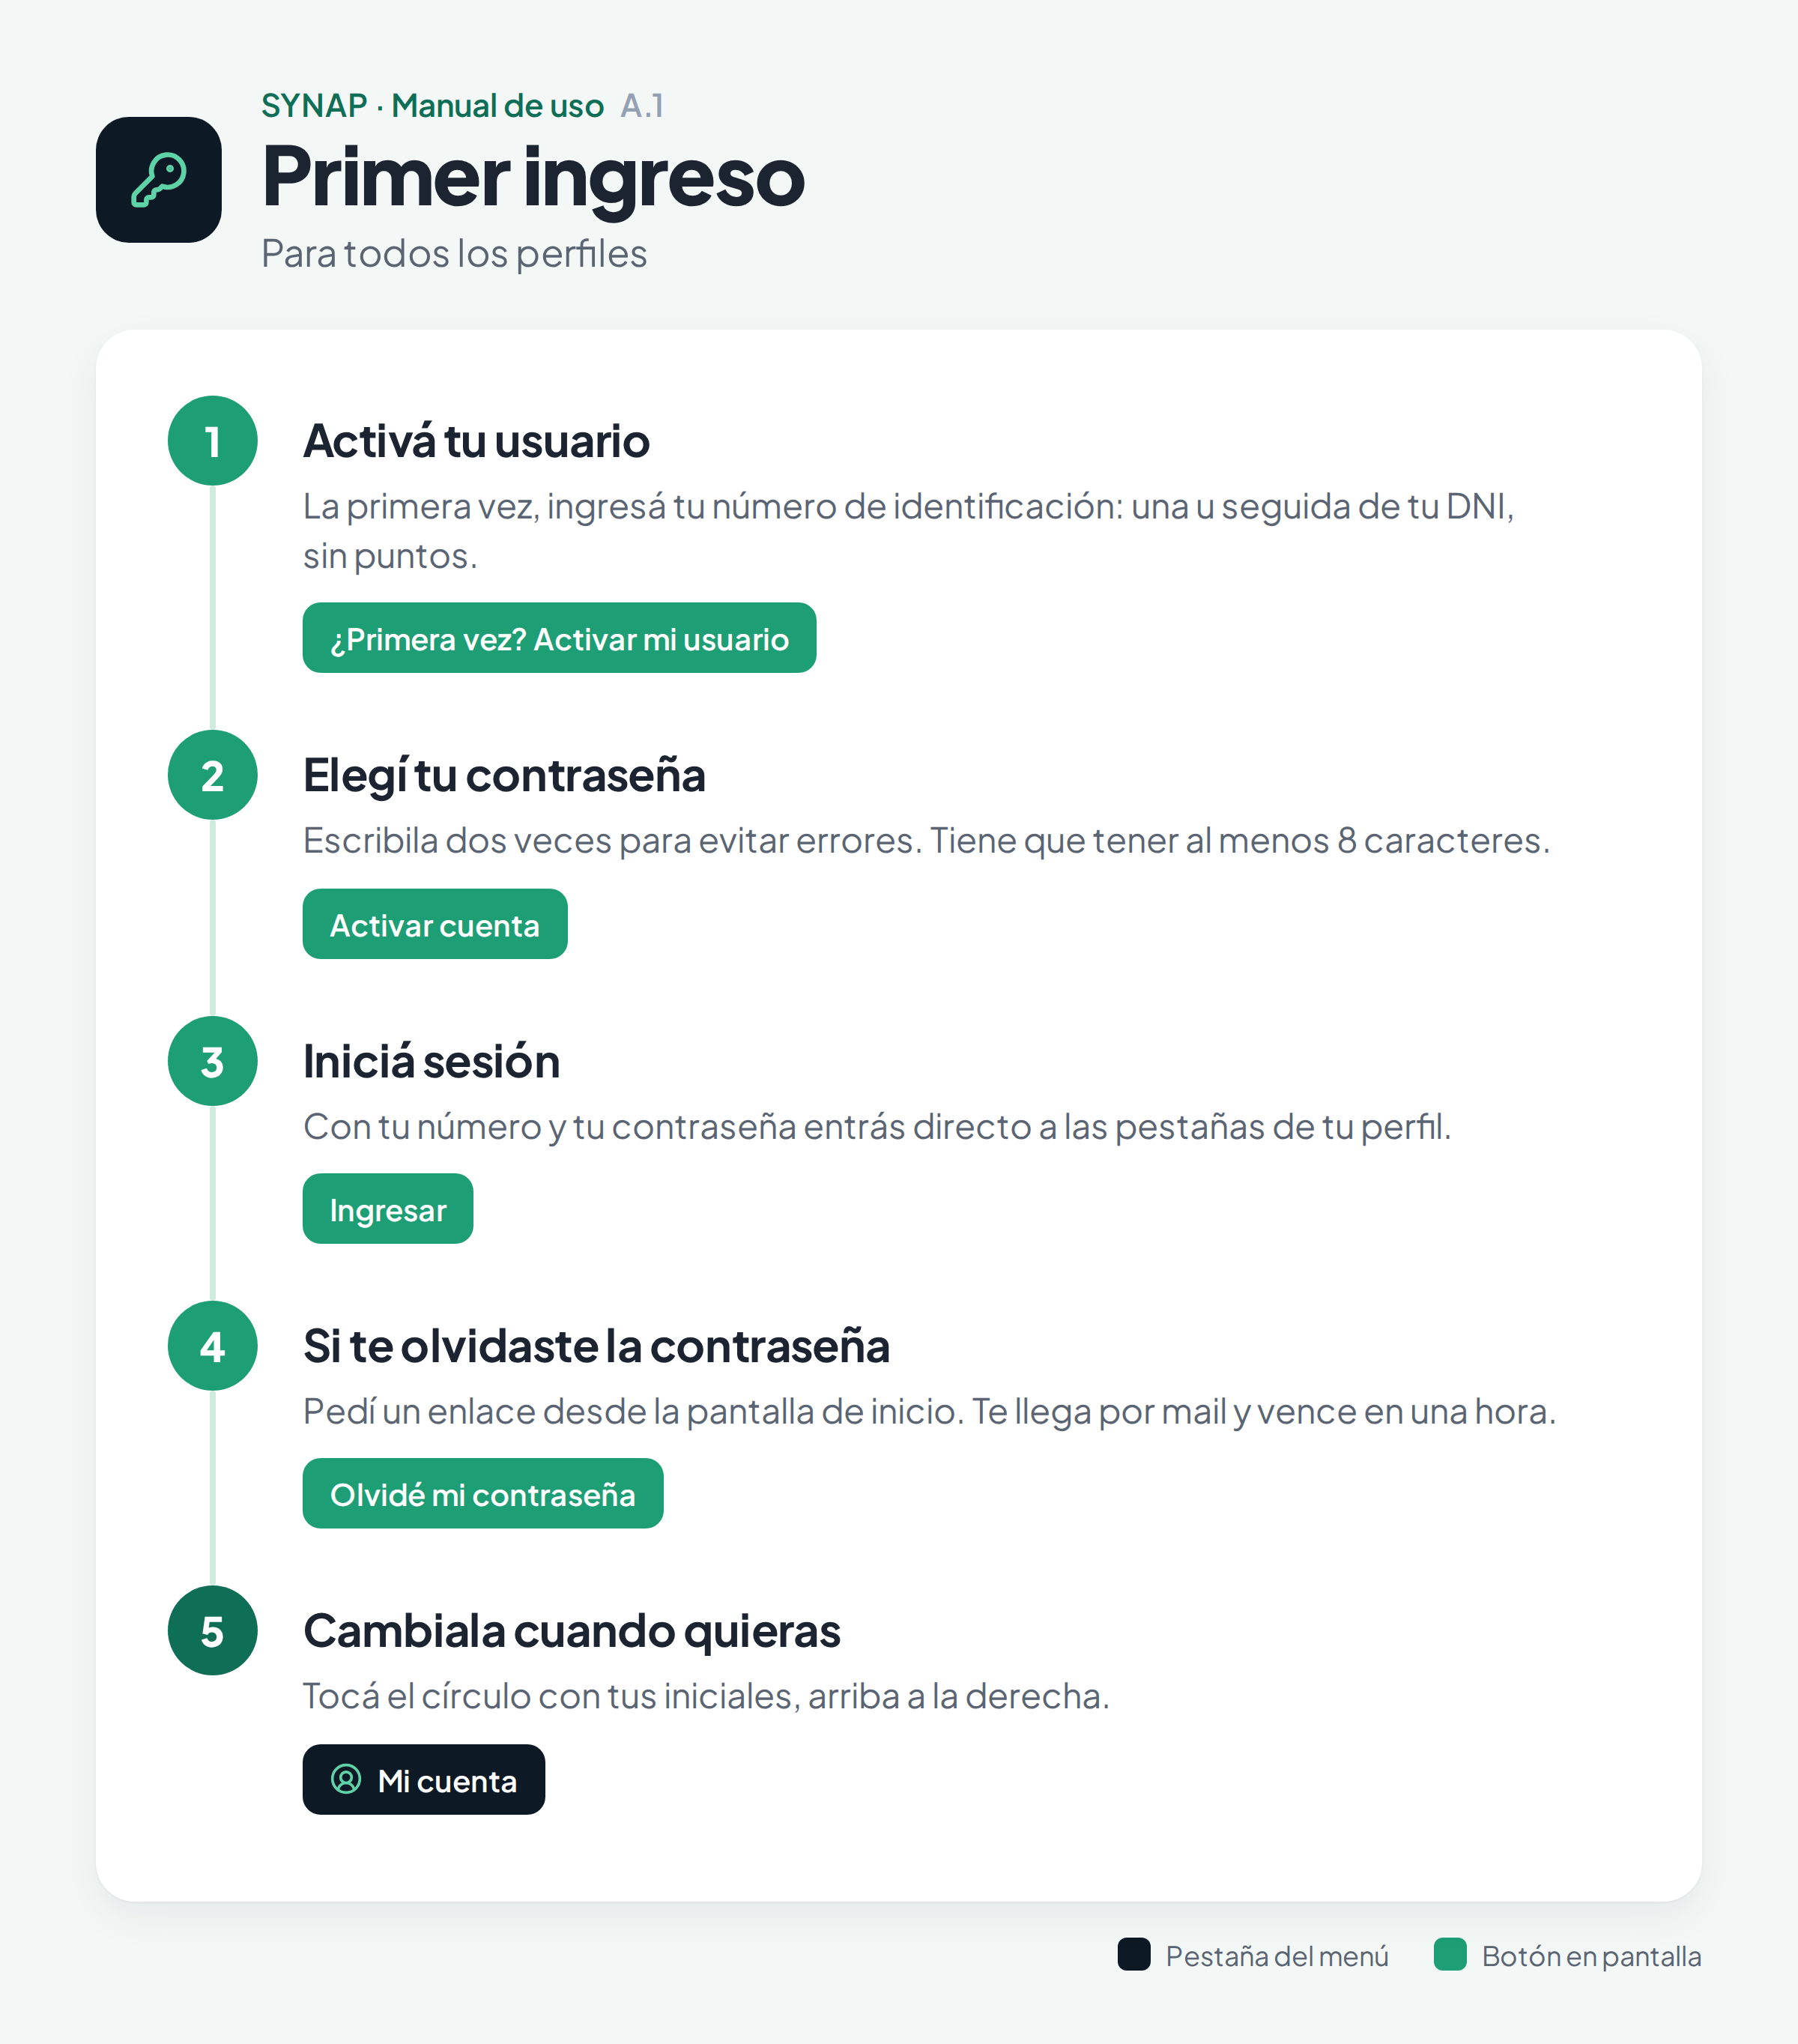
\includegraphics[height=\altomanual]{fotos/Manual_A1_primer_ingreso.png}
        \caption{Guía de primer ingreso al sistema, para todos los perfiles.}
        \label{fig:manual-a1}
    \end{minipage}
    \hfill
    \begin{minipage}[t]{0.47\linewidth}
        \centering
        
\includegraphics[height=\altomanual]{fotos/Manual_A3_tecnico.png}
        \caption{Guía de uso para el técnico: resolver órdenes y hacer los preventivos.}
        \label{fig:manual-a3}
    \end{minipage}
\end{figure}

\begin{figure}[H]
    \centering
    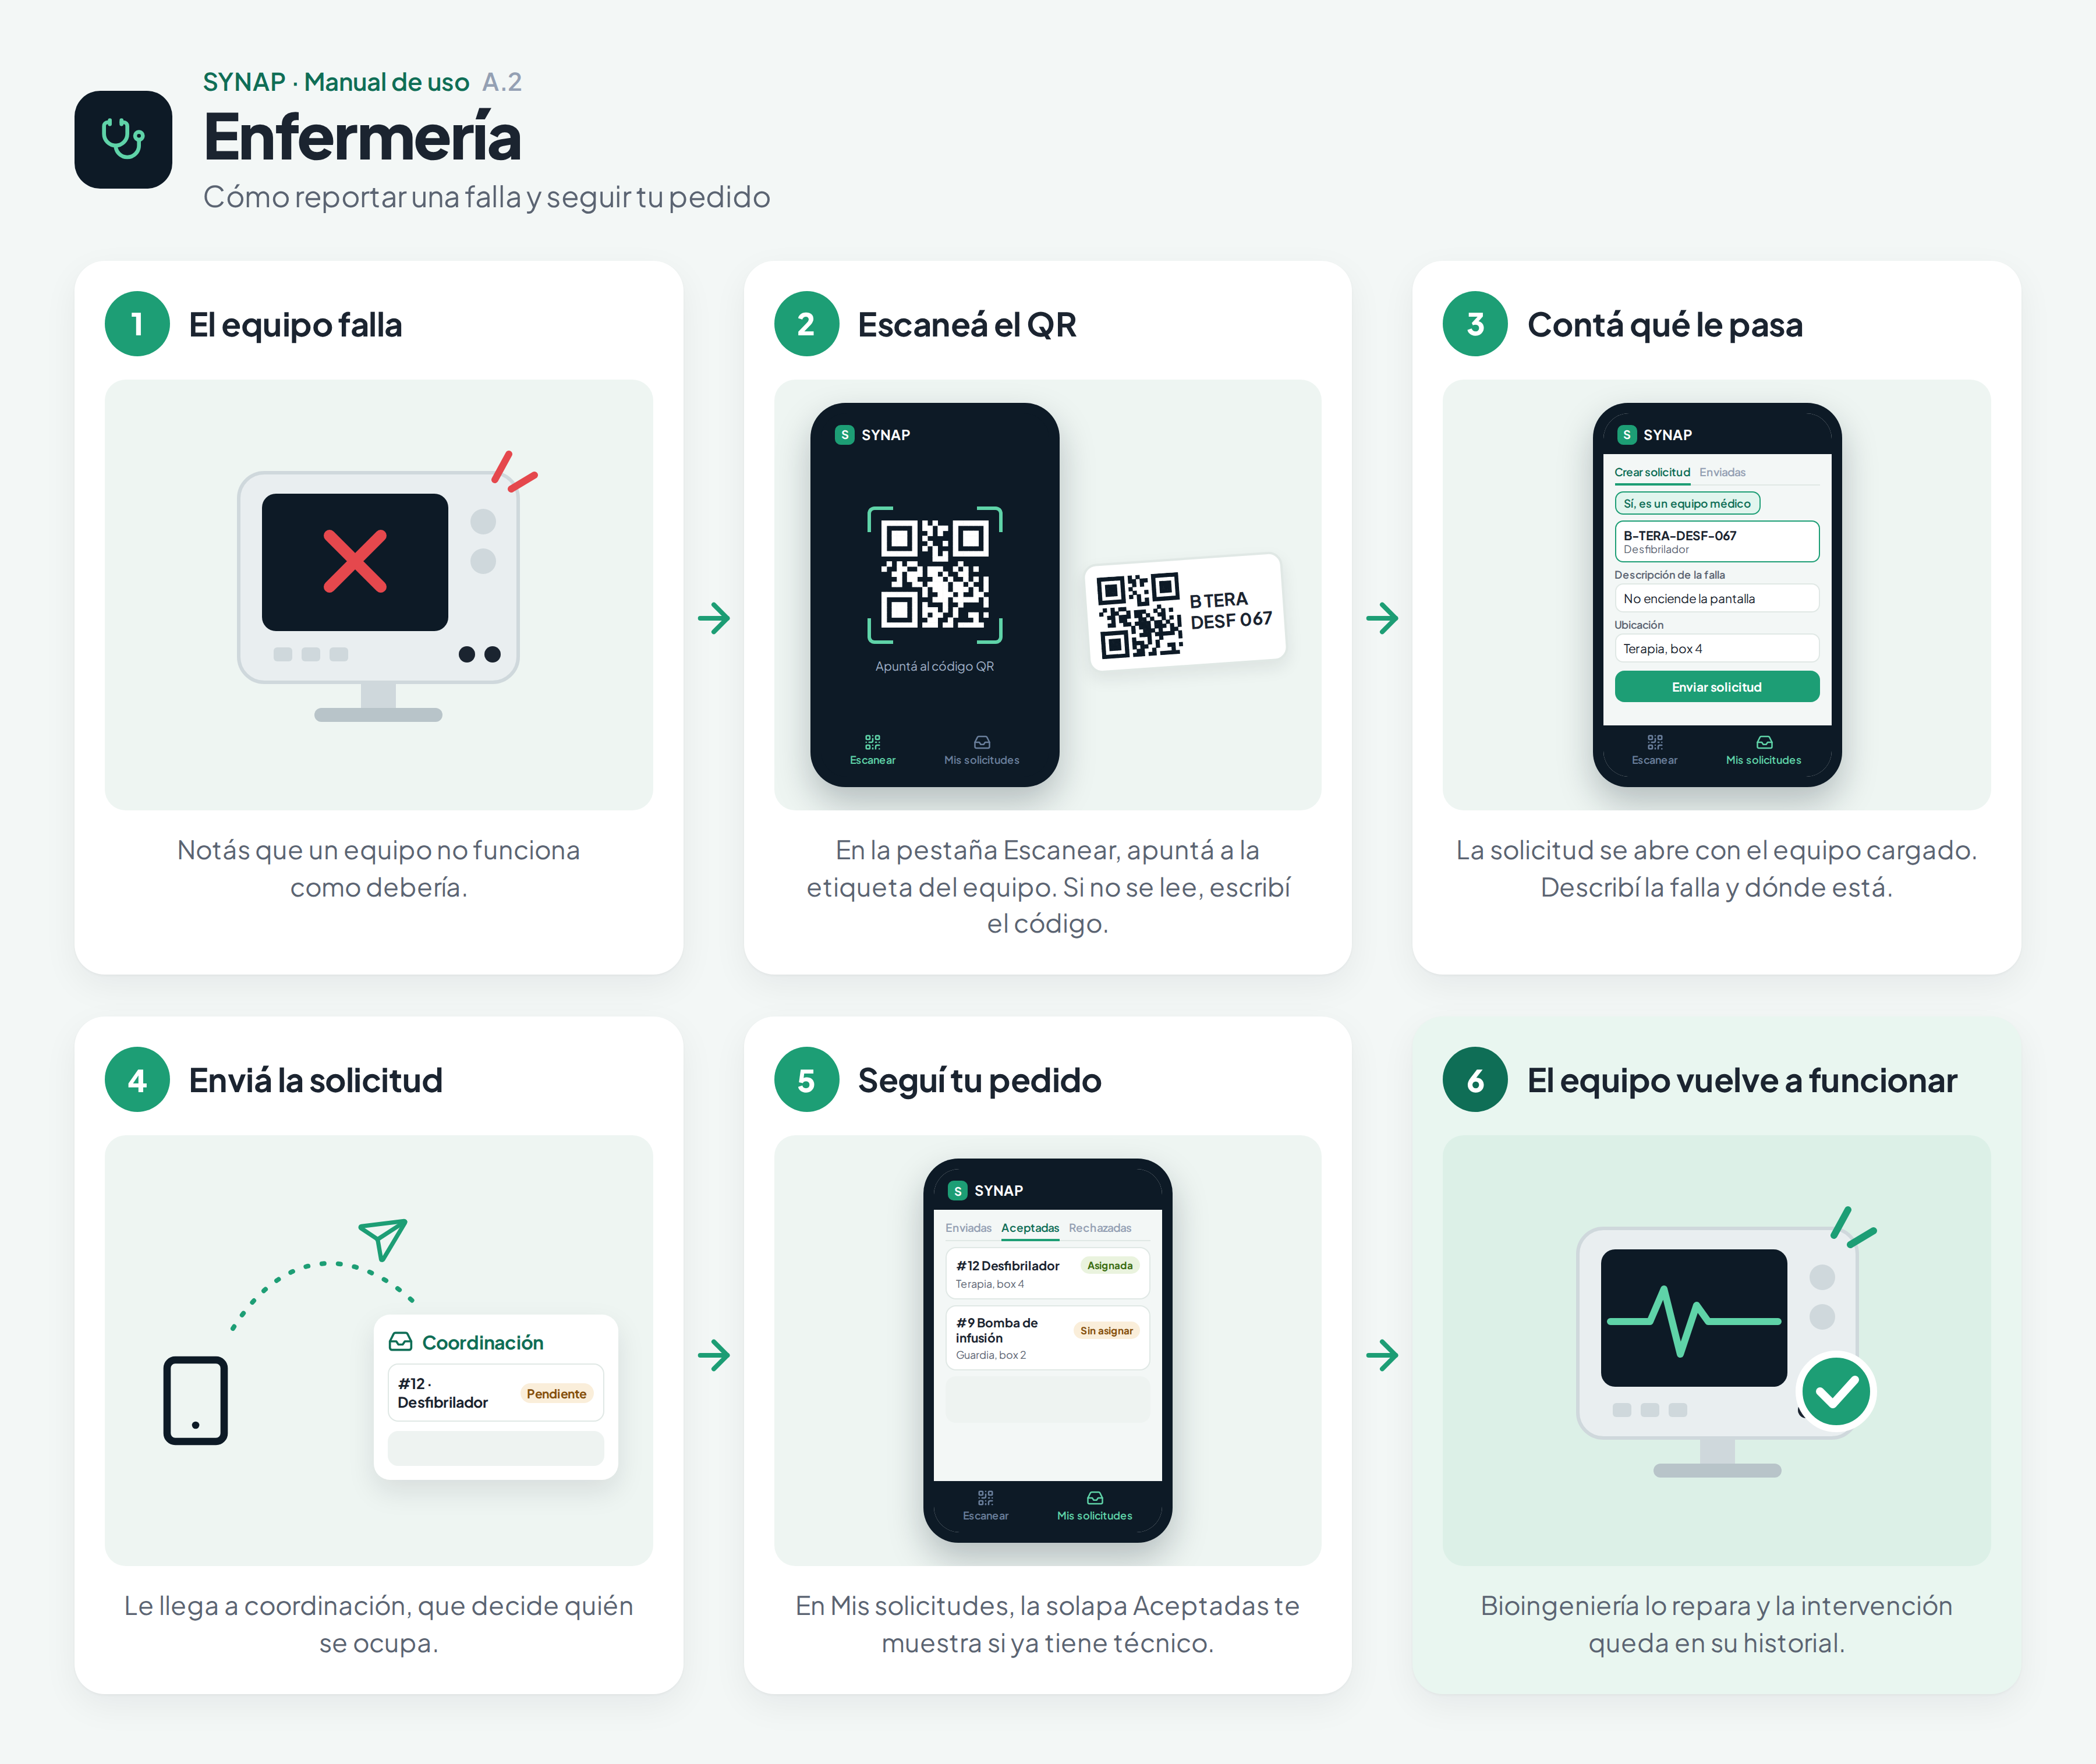
\includegraphics[width=0.65\linewidth,height=0.40\textheight,keepaspectratio]{fotos/Manual_A2_enfermeria_ilustrado.png}
    \caption{Guía de uso para enfermería: cómo reportar una falla y seguir el pedido.}
    \label{fig:manual-a2}
\end{figure}

\begin{figure}[H]
    \centering
    \setlength{\altomanual}{0.52\linewidth}
    \begin{minipage}[t]{0.43\linewidth}
        \centering
        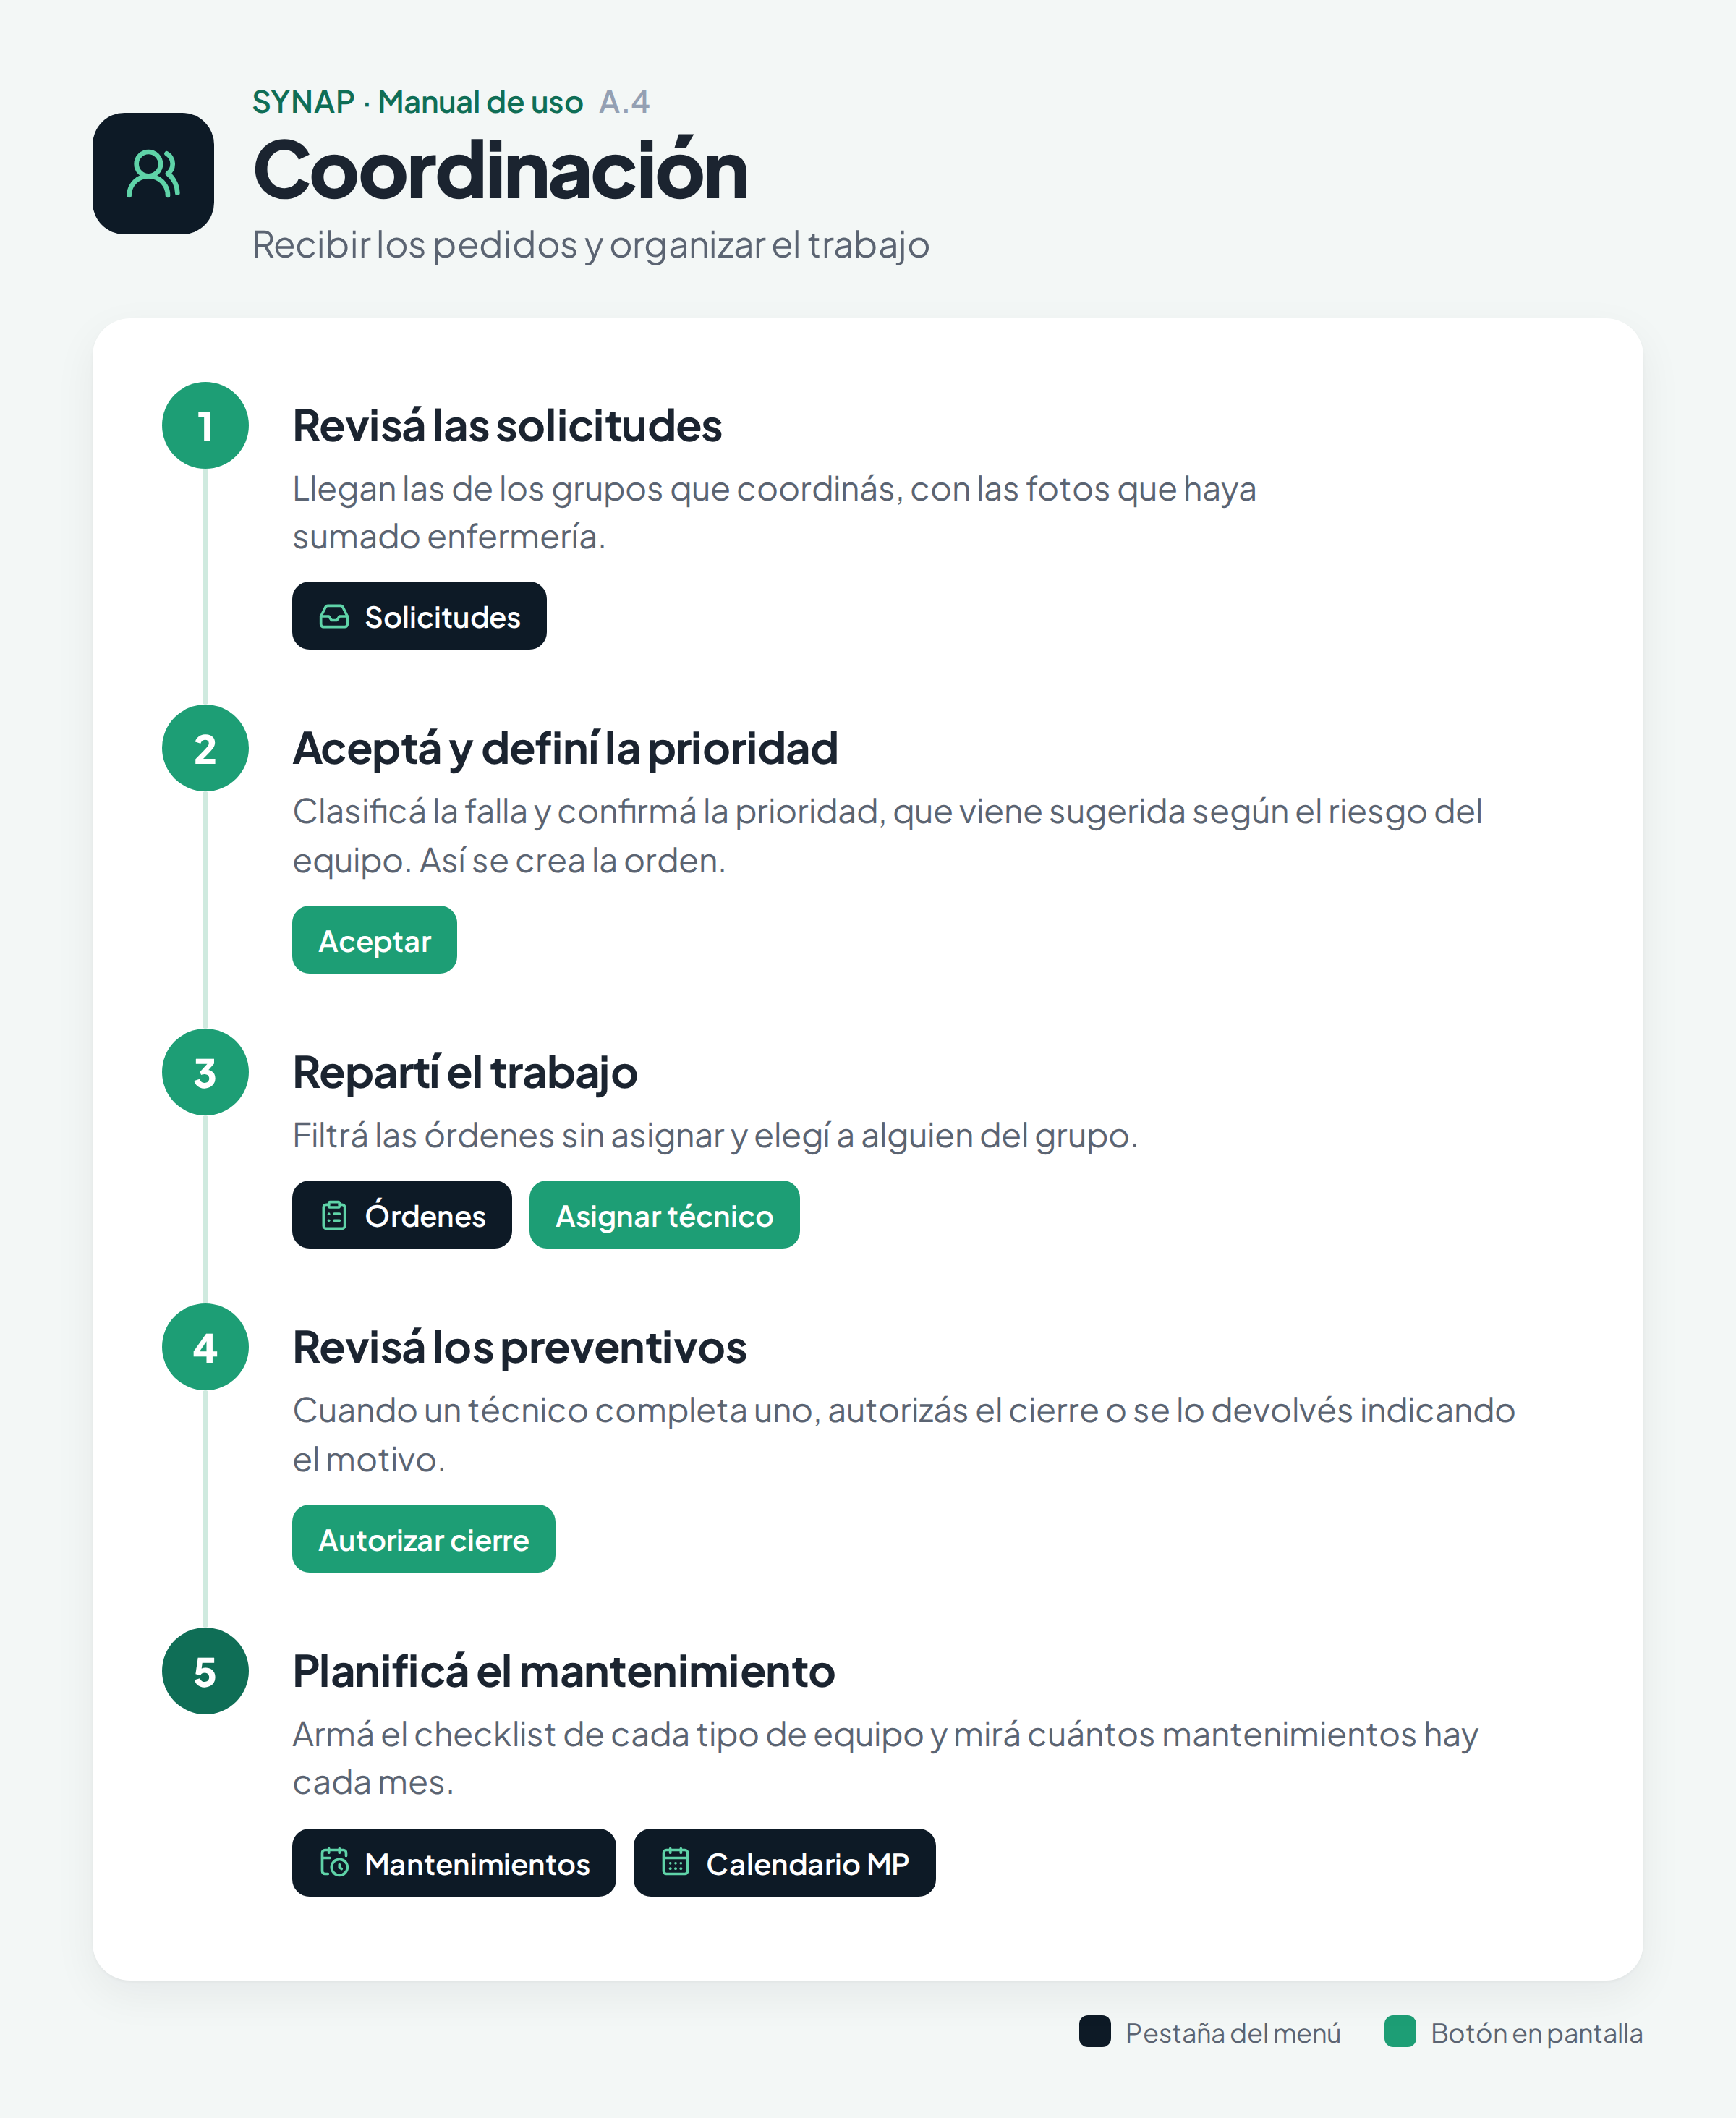
\includegraphics[height=\altomanual]{fotos/Manual_A4_coordinacion.png}
        \caption{Guía de uso para coordinación: recibir los pedidos y organizar el trabajo.}
        \label{fig:manual-a4}
    \end{minipage}
    \hfill
    \begin{minipage}[t]{0.53\linewidth}
        \centering
        
\includegraphics[height=\altomanual]{fotos/Manual_A5_jefatura.png}
        \caption{Guía de uso para jefatura: seguir el estado del servicio.}
        \label{fig:manual-a5}
    \end{minipage}
\end{figure}

\label{LastPage}

\end{document}